\documentclass{article}
\usepackage{iclr2027_conference,times}
\input{math_commands.tex}

\usepackage[utf8]{inputenc}
\usepackage[T1]{fontenc}
\usepackage{hyperref}
\usepackage{url}
\usepackage{booktabs}
\usepackage{amsfonts}
\usepackage{nicefrac}
\usepackage{microtype}
\usepackage{xcolor}
\usepackage{tabularx}
\usepackage{times}
\usepackage{soul}
\usepackage[normalem]{ulem}  % \uline for the sense-example table (Sec. 4.4)
\usepackage{caption}
\usepackage{graphicx}
\usepackage{subcaption}
\usepackage{amsmath}
\usepackage{amsthm}
\usepackage{amssymb}
\usepackage{algorithm}
\usepackage{algorithmicx}
\usepackage[noend]{algpseudocode}
\usepackage{multicol}
\usepackage{wrapfig}
\usepackage{multirow}
\usepackage{comment}
\usepackage{enumitem}
\usepackage{fancyvrb}
\usepackage{fvextra}
\usepackage{tikz}
\usetikzlibrary{positioning,shapes.geometric,shapes.misc,arrows.meta,fit,backgrounds}

\newtheorem{definition}{Definition}
\newtheorem{theorem}{Theorem}
\newtheorem{lemma}{Lemma}
\newtheorem{proposition}{Proposition}
\newtheorem{example}{Example}
\newtheorem{remark}{Remark}

\newcommand{\pr}[1]{\mathbb{P}\!\left( #1 \right)}
\newcommand{\coupling}[1]{\textsc{#1}}
\newcommand{\sense}[1]{\textsf{#1}}
\newcommand{\LCS}{\mathrm{LCS}}
\newcommand{\readout}[1]{\ensuremath{\mathrm{#1}}}
\newcommand{\mm}{\readout{mm}}
\newcommand{\cons}{\readout{cn}}
\newcommand{\rei}{\readout{re}}
\newcommand{\lp}{\readout{lp}}
\newcommand{\ent}{\coupling{entailment}}
\newcommand{\con}{\coupling{contradiction}}
\newcommand{\eqv}{\coupling{equivalence}}
\newcommand{\exc}{\coupling{exclusive}}
\newcommand{\cnc}{\coupling{co\_necessity}}

% Inline marker tying a span of response text to the claim it asserts, used in the
% verbalized responses of Sec. sec-example-pair.
\newcommand{\claimref}[1]{\mbox{\textcolor{blue!55!black}{\scriptsize[$a_{#1}$]}}}

% Verbatim style for the prompt appendix.
\DefineVerbatimEnvironment{promptverb}{Verbatim}%
  {fontsize=\scriptsize,frame=single,framesep=3pt,numbers=left,numbersep=3pt,
   breaklines=true,breakanywhere=true,commandchars=\\\{\}}
\newcommand{\promptfile}[1]{%
  \VerbatimInput[fontsize=\scriptsize,frame=single,framesep=3pt,numbers=left,
                 numbersep=3pt,breaklines=true,breakanywhere=true]{#1}}

% ---------------------------------------------------------------------------
% Shared tikz styles for the coherence figures (figures/graph-coherence-pair.tex,
% figures/mrf-coherence-pair.tex). Hoisted here so the panels of a two-panel
% figure cannot drift apart. Line width encodes the relation weight p via
% the relw=p style (see below); node fill encodes ground truth.
% ---------------------------------------------------------------------------
\tikzset{
  % --- claim variables -------------------------------------------------------
  atom/.style={circle,draw,fill=blue!5,inner sep=0.5pt,minimum size=6.2mm,
               font=\scriptsize},
  atomtrue/.style={atom,fill=blue!5,draw=blue!55!black},   % ground-truth TRUE
  atomfalse/.style={atom,fill=red!8,draw=red!60!black},    % ground-truth FALSE
  conf/.style={circle,draw,fill=red!8,draw=red!60!black,inner sep=0.5pt,
               minimum size=6.2mm,font=\scriptsize},
  hold/.style={circle,draw,fill=green!10,draw=green!45!black,inner sep=0.5pt,
               minimum size=6.2mm,font=\scriptsize},
  % --- couplings -------------------------------------------------------------
  ent/.style={-{Stealth[length=1.7mm]},blue!70!black},
  equ/.style={-{Stealth[length=1.7mm]},teal!70!black},
  con/.style={-{Stealth[length=1.7mm]},red!75!black,dashed},
  xcl/.style={{Stealth[length=1.7mm]}-{Stealth[length=1.7mm]},red!75!black,dashed},
  % --- MRF factor nodes ------------------------------------------------------
  factor/.style={rectangle,draw=black!75,fill=black!70,minimum size=1.9mm,
                 inner sep=0pt},
  unary/.style={factor,fill=black!35},
  flink/.style={black!55,line width=0.5pt},
  prlab/.style={font=\tiny,inner sep=1pt,text=black!70},
  wlab/.style={midway,font=\tiny,inner sep=1pt},
  % Relation weight p -> line width (lw ~ 0.6 + p pt), the AeroParts figure's
  % convention. A tikz STYLE rather than a macro, so pgfkeys sees the key=value
  % split before expansion; \dimexpr avoids needing \fpeval (absent in older TeX).
  relw/.style={line width=\the\dimexpr 0.6pt + #1pt\relax},
}

\algrenewcommand\algorithmicindent{0.6em}

%\iclrfinalcopy


\title{Beyond Individual Claims: Probabilistic Logical Coherence
       for Long-Form LLM Evaluation}

\author{Anonymous authors\\Paper under double-blind review}

% Float placement: the three result tables are wide but short; the defaults leave
% half-empty pages around them, so allow more float area per page.
\renewcommand{\topfraction}{0.95}
\renewcommand{\bottomfraction}{0.85}
\renewcommand{\textfraction}{0.05}
\renewcommand{\floatpagefraction}{0.90}
\setcounter{topnumber}{3}
\setcounter{bottomnumber}{2}
\setcounter{totalnumber}{4}

\begin{document}
\maketitle

\begin{abstract}
Long-form factuality assessment decomposes a response into atomic claims and verifies each against
retrieved evidence. The paradigm is effective and now standard, but it embeds an assumption --- that the
truth of each claim can be settled in isolation --- which discards the structure that makes prose an
argument. A response can therefore pass per-claim verification while contradicting itself, and two
responses built from \emph{identical} claims can differ in coherence through the order in which they
assert them. We formalize \emph{logical coherence} as a property of the joint distribution over claim
truth values induced by a Markov random field whose pairwise factors are the relations the response
itself draws. The relation vocabulary is a two-level taxonomy: twelve interpretable discourse senses,
grounded in PDTB~3.0 and RST, compile through a deterministic map onto five inferential couplings, each
fixing a factor table by naming the joint assignment it penalizes. We characterize the tables coherence
requires by a row-stochasticity property and show that those used for claim--evidence factuality are
wrong here, collapsing the measure's dynamic range; claim priors come from an existing factuality
pipeline, making coherence and factuality two stages over one decomposition. On a corpus of response
families whose coherence ordering is fixed by construction, the measure recovers $82.7\%$ of declared
orderings from gold relation graphs and $34.7$--$37.1\%$ from graphs mined out of the response text ---
and since the two conditions differ only in the relation graph, that gap localizes the open problem in
relation extraction rather than in the probabilistic model. Against five families of evidence-free
baselines it is the only measure that both orders responses correctly ($37/50$ against the best
baseline's $30/50$) and stays exactly invariant under meaning-preserving edits ($20/20$), the latter
\emph{by construction}: reordering sentences leaves the Markov network identical, a guarantee no surface
statistic can offer and one that an LLM judge violates while swinging $42$ points between judge models on
identical prose. The score also decomposes into per-claim marginals, so an incoherence is located rather
than merely detected.
\end{abstract}

%% ================================================================
\section{Introduction}
\label{sec-intro}
%% ================================================================

The dominant paradigm for assessing the factuality of long-form generation is decompose-then-verify:
split a response into atomic claims, check each against retrieved evidence, and aggregate the verdicts
\citep{factscore,safe,veriscore}. It is effective, it is now standard, and it embeds an assumption.
Treating each claim as independently checkable discards precisely the structure that distinguishes an
\emph{argument} from a \emph{list}.

Two failure modes make this concrete. A report may assert both that no passengers were harmed and that a wire
service reported three deaths; per-claim verification reports one claim true and one false, but not the more
basic defect --- that the response contradicts \emph{itself}. Separately, the inferential links a response
draws may fail even when their endpoints are individually true: a chain of accurate statements joined by a
spurious ``therefore'' is not a sound argument, and every atom in it verifies. \citet{lorefact} quantify how
often this matters: on logic-related samples, SAFE, VeriScore and FactCheck-GPT omit the logical dimension on
$60\%$, $78\%$ and $48\%$ of cases respectively. The two axes are orthogonal --- a response can be a bag of
true facts that is incoherent, or internally impeccable while entirely false --- and our sharpest fixture is a
pair of summaries of one appellate judgment built from the \emph{same} eighteen claims, one a permutation of
the other, differing only in whether self-serving assertions precede or follow the findings that qualify them:
every per-atom check returns an identical verdict, yet our measure separates them ($0.95$ against $0.90$).

% ---------------------------------------------------------------------------
% MOTIVATING FIGURE (Sec. sec-intro). Self-contained view of the five-claim
% Voyager 1 pair that Sec. sec-example later works formally and App. F.1 gives
% in full. Four bands, top to bottom:
%   (a) the two responses, abridged to their claim- and relation-bearing spans;
%   (b) the relation graphs those spans induce (transcribed from
%       figures/graph-coherence-pair.tex, so the two figures cannot diverge);
%   (c) the per-claim posterior marginals, with each claim's prior ticked;
%   (d) the scores and the gap.
% Every number is produced by scripts/lcs_worked_pair.py from
% data/lcs/example-7-coherence-pair.json -- exact, 2^5 = 32-world enumeration,
% computed twice by independent paths and asserted equal. Do not edit a value
% here without rerunning that script.
% Node, edge and relw=p styles live in preamble.tex, shared with the Sec. 3.7
% and App. F figures, so no panel can drift from another. The two graph panels
% are drawn at ONE fixed scale (\mtvscale) rather than each in its own
% \resizebox, so a difference in bounding box cannot make one look larger.
% ---------------------------------------------------------------------------
\begin{figure}[p]
\centering
\footnotesize
\setlength{\tabcolsep}{0pt}
% one shared scale for both relation graphs
\newcommand{\mtvx}{13.2mm}
\newcommand{\mtvy}{11.6mm}

%% ===== band (0): the query both responses answer =========================
% Grey and unadorned: it belongs to neither response, and the point of showing
% it is that BOTH answer it. Its two parts are why a good answer must both
% assert a3 and dispatch the a5 confusion.
\colorbox{black!5}{\parbox{\dimexpr\textwidth-2\fboxsep\relax}{\centering
  \scriptsize \textbf{Query}\ \ \emph{Where is Voyager~1 now, and has it left
  the Solar System?}\strut}}

\smallskip
%% ===== band (a): the two responses ======================================
% Both boxes are set to ONE height (\mtvbox), so the pair aligns top and bottom
% however the two texts happen to break. Raise it if either box overflows.
\newcommand{\mtvbox}{33.5mm}
\begin{tabularx}{\textwidth}{@{}X@{\hspace{7pt}}X@{}}
\begin{minipage}[t]{\linewidth}
  \colorbox{blue!4}{\parbox[t][\mtvbox][t]{\dimexpr\linewidth-2\fboxsep\relax}{%
  \textbf{\textcolor{blue!55!black}{Response A}} \; \emph{coherent}\\[2pt]
  \scriptsize
  Voyager~1 crossed the heliopause in August 2012,\,\claimref{1} and in the days
  that followed its instruments measured a sharp rise in plasma
  density\,\claimref{2} --- \emph{the measurement that established the boundary
  had been passed.} Voyager~1 is therefore in interstellar space.\,\claimref{3}
  Two persistent misconceptions are worth clearing up. The first is that the
  plasma wave instrument had failed permanently before the
  crossing;\,\claimref{4} \emph{it cannot have, since it is precisely that
  instrument which returned the density profile the conclusion rests on.} The
  second is that Voyager~1 has left the Solar System
  altogether.\,\claimref{5} \emph{Being in interstellar space is not the same
  thing: the Sun's gravitational reach extends through the Oort cloud.}\strut}}
\end{minipage}
&
\begin{minipage}[t]{\linewidth}
  \colorbox{red!4}{\parbox[t][\mtvbox][t]{\dimexpr\linewidth-2\fboxsep\relax}{%
  \textbf{\textcolor{red!60!black}{Response B}} \; \emph{incoherent}\\[2pt]
  \scriptsize
  Voyager~1 crossed the heliopause in August 2012,\,\claimref{1} and after the
  crossing its instruments measured a sharp rise in plasma
  density.\,\claimref{2} \emph{That said, the probe cannot really be counted as
  being in interstellar space.}\,\claimref{3} The plasma wave instrument had
  \textbf{in fact} failed permanently before the crossing,\,\claimref{4}
  \emph{and it is precisely that failure which tells us the probe reached
  interstellar space.} \emph{The instrument failure also means} Voyager~1 has
  left the Solar System entirely.\,\claimref{5} \emph{Of course, the crossing
  rules out any such failure, and the density measurement is inconsistent with
  the probe having left the Solar System.}\strut}}
\end{minipage}
\end{tabularx}

\smallskip
{\scriptsize
  \textbf{The same five claims} $a_1,\dots,a_5$ (\claimref{i} marks each first
  mention) $\Rightarrow$ \textbf{identical per-claim factuality verdicts.}
  Only the italicized \emph{relation-bearing} spans differ.}

\medskip
%% ===== band (b): the relation graphs, at one shared scale ===============
\begin{tabularx}{\textwidth}{@{}X@{\hspace{7pt}}X@{}}
\begin{minipage}[b]{\linewidth}\centering
\begin{tikzpicture}[x=\mtvx, y=\mtvy]
  \node[atomtrue]  (a1) at (0,0)        {$a_1$};
  \node[atomtrue]  (a2) at (1.15,0)     {$a_2$};
  \node[atomtrue]  (a3) at (2.3,0)      {$a_3$};
  \node[atomfalse] (a4) at (1.7,-1.55)  {$a_4$};
  \node[atomfalse] (a5) at (2.9,-1.55)  {$a_5$};

  \node[prlab,above=0.4mm of a1] {$\pi{=}.9$};
  \node[prlab,above=0.4mm of a2] {$\pi{=}.9$};
  \node[prlab,above=0.4mm of a3] {$\pi{=}.9$};
  \node[prlab,below=0.4mm of a4] {$\pi{=}.1$};
  \node[prlab,below=0.4mm of a5] {$\pi{=}.1$};

  \draw[ent,relw=0.90] (a1) -- (a2) node[wlab,above]{$.90$};
  \draw[ent,relw=0.85] (a2) -- (a3) node[wlab,above]{$.85$};
  \draw[con,relw=0.90] (a3) -- (a4) node[wlab,left,pos=0.5]{$.90$};
  \draw[con,relw=0.85] (a3) -- (a5) node[wlab,right,pos=0.5]{$.85$};

  \node[font=\tiny,align=center,text=black!65,anchor=north] at (0.45,-0.90)
       {both conflicts point\\\emph{outward}, at the\\two false claims};
  % invisible strut matching panel B's annotation depth, so the two panels
  % share a baseline instead of one riding higher than the other.
  \path (0.45,-2.62) -- (0.45,0.98);
\end{tikzpicture}\\[3pt]
{\scriptsize \textbf{A:} a support chain over the true claims;
 each false claim \emph{attributed, then refused} from $a_3$.}
\end{minipage}
&
\begin{minipage}[b]{\linewidth}\centering
\begin{tikzpicture}[x=\mtvx, y=\mtvy]
  % Six edges over five nodes, so B needs more room than A: the two false
  % claims sit a full row lower and the row is wider, which keeps the
  % a4 -> a3 edge and the a2 -> a5 curve from crossing on top of each other.
  \node[atomtrue]  (a1) at (0,0)        {$a_1$};
  \node[atomtrue]  (a2) at (1.15,0)     {$a_2$};
  \node[atomtrue]  (a3) at (2.3,0)      {$a_3$};
  \node[atomfalse] (a4) at (0.55,-1.55) {$a_4$};
  \node[atomfalse] (a5) at (1.75,-1.55) {$a_5$};

  % Priors sit clear of the two orange change annotations.
  \node[prlab,above=0.4mm of a1] {$\pi{=}.9$};
  \node[prlab,above=0.4mm of a3] {$\pi{=}.9$};
  \node[prlab,above=0.4mm of a2] {$\pi{=}.9$};
  \node[prlab,left=0.5mm of a4]  {$\pi{=}.1$};
  \node[prlab,right=0.5mm of a5] {$\pi{=}.1$};

  \draw[ent,relw=0.90] (a1) -- (a2) node[wlab,above]{$.90$};
  \draw[con,relw=0.90] (a2) -- (a3) node[wlab,above]{$.90$};
  % the reversed edge: the false a4 now feeds the true a3
  \draw[ent,relw=0.88] (a4) -- (a3)
        node[wlab,above left=-0.4mm and -1.0mm,pos=0.30]{$.88$};
  \draw[con,relw=0.90] (a1) -- (a4) node[wlab,left,pos=0.55]{$.90$};
  \draw[ent,relw=0.85] (a4) -- (a5) node[wlab,below]{$.85$};
  % a2 -> a5 swings out to the right of a5 so it never lands on a4 -> a3
  \draw[con,relw=0.88] (a2) to[out=-8,in=25]
        node[wlab,right,pos=0.55,inner sep=1pt]{$.88$} (a5);

  % --- the two changes that carry the whole difference ---------------------
  % The two annotations are numbered and placed in the free space to the
  % RIGHT of the graph and BELOW it, so neither overlays a prior label, an
  % edge, or a weight. Each carries a dotted leader to what it marks.
  % (1) marks the a2--a3 edge, whose coupling flipped.
  \node[chgnum] (n1) at (2.98,-0.46) {1};
  \draw[chglead] (n1) -- (1.90,-0.06);
  % (2) rings a4, whose role reversed. The ring is drawn BEHIND the node so it
  % cannot cover the label; the number sits outside it.
  \begin{scope}[on background layer]
    \node[chg,circle,minimum size=9.4mm,inner sep=0pt] at (0.55,-1.55) {};
  \end{scope}
  \node[chgnum] (n2) at (-0.42,-1.05) {2};
  \draw[chglead] (n2) -- (0.22,-1.35);
  \node[chglab,anchor=north west,align=left] at (2.55,-0.75)
       {\textbf{1} support $\to$ \con{}:\\B denies its own\\conclusion $a_3$};
  \node[chglab,anchor=north,align=center] at (0.9,-2.20)
       {\textbf{2} the arrow \emph{reverses}: the false $a_4$\\is now a premise
        \emph{for} the true $a_3$};
\end{tikzpicture}\\[3pt]
{\scriptsize \textbf{B:} the same five claims, \emph{rearranged}. Half its
 conflicts point \emph{inward}, at what it asserts.}
\end{minipage}
\end{tabularx}

\medskip
%% ===== band (c): the per-claim posteriors ===============================
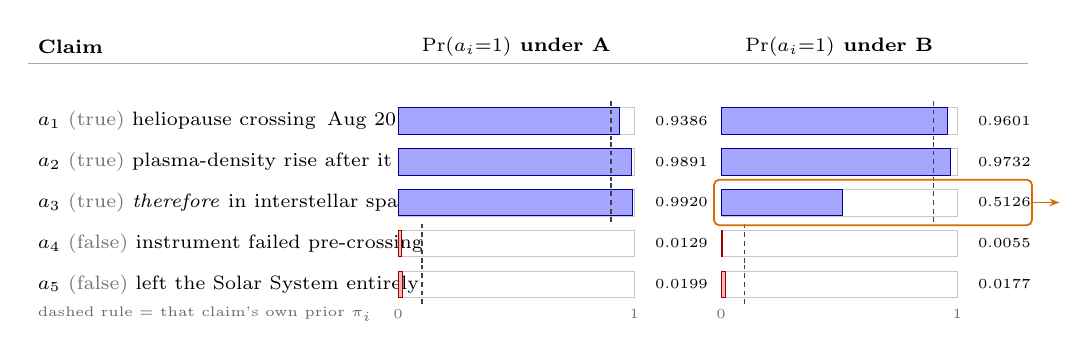
\begin{tikzpicture}[x=1mm, y=1mm]
  \def\bw{30}          % bar-track width
  \def\rh{5.2}         % row height
  \def\ca{47}          % left edge, track A
  \def\cb{88}          % left edge, track B

  \node[font=\bfseries\scriptsize,anchor=west] at (0,4.2)  {Claim};
  \node[font=\bfseries\scriptsize] at (\ca+0.5*\bw,4.2)    {$\Pr(a_i{=}1)$ under A};
  \node[font=\bfseries\scriptsize] at (\cb+0.5*\bw,4.2)    {$\Pr(a_i{=}1)$ under B};
  \draw[black!35,line width=0.3pt] (0,2.0) -- (127,2.0);

  % {i}{prior}{postA}{postB}{fill}{edge}{tag}{gloss} -- the colour is carried in
  % the list rather than branched on, so no \ifthenelse (not loaded) is needed.
  \foreach \i/\pri/\pa/\pb/\bc/\ec/\tag/\gloss in {%
      1/0.9/0.9386/0.9601/blue!35!white/blue!55!black/true/heliopause crossing\, Aug 2012,
      2/0.9/0.9891/0.9732/blue!35!white/blue!55!black/true/plasma-density rise after it,
      3/0.9/0.9920/0.5126/blue!35!white/blue!55!black/true/{\emph{therefore} in interstellar space},
      4/0.1/0.0129/0.0055/red!30!white/red!60!black/false/instrument failed pre-crossing,
      5/0.1/0.0199/0.0177/red!30!white/red!60!black/false/left the Solar System entirely}
  {
    \pgfmathsetmacro{\y}{-\i*\rh}
    \node[anchor=west,font=\scriptsize] at (0,\y)
         {$a_\i$ \textcolor{black!55}{(\tag)}\ \gloss};
    \foreach \x in {\ca,\cb}{
      \draw[black!22,line width=0.25pt] (\x,\y-1.7) rectangle (\x+\bw,\y+1.7);
    }
    \pgfmathsetmacro{\wa}{\pa*\bw}
    \pgfmathsetmacro{\wb}{\pb*\bw}
    \fill[\bc,draw=\ec,line width=0.3pt] (\ca,\y-1.7) rectangle (\ca+\wa,\y+1.7);
    \fill[\bc,draw=\ec,line width=0.3pt] (\cb,\y-1.7) rectangle (\cb+\wb,\y+1.7);
    % each claim's own prior, as a tick across the track
    \foreach \x in {\ca,\cb}{
      \pgfmathsetmacro{\tk}{\x+\pri*\bw}
      \draw[black!75,line width=0.6pt,dash pattern=on 0.6mm off 0.5mm]
            (\tk,\y-2.5) -- (\tk,\y+2.5);
    }
    \node[anchor=west,font=\tiny] at (\ca+\bw+1.4,\y) {\pa};
    \node[anchor=west,font=\tiny] at (\cb+\bw+1.4,\y) {\pb};
  }

  % the diagnostic callout: a3 under B
  \pgfmathsetmacro{\ythree}{-3*\rh}
  \draw[orange!85!black,line width=0.65pt,rounded corners=0.7mm]
        (\cb-0.9,\ythree-2.9) rectangle (\cb+\bw+9.5,\ythree+2.9);
  \draw[orange!85!black,line width=0.5pt,-{Stealth[length=1.3mm]}]
        (\cb+\bw+9.5,\ythree) -- (\cb+\bw+13,\ythree);

  \foreach \x in {\ca,\cb}{
    \node[font=\tiny,text=black!55] at (\x,-5*\rh-3.8)     {$0$};
    \node[font=\tiny,text=black!55] at (\x+\bw,-5*\rh-3.8) {$1$};
  }
  \node[font=\tiny,text=black!60,anchor=west] at (0,-5*\rh-3.8)
       {dashed rule $=$ that claim's own prior $\pi_i$};
\end{tikzpicture}

\smallskip
{\footnotesize\raggedright
\textcolor{orange!55!black}{\textbf{The diagnostic.}} $a_3$ is \textbf{true of
the world}, yet B drags it to a coin flip --- $0.992 \to 0.513$, far below its
own $0.9$ prior --- because its only support now arrives from $a_4$, a claim
the response itself denies. No aggregate score reveals this; a per-claim
marginal locates it.\par}

\medskip
%% ===== band (d): the scores =============================================
\begin{tabularx}{\textwidth}{@{}p{31mm}@{\hspace{8pt}}X@{}}
\toprule
\small\textbf{Coherence score}
& \small $\LCS_{\mm}$:\quad
  \textcolor{blue!55!black}{\textbf{$0.590$}}~(A)
  \ \ $\longrightarrow$\ \
  \textcolor{red!60!black}{\textbf{$0.494$}}~(B)
  \qquad $\boldsymbol{\Delta = -0.097}$ \\
\scriptsize\textcolor{black!60}{exact, by $2^5{=}32$-world enum.}
& \scriptsize $\LCS_{\cons}$: $0.963 \to 0.414$ \ \textbullet\
  $\log Z$: $-0.95 \to -3.78$ \ \textbullet\
  prior-only baseline $0.580$ (A \emph{above} it, B \emph{below}) \\
\midrule
\multicolumn{2}{@{}X@{}}{\scriptsize The priors enter \emph{only} through the
  unary factors, which are identical in the two responses. The entire
  $0.590\to0.494$ drop is produced by the pairwise relation factors --- that
  is, by \textbf{arrangement alone}.} \\
\bottomrule
\end{tabularx}

% scripts/make_motivating_png.sh defines \mtvnocaption to render the figure
% for standalone export, where the surrounding prose supplies the explanation.
% Undefined in the paper, so the caption below is typeset normally there.
\ifdefined\mtvnocaption\else
\caption{\textbf{Two responses, the same five claims, different coherence.}
  Five claims about Voyager~1 are fixed once and for all: $a_1,a_2,a_3$ true of
  the world (priors $\pi_i{=}0.9$, blue) and $a_4,a_5$ false ($\pi_i{=}0.1$,
  red). Both responses answer the \emph{same} query and assert \emph{all five}
  claims, so every per-claim factuality check returns the same verdict on both
  and no decompose-then-verify score can separate them. \textbf{A} attributes the two falsehoods and then refuses each
  on a stated ground; \textbf{B} asserts them and reasons \emph{from} them,
  offering the false $a_4$ as the reason the true $a_3$ holds while denying
  $a_3$ outright --- then denying $a_4$ and $a_5$ in its closing sentence.
  Middle: the relation graphs those spans induce (solid blue \ent{}, dashed red
  \con{}, line width growing with the mined weight $p$), drawn at one shared
  scale; the two numbered orange callouts \textbf{1} and \textbf{2} mark the
  only two changes, which carry the whole difference. Bottom: the posterior marginals of the coherence MRF, and the
  score. Mentioning a falsehood is not what costs B its score; asserting it and
  reasoning from it is. \S\ref{sec-example} works this pair formally and
  App.~\ref{app-examples} gives both responses in full.}
\label{fig:motivating}
\fi
\end{figure}


\paragraph{A motivating example.}
Figure~\ref{fig:motivating} shows the failure in the smallest instance we can enumerate exactly, and it is
worth reading in full because every later section is an answer to something visible in it. Five claims about
Voyager~1 are fixed once and for all: three true of the world and two false. \emph{Both} responses assert all
five, so the two are indistinguishable to any method that scores claims one at a time --- every retrieval,
every NLI check, every per-atom verdict is byte-identical across the pair, and a precision-style aggregate
returns $3/5$ for both. What differs is the argument the response builds out of them. Response~A names the two
falsehoods, attributes them, and refuses each on a stated ground; Response~B asserts them as fact, offers the
false $a_4$ (``the plasma wave instrument had failed'') as the \emph{reason} the true $a_3$ (``therefore in
interstellar space'') holds, and in the same breath denies $a_3$ outright --- then denies $a_4$ and $a_5$ in
its closing sentence. Read as prose, B is fluent; read as an argument, it is incoherent, and its incoherence is
not located in any one claim but in the wiring between them.

Two changes in the relation graph carry the entire difference (callouts \textbf{1} and \textbf{2} in the figure): the support
edge $a_2\!\to\!a_3$ becomes a \con{}, and the edge between $a_3$ and $a_4$ \emph{reverses} --- what A uses to
reject a falsehood, B uses to lean on one. Our measure scores A at $\LCS_{\mm}=0.590$ against B's $0.494$
(exact, by $2^5$ enumeration), and because the priors enter only through unary factors that are identical in
the two panels, the whole drop is attributable to arrangement alone. Mentioning a falsehood is not what costs B
its score; asserting it and reasoning from it is. The score also localizes the damage, which an aggregate
cannot: the \emph{true} claim $a_3$ finishes at $0.513$ under B against $0.992$ under A, dragged below its own
$0.9$ prior because its only support now arrives from a claim the response itself denies --- and a premise the
text refuses cannot transmit support. A claim true of the world is demoted to a coin flip by the argument built
around it. \S\ref{sec-example} works this pair formally once the model is in place, and
App.~\ref{app-examples} gives both responses verbatim alongside three further examples.

We therefore ask: how much of what a response asserts does its argument, taken as a whole, uphold? That is
answered by a \emph{marginal} in a graphical model whose variables are claim truth values and whose factors
are the asserted relations --- not by counting violated rules, which cannot propagate a conflict from its
endpoints to what they support, and which yields a measure a response maximizes by asserting no relations at
all (Prop.~\ref{prop-vacuous}).

Our contributions are as follows. (i) A \textbf{coherence MRF and a formal two-level relation taxonomy}
(\S\ref{sec-mrf}--\S\ref{sec-levels}): twelve discourse senses compile through a deterministic map onto five
inferential couplings, each defined by the joint assignment it penalizes, which fixes its factor table ---
separating the interpretable layer from the inferential one lets the annotation vocabulary be rich while the
model stays a closed three-parameter pairwise family. (ii) A \textbf{characterization of why factuality's
factor tables are wrong for coherence} (\S\ref{sec-potentials}): they charge a premise for being a premise, and
the alternative collapses the measure's dynamic range by more than half. (iii) A \textbf{selected readout and a
two-stage composition with factuality} (\S\ref{sec-score}, \S\ref{sec-twostage}): of four candidates evaluated
by exact inference against five criteria, only two are monotone in conflict resolution. (iv) \textbf{An evaluation
separating relation-extraction error from scoring error} (\S\ref{sec-experiments}), by holding the readouts
byte-identical and swapping only the relation graph: the measure satisfies $82.7\%$ of $202$ declared constraints
from gold graphs against $34.7$--$37.1\%$ from mined ones, localizing the open problem in extraction; and against
five families of evidence-free baselines it is the only one that both orders responses correctly ($37/50$ against
the best baseline's $30/50$) and is exactly invariant under meaning-preserving edits ($20/20$) --- the latter \emph{by
construction}, a guarantee no surface statistic can offer.

%% ================================================================
\section{Related Work}
\label{sec-related}
%% ================================================================

\paragraph{Atomic factuality.} FActScore \citep{factscore} introduced per-atom precision against a knowledge
source; SAFE \citep{safe} added search-augmented verification and an $F_1@K$ metric, VeriScore
\citep{veriscore} restricted attention to \emph{verifiable} claims, and FLEEK \citep{fleek} retrieves evidence
to detect and correct errors. All aggregate independent per-claim verdicts and are therefore blind to
inter-claim structure by construction. FactReasoner \citep{factreasoner} replaced verdict counting with
probabilistic inference over a factor graph of claim and evidence variables with pairwise factors from NLI
relations; it is the closest antecedent --- we reuse its decomposition, relation extractor and inference
stack, and take its marginals as our priors (\S\ref{sec-twostage}) --- but its factors run between a claim and
the \emph{evidence} retrieved for it, so its graph has no claim--claim edges and its marginals cannot express
internal consistency. \citet{lorefact} states the gap directly, classifying inter-atom dependencies as a
labelling task over claim pairs; our departure is to treat them as \emph{factors in a joint distribution},
which lets a local conflict propagate to distant claims and makes the score a functional of the whole graph
rather than a per-edge average.



\paragraph{Discourse coherence.} Entity-grid models \citep{barzilay} and their neural successors \citep{li}
score coherence from entity-mention distributions, evaluated against \emph{synthetic perturbations} --- a
methodology we extend in \S\ref{sec-protocol} by making the perturbation an operator on a declared relation
graph rather than on raw text, so its intended effect is known per item. DiscoScore \citep{discoscore} uses
BERT-based discourse representations. What these share is that coherence is read off surface statistics or
learned representations: none exposes an inspectable relation graph, and none yields per-claim attributions.
Our inventory takes its senses from PDTB~3.0 \citep{pdtb} and RST \citep{mann} but treats them as an
interpretable layer compiling to a smaller inferential vocabulary. Closest to our mining stage is
\citet{liustrube}, who label sentence pairs with PDTB~3.0 senses via a discourse parser
(App.~\ref{app-protocol}).

\paragraph{Consistency checking, judges, and relational models.} SelfCheckGPT \citep{selfcheckgpt} detects
hallucination by pairwise NLI over sampled responses --- the natural ablation isolating what global inference
adds --- and ROSCOE \citep{roscoe} scores reasoning chains with a self-consistency term. G-Eval \citep{geval} is
the practical incumbent, an LLM judge scoring coherence from a rubric; judges are strong on aggregate
correlation and weak on per-claim attribution and on any guarantee that a meaning-preserving edit cannot change
the score. \citet{steenmarkert} argue coherence measures must be checked against system-level confounders,
which we adopt in our ladder-blind controls. Markov logic \citep{mln} is the natural alternative encoding;
App.~\ref{app-mln} shows the obvious one-clause-per-relation encoding is \emph{not} equivalent to ours and is
degenerate at its mode, while a three-clause expansion reproduces it exactly on the three-coupling fragment. We
keep the pairwise MRF because its factor family is closed, and the Markov logic view because the
beyond-pairwise rules addressing our main limitation live there.

%% ================================================================
\section{Probabilistic Logical Coherence}
\label{sec-coherence}
%% ================================================================

This section builds the measure in six steps. We define the probabilistic object --- a Markov random field over
claim truth values whose factors are the relations a response draws (\S\ref{sec-mrf}) --- then fill in the two
things that definition leaves open: \emph{which} relations the vocabulary admits (\S\ref{sec-levels}) and
\emph{what factor table} each contributes (\S\ref{sec-potentials}). With the model fixed, \S\ref{sec-score} reads
a score off it, \S\ref{sec-mining} estimates the relations from text, \S\ref{sec-twostage} couples coherence to
factuality through the free prior slot, and \S\ref{sec-example} works a five-claim pair end to end. Each step
closes a choice the previous one left open, and the two that matter most --- the coupling vocabulary and the
factor tables --- are exactly where a coherence model diverges from a factuality one.

\subsection{The coherence Markov random field}
\label{sec-mrf}

\begin{definition}[Coherence MRF]
\label{def-mrf}
Let $\mathcal{A}=\langle a_1,\dots,a_n\rangle$ be the atomic claims of a response in assertion order,
each binary with $a_i=1$ read as ``the claim holds''. Let
$\mathcal{R}=\{(s_r,t_r,\tau_r,p_r)\}_{r=1}^{|\mathcal{R}|}$ be a set of \emph{relations}, where
$s_r\neq t_r$ index claims, $\tau_r$ is an inferential coupling (Def.~\ref{def-couplings}) and
$p_r\in[0,1]$ is the relation's weight. Given priors $\pi\in[0,1]^n$, the coherence MRF induced by
$(\mathcal{A},\mathcal{R},\pi)$ is
\begin{equation}
\pr{\mathbf{a}} \;=\; \frac{1}{Z}\;
  \prod_{i=1}^{n}\phi_i(a_i)\;
  \prod_{r\in\mathcal{R}}\psi_{\tau_r,p_r}\!\left(a_{s_r},a_{t_r}\right),
\qquad
Z \;=\; \sum_{\mathbf{a}\in\{0,1\}^n}\;\prod_{i}\phi_i(a_i)\prod_{r}\psi_r ,
\label{eq-joint}
\end{equation}
where $\phi_i(a_i)=[1-\pi_i,\;\pi_i]$ over the states $(0,1)$ and $\psi_{\tau,p}$ is given by
\S\ref{sec-potentials}.
\end{definition}

Three structural properties are deliberate commitments, each load-bearing later.

\begin{remark}[The factor family is closed]
\label{rem-closed}
Every $\psi_{\tau,p}$ is determined by $p$, the source prior $\pi_s$ and the penalized set, so the whole
inferential vocabulary is a three-parameter pairwise family --- a guarantee about what the model \emph{cannot}
do: no relation type, however elaborately named at the discourse level, can smuggle in expressiveness beyond a
pairwise potential.
\end{remark}

\begin{remark}[Order-sensitivity enters only through the relations]
\label{rem-order}
Nothing in Eq.~\ref{eq-joint} references claim position; assertion order enters exclusively through
\emph{which} pairs are related and in \emph{which} direction. An edit preserving the relation set ---
reordering claims whose relations are symmetric, or exchanging a \sense{Precedence} for a
\sense{Succession}, which compiles to no factor --- therefore provably cannot change any readout, a
falsifiable prediction the invariance ladders of \S\ref{sec-protocol} test.
\end{remark}

\begin{remark}[Coherence is evaluated without evidence]
\label{rem-noevidence}
The graph contains claim variables only, and with uniform priors $\pi_i\equiv\tfrac12$ the model consults no
external knowledge whatever: it scores how the response hangs together, not whether it is true, which is
what makes the two axes separable.
\end{remark}

\subsection{Two levels: inferential couplings and discourse senses}
\label{sec-levels}

\begin{definition}[Inferential couplings]
\label{def-couplings}
A coupling $\tau$ is specified by the set $V(\tau)\subseteq\{0,1\}^2$ of joint assignments $(a_s,a_t)$
it \emph{penalizes} --- the configurations at which the relation is violated:
\begin{center}\small
\begin{tabular}{@{}llcl@{}}
\toprule
Coupling & Reading & Directed & $V(\tau)$ \\
\midrule
\ent            & $a_s \Rightarrow a_t$          & yes & $\{(1,0)\}$ \\
\con            & $a_s \Rightarrow \neg a_t$     & yes & $\{(1,1)\}$ \\
\eqv            & $a_s \Leftrightarrow a_t$      & no  & $\{(0,1),(1,0)\}$ \\
\exc            & exactly one of $a_s,a_t$ holds & no  & $\{(0,0),(1,1)\}$ \\
\cnc            & at least one of $a_s,a_t$ holds& no  & $\{(0,0)\}$ \\
\coupling{none} & no coupling                    & --- & $\varnothing$ (no factor) \\
\bottomrule
\end{tabular}
\end{center}
Write $\mathcal{T}$ for the five edge-producing couplings and
$\mathcal{T}_{\mathrm{conf}}=\{\con,\exc\}$ for the \emph{conflict} couplings, whose penalized set
contains the both-true world.
\end{definition}

The first three are exactly the NLI edge types of an existing factuality pipeline (App.~\ref{app-stage1}), which
lets a mined relation reuse the existing graph machinery unchanged. The last two are additions required by
argumentative prose: \con{} forbids only the both-true world, whereas \emph{exhaustive} alternatives also forbid
the both-false one --- ``no one was harmed'' and ``three people died'' can neither both hold nor both fail, so
treating them as mere opposition leaves a world in which \emph{neither} is true and under-penalizes --- and
\cnc{} is its dual (App.~\ref{app-taxonomy}).

Couplings are the right vocabulary for a factor table and the wrong one for annotation, since what is
observable in the text is a discourse fact rather than a logical one. We therefore mine an interpretable
layer and compile it down through a total, deterministic map $\mathcal{C}$ assigning each sense a coupling,
a strength prior ($\bot$ meaning ``use the estimator's own value'') and flags:

\begin{center}\small
\setlength{\tabcolsep}{4.5pt}
\begin{tabular}{@{}llcl@{}}
\toprule
Level-2 sense & $\mathcal{C}$ coupling & prior & note \\
\midrule
\sense{Cause-Effect}$^\star$, \sense{Effect-Cause}$^\star$, \sense{Evidence}$^\star$
  & \ent & $\bot$ & directed \\
\sense{Condition}, \sense{Instantiation}
  & \ent & $\bot$ & directed; inadmissible (\S\ref{sec-mining}) \\
\sense{Restatement}$^\star$ & \eqv & $0.90$ & definitional identity \\
\sense{Contrast}$^\star$    & \con & $\bot$ & opposed, \emph{not} exhaustive \\
\sense{Concession}$^\star$  & \con & $\bot$ & a tension the text may resolve \\
\sense{Alternative}$^\star$ & \exc & $\bot$ & exhaustive: exactly one holds \\
\sense{Disjunction}$^\star$ & \cnc & $\bot$ & at least one holds \\
\sense{Precedence}$^\star$, \sense{Succession}
  & \coupling{none} & --- & \textbf{ordering-only: no factor} \\
\bottomrule
\end{tabular}
\end{center}

Five senses collapse onto \ent{}, a deliberate loss: a pairwise potential over truth values cannot distinguish
causation from evidence. What survives compilation is the inferential force, the sense being retained for
interpretability. The two ordering-only senses draw a relation with no truth-functional content --- exactly what
makes an order-only edit provably score-invariant (Rem.~\ref{rem-order}).

A \sense{Concession} asserts a tension and then overrides it, and treating that as a live contradiction would
penalize a response for doing what careful argument requires. When a resolving \emph{holding} claim $h$ is
present we discount the conflict's weight,
\begin{equation}
p_r^{\mathrm{eff}} \;=\; p_r\,\bigl(1-\lambda\,\pi_h\bigr),
\label{eq-concession}
\end{equation}
with $\lambda=0.45$; absent a resolver the tension counts at full strength. Holdings are found by adjudicative
cue phrases on a non-endpoint claim maximizing lexical overlap with the endpoints --- a heuristic which, with
$\lambda$, is the one place hand-set constants enter.

\subsection{The pairwise potentials, and why factuality's tables are wrong here}
\label{sec-potentials}

A coupling names the world it penalizes; it does not say by how much. Filling that in is the second half of
Def.~\ref{def-mrf}, and it is where a coherence model parts company with the factuality model it otherwise
reuses.

Listing $\psi_{\tau,p}(a_s,a_t)$ row-major over $(0,0),(0,1),(1,0),(1,1)$, with $\pi_s$ the source prior
and bold marking $V(\tau)$:

\begin{center}\small
\begin{tabular}{@{}lllll@{}}
\toprule
\ent & \con & \cnc & \eqv & \exc \\
\midrule
$[1\!-\!\pi_s,\pi_s,\mathbf{1\!-\!p},p]$
 & $[1\!-\!\pi_s,\pi_s,p,\mathbf{1\!-\!p}]$
 & $[\mathbf{1\!-\!p},\pi_s,\pi_s,p]$
 & $[p,\mathbf{1\!-\!p},\mathbf{1\!-\!p},p]$
 & $[\mathbf{1\!-\!p},p,p,\mathbf{1\!-\!p}]$ \\
\bottomrule
\end{tabular}
\end{center}

\begin{proposition}[Row-stochasticity of the asymmetric couplings]
\label{prop-rowstoch}
The two \emph{asymmetric} tables are row-stochastic in the source state: for $\tau\in\{\ent,\con\}$
each row sums to one, so the row indexed by $a_s$ \emph{is} the conditional $\pr{a_t\mid a_s}$, giving
$\pr{a_t{=}1 \mid a_s{=}0} = \pi_s$ and $\pr{a_t{=}1 \mid a_s{=}1} = p$ for $\ent$ and $1-p$ for
$\con$. Consequently such a factor constrains the target only when the source is true; when the
source is false it returns the target to its prior. The symmetric couplings are not of this form and
are not claimed to be: $\cnc$
$=[1{-}p,\pi_s,\pi_s,p]$ has rows summing to $(1-p)+\pi_s$ and $\pi_s+p$, both one only in the
degenerate case $p=\pi_s=\tfrac12$.
\end{proposition}

\begin{proof}
The $a_s{=}0$ row is $[1-\pi_s,\pi_s]$ in both tables, and the $a_s{=}1$ row is $[1-p,p]$ for $\ent$
and $[p,1-p]$ for $\con$; each sums to one, so dividing by the row sum is the identity. For $\cnc$,
row-stochasticity needs $\pi_s=p$ and $\pi_s=1-p$ at once, hence $p=1-p$.
\end{proof}

Row-stochasticity is a property of the \emph{table}, not an invariance of the marginals: it says each
row is already normalized over the target, so $\psi(a_s,\cdot)$ reads as $\pr{a_t\mid a_s}$ and the
flat $a_s{=}0$ row makes a false source uninformative --- the formal content of ``an implication says
nothing when its antecedent fails''. Once factors are multiplied and renormalized both endpoints can
still move. Concretely, at $p=0.9,\pi_s=0.5$: $\ent=[.5,.5,.1,.9]$ and $\con=[.5,.5,.9,.1]$ have
rows summing to $1$ and $1$, reading $\pr{a_t{=}1\mid a_s{=}0}=0.5=\pi_s$ with
$\pr{a_t{=}1\mid a_s{=}1}=0.9=p$ and $0.1=1-p$ respectively; $\cnc=[.1,.5,.5,.9]$ has rows summing
to $0.6$ and $1.4$, and its \emph{informative} row is $a_s{=}0$ (reading $0.833$, against $0.643$
for $a_s{=}1$) --- a disjunction constrains its target when the source \emph{fails}, which no
source-conditioned normalization can express. Example~\ref{ex-cnc} works the $\cnc$ joint through;
both endpoints rise together, $0.5\to0.7$, the factor being symmetric.

The factuality literature instead uses a \emph{no-priors} family whose \ent{} table is $[p,p,\mathbf{1-p},p]$:
the $(0,\cdot)$ cells are both $p$, so the table charges the \emph{source} being true whenever the target is
uncertain. That suits claim--evidence factuality, where the source is a retrieved passage whose own reliability
is in question, but it is wrong for coherence, where the source is another claim of the same response and a
well-supported premise must not be penalized for being a premise. The consequence is not a matter of degree: on
the sixteen-claim recall report of App.~\ref{app-examples}, joined by a twelve-edge entailment backbone, the
no-priors tables drive the root to $\pr{a_1{=}1}=0.19$, far below its $0.5$ prior, and the mean marginal sits at
$0.490$, moving only to $0.498$ when every conflict edge is deleted --- a range of $0.008$ against $0.607$ to
$0.620$ under the with-priors tables, all exact by $2^{16}$ enumeration. A coherence measure built on the
factuality tables spends its dynamic range penalizing premises and has little left for conflicts.

\subsection{The coherence score}
\label{sec-score}

The model is now fully specified: Def.~\ref{def-mrf} gives the joint, \S\ref{sec-levels} the admissible
relations, \S\ref{sec-potentials} their tables. What remains is to summarize the resulting distribution in a
single number --- and, as it turns out, not every natural way of doing so is admissible.

We report the \emph{mean posterior marginal} $\LCS_{\mm}(y) = \tfrac{1}{n}\sum_{i=1}^{n}\pr{a_i=1}$, read
from a single \textsc{mar} query: the expected fraction of the response's claims that the argument, taken as
a whole, upholds. A conflict suppresses the marginals of its endpoints, a satisfied entailment chain
propagates support along itself, and a claim no relation touches stays at its prior. Three diagnostics come free with the same query: the
per-claim marginals, which \emph{localize} an incoherence; the count of claims dragged \emph{below their own
prior}; and the mean normalized binary entropy.

App.~\ref{app-readouts} defines three alternatives --- a two-term consistency probability, a reified coherence
node and a normalized log-partition --- states five criteria, and evaluates all four by exact inference. Only
the mean marginal and the normalized log-partition are monotone in conflict resolution, and the two failures
share one cause: they measure whether a conflict is \emph{active} rather than what should be \emph{believed},
and softening a resolved concession by Eq.~\ref{eq-concession} necessarily \emph{increases} the probability of
its both-true world (Prop.~\ref{prop-quirk}). A fifth candidate --- the probability that every asserted relation
is satisfied --- is maximized by asserting no relations whatever (Prop.~\ref{prop-vacuous}). We select the mean
marginal: it satisfies all five criteria, needs one query, and alone decomposes into per-claim contributions.

\subsection{Estimating relations from the response}
\label{sec-mining}

Everything so far has taken the relation set $\mathcal{R}$ as given, which is what makes the model's properties
provable. In deployment it is not given.

In use $\mathcal{R}$ must be estimated from the text, and it is the weakest link in the pipeline
(\S\ref{sec-experiments}). A relation's weight factors into a type term and a strength term,
$p_r = \pr{\tau \mid a_s,a_t,y}\cdot\pr{a_t \mid a_s,\tau,y}$, estimated by two separate prompts (verbatim in
App.~\ref{app-prompts}); conflating them is a mistake, since a confidently-identified weak link and a
doubtfully-identified strong one are different epistemic situations one number cannot distinguish. \emph{Prompt
A} elicits the discourse sense with chain-of-thought \emph{preceding} the label, so the token logprobs measure a
decision already made, and the type confidence is the per-token geometric-mean probability of the label span.
\emph{Prompt B} elicits the conditional strength as a surrogate token, the renormalized
$\pr{\texttt{Yes}}/(\pr{\texttt{Yes}}+\pr{\texttt{No}})$ \citep{kadavath}, asked in graded form so a weak but
real link is not forced to answer \texttt{No}; a verbalized variant is kept only for comparison, verbalized
confidence being weakly calibrated \citep{xiong}.

\paragraph{Grounding is mandatory, not optional.} Prompt A always receives the full response and asserts a
coupling only where the response \emph{itself} draws the connection --- the single most consequential decision
in the estimator. Judging a pair in isolation invites any abstractly plausible relation, and the failure
is not mild: relation density reaches six to nine per claim, including spurious contradictions on paragraphs
containing none. Since Eq.~\ref{eq-joint} is a product over relations, many soft
mutually-constraining edges drive every marginal toward the prior, so an over-connected graph destroys the
measure's ability to distinguish coherent from incoherent rather than merely adding noise. Two mechanisms add
precision: the \emph{admissibility filter} restricts output to the nine senses marked $\star$ above, excluding
\sense{Condition} and \sense{Instantiation} as broad enough that a model reaching for ``related somehow'' lands
on them readily ($13\%$ of one relation source's edges, zero in gold); and the \emph{evidence-span requirement} obliges the
model to quote the linking words verbatim, with the parser verifying the quotation really is a substring --- the
only precision mechanism that is \emph{checked} rather than asked for.

\paragraph{Candidate pairs.} Querying all $n(n-1)$ ordered pairs is quadratic and actively harmful, so a
policy restricts which are scored: \textsc{all\_pairs}; \textsc{windowed}, forward pairs with $0<j-i\le w$
($w=4$); \textsc{gated}, the window plus similar long-range forward pairs; and \textsc{bidirectional}, both
arc directions within $|j-i|\le w$. The last exists because of a structural limitation, not a tuning
preference: a forward-only policy \emph{cannot emit} a backward arc, so a gold relation that is both directed
and backward is unreachable however the model answers --- and $105$ of our corpus's $603$ edge-producing gold
relations are of that kind, capping forward-only recall at $82.6\%$. Each policy is then refined against the
response, promoting discourse-adjacent out-of-window pairs and demoting in-window pairs that are not
(App.~\ref{app-mining}).

\subsection{Composing coherence with factuality}
\label{sec-twostage}

The priors $\pi$ are a free slot, and the natural thing to put in them is what a factuality pipeline already
computed: $\pi_i \leftarrow q_i = \pr{a_i=1 \mid \mathcal{C}}$ for retrieved evidence $\mathcal{C}$. A claim is
then credited when it is both externally supported and internally upheld, and an unsupported claim enters the
coherence graph already doubted, so an argument resting on it is penalized twice. Setting $q_i\equiv\tfrac12$
recovers the pure coherence score of Rem.~\ref{rem-noevidence}, so the composition is an option rather than a
commitment. We keep two stages rather than one fused network for reasons of cost, ablation and caching that
App.~\ref{app-mining} sets out.

\subsection{Example}
\label{sec-example}

The pieces are easiest to see at work on a case small enough to enumerate exactly. This is the pair of
Figure~\ref{fig:motivating}, revisited now that the model is defined: the same five claims and the same two
arrangements, with the relation graphs read against \S\ref{sec-levels}'s vocabulary and the MRF they induce
drawn explicitly. It also makes the orthogonality claim of \S\ref{sec-intro} concrete, since it holds the
claim set --- and therefore every factuality verdict --- fixed while varying only the arrangement.

% ---------------------------------------------------------------------------
% Section 3 worked example, compact three-panel form for the submittable paper.
% Panels (a) and (b) transcribe the relation graphs of the five-claim Voyager
% pair; panel (c) is the MRF induced by (b), drawn as an explicit factor graph.
% Edges transcribe data/lcs/example-7-coherence-pair.json exactly; every value
% is produced by scripts/lcs_worked_pair.py (exact, 2^5 = 32-world enumeration).
% Node, edge and relw=p styles live in preamble.tex, so the three panels cannot
% drift apart. Fuller versions of (a)/(b) and both MRFs are in App. F.
% ---------------------------------------------------------------------------
\begin{figure}[t]
\centering
%% --- (a) Response A: the coherent arrangement -----------------------------
\begin{subfigure}[b]{0.30\textwidth}
\centering
\resizebox{\linewidth}{!}{%
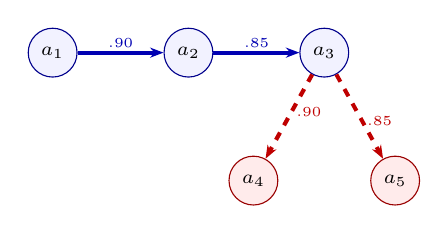
\begin{tikzpicture}[x=15mm, y=13mm]
  \node[atomtrue]  (a1) at (0,0)    {$a_1$};
  \node[atomtrue]  (a2) at (1.15,0) {$a_2$};
  \node[atomtrue]  (a3) at (2.3,0)  {$a_3$};
  \node[atomfalse] (a4) at (1.7,-1.25) {$a_4$};
  \node[atomfalse] (a5) at (2.9,-1.25) {$a_5$};

  \draw[ent,relw=0.90] (a1) -- (a2) node[wlab,above]{$.90$};
  \draw[ent,relw=0.85] (a2) -- (a3) node[wlab,above]{$.85$};
  \draw[con,relw=0.90] (a3) -- (a4) node[wlab,right,pos=0.45]{$.90$};
  \draw[con,relw=0.85] (a3) -- (a5) node[wlab,right,pos=0.55]{$.85$};
\end{tikzpicture}}
\caption{\textbf{A, coherent.} A support chain over the true claims; each false
  claim is attributed and then \emph{rejected} from $a_3$.
  $\LCS_{\mm}=0.590$.}
\label{fig:ex-a}
\end{subfigure}
\hfill
%% --- (b) Response B: the incoherent arrangement ---------------------------
\begin{subfigure}[b]{0.32\textwidth}
\centering
\resizebox{\linewidth}{!}{%
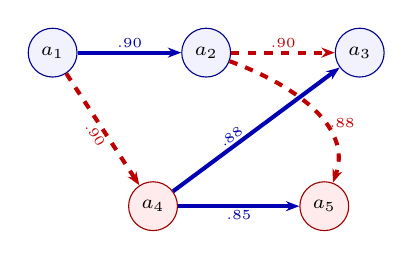
\begin{tikzpicture}[x=15mm, y=13mm]
  \node[atomtrue]  (a1) at (0,0)       {$a_1$};
  \node[atomtrue]  (a2) at (1.3,0)     {$a_2$};
  \node[atomtrue]  (a3) at (2.6,0)     {$a_3$};
  \node[atomfalse] (a4) at (0.85,-1.5) {$a_4$};
  \node[atomfalse] (a5) at (2.3,-1.5)  {$a_5$};

  \draw[ent,relw=0.90] (a1) -- (a2) node[wlab,above]{$.90$};
  \draw[con,relw=0.90] (a2) -- (a3) node[wlab,above]{$.90$};
  \draw[ent,relw=0.88] (a4) -- (a3) node[wlab,above,sloped,pos=0.38]{$.88$};
  \draw[con,relw=0.90] (a1) -- (a4) node[wlab,below,sloped]{$.90$};
  \draw[ent,relw=0.85] (a4) -- (a5) node[wlab,below]{$.85$};
  \draw[con,relw=0.88] (a2) to[out=-20,in=70]
        node[wlab,right,pos=0.62]{$.88$} (a5);
\end{tikzpicture}}
\caption{\textbf{B, incoherent.} The same five claims. $a_2\!\to\!a_3$ has become
  a conflict and the \emph{false} $a_4$ is now a premise for the true $a_3$.
  $\LCS_{\mm}=0.494$.}
\label{fig:ex-b}
\end{subfigure}
\hfill
%% --- (c) the MRF induced by (b) -------------------------------------------
\begin{subfigure}[b]{0.33\textwidth}
\centering
\resizebox{\linewidth}{!}{%
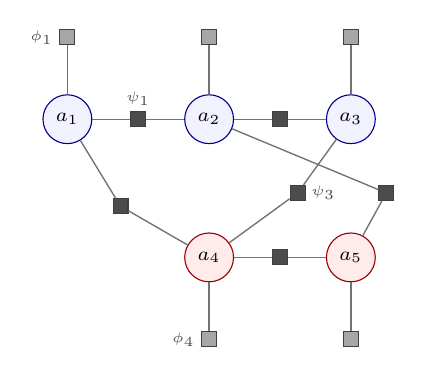
\begin{tikzpicture}[x=15mm, y=13mm]
  \node[atomtrue]  (a1) at (0,0)       {$a_1$};
  \node[atomtrue]  (a2) at (1.2,0)     {$a_2$};
  \node[atomtrue]  (a3) at (2.4,0)     {$a_3$};
  \node[atomfalse] (a4) at (1.2,-1.35) {$a_4$};
  \node[atomfalse] (a5) at (2.4,-1.35) {$a_5$};

  \node[unary] (p1) at (0,0.8)     {}; \draw[flink] (p1) -- (a1);
  \node[unary] (p2) at (1.2,0.8)   {}; \draw[flink] (p2) -- (a2);
  \node[unary] (p3) at (2.4,0.8)   {}; \draw[flink] (p3) -- (a3);
  \node[unary] (p4) at (1.2,-2.15) {}; \draw[flink] (p4) -- (a4);
  \node[unary] (p5) at (2.4,-2.15) {}; \draw[flink] (p5) -- (a5);
  \node[prlab,left=0.4mm of p1] {$\phi_1$};
  \node[prlab,left=0.4mm of p4] {$\phi_4$};

  \node[factor] (f12) at (0.6,0)      {}; \draw[flink] (a1) -- (f12) -- (a2);
  \node[factor] (f23) at (1.8,0)      {}; \draw[flink] (a2) -- (f23) -- (a3);
  \node[factor] (f43) at (1.95,-0.72) {}; \draw[flink] (a4) -- (f43) -- (a3);
  \node[factor] (f14) at (0.45,-0.85) {}; \draw[flink] (a1) -- (f14) -- (a4);
  \node[factor] (f45) at (1.8,-1.35)  {}; \draw[flink] (a4) -- (f45) -- (a5);
  \node[factor] (f25) at (2.7,-0.72)  {}; \draw[flink] (a2) -- (f25) -- (a5);
  \node[prlab,above=0.3mm of f12] {$\psi_1$};
  \node[prlab,right=0.3mm of f43] {$\psi_3$};
\end{tikzpicture}}
\caption{\textbf{The MRF of (b).} Grey squares are the unaries $\phi_i$ carrying
  the priors, black squares the pairwise $\psi_r$, one per relation.}
\label{fig:ex-mrf}
\end{subfigure}
\caption{The five-claim example of \S\ref{sec-example}. Blue nodes are claims true
  of the world ($\pi_i=0.9$), red nodes false ($\pi_i=0.1$); \emph{the same five
  claims appear in both graphs}, so every per-claim factuality check returns the
  same verdict on both responses. Solid blue edges are \ent{}, dashed red \con{};
  line width grows with the relation weight $p$. The unary factors $\phi_i$ of
  panel (c) are identical for the two responses, so the entire $0.590\to0.494$
  drop is produced by the pairwise $\psi_r$ --- by how the response arranges its
  claims, which is the whole of what coherence measures.}
\label{fig:example}
\end{figure}


Five claims about Voyager~1 are fixed once and for all, three true of the world (priors $0.9$) and two false
($0.1$): $a_1$, it crossed the heliopause in August 2012; $a_2$, after the crossing its instruments measured
a sharp rise in plasma density; $a_3$, it is therefore in interstellar space; and, false, $a_4$, its plasma
wave instrument failed permanently before the crossing, and $a_5$, it has left the Solar System entirely.

Two responses assert \emph{these same five claims} and differ only in how they arrange them, so every per-claim
factuality check returns the same verdict on both. \textbf{Response A} reports the density rise as what
established the crossing, concludes the probe is in interstellar space, then names the two false claims and
refuses each on a stated ground. \textbf{Response B} instead denies that the probe counts as being in
interstellar space, asserts the instrument failure as fact, offers \emph{that failure} as the reason the probe
reached interstellar space, chains it into having left the Solar System, and finally denies both falsehoods in
its closing sentence.

Figure~\ref{fig:example} shows the resulting graphs and the MRF that B induces. Two relation changes carry the
difference: the support edge $a_2\!\to\!a_3$ in A becomes a \con{} in B, which denies its own conclusion, and
the edge between $a_3$ and $a_4$ \emph{reverses} --- A rejects the false $a_4$ from $a_3$, while B makes $a_4$ a
premise \emph{for} $a_3$. Mentioning a falsehood is not what costs B its score; asserting it and reasoning from
it is. Exactly, by $2^5$ enumeration, A scores $\LCS_{\mm}=0.590$ against B's $0.494$: in A the true claims sit
at $0.939$, $0.989$ and $0.992$, each \emph{above} its $0.9$ prior because the chain supplies mutual support,
and the false ones at $0.013$ and $0.020$, whereas in B the \emph{true} $a_3$ is dragged to $0.513$ because its
only support arrives from $a_4$, which the response itself denies --- a premise the text refuses cannot transmit
support. The priors enter only through the unary $\phi_i$, identical in both responses, so the entire drop is
attributable to arrangement alone. App.~\ref{app-examples} gives both responses in full and two further
examples.

%% ================================================================
\section{The LoCoBench Benchmark}
\label{sec-locobench}
%% ================================================================

Validating a coherence measure requires responses that differ in coherence \emph{while holding content
fixed}, each accompanied by the relation graph a correct extractor would recover. Natural corpora supply
neither. They offer no controlled variation in coherence at constant claim content, so an observed score
difference cannot be attributed to coherence rather than to topic or length; and they carry no gold
relation graph, without which \emph{scoring} error cannot be separated from \emph{estimation} error --- the
one distinction our evaluation is built to make. We therefore evaluate on a synthesized corpus,
LoCoBench, and because the corpus is generated the burden is on us to state its construction completely.
This section does so: the object generated (\S\ref{sec-bench-ladder}), the pipeline that generates it
(\S\ref{sec-bench-pipeline}), how each rung's gold graph is derived (\S\ref{sec-bench-gold}), the
validation that gates admission (\S\ref{sec-bench-validation}), and what the released corpus contains
(\S\ref{sec-bench-corpus}).

\subsection{Coherence ladders}
\label{sec-bench-ladder}

\begin{definition}[Coherence ladder]
\label{def-ladder}
A \emph{ladder} is a tuple $(\mathcal{P},\langle\rho_0,\dots,\rho_4\rangle,\Gamma)$ in which
$\mathcal{P}$ is a base \emph{relation plan} --- a selected claim set together with a declared relation
graph over it --- each rung $\rho_k$ is a sequence of perturbation operator calls applied to
$\mathcal{P}$, realized as a response text and carrying \emph{its own} gold relation graph, and $\Gamma$
is a set of constraints on the relative ordering of the rungs' scores. A ladder is \emph{admitted} only
if all five rungs pass every validation gate of \S\ref{sec-bench-validation}.
\end{definition}

Two properties of Def.~\ref{def-ladder} carry the experimental design. First, all five rungs share one
claim set and one topic, so a measure that orders them is responding to relational structure and not to
content. Second, each rung carries its own gold graph rather than inheriting the base plan's, which is
what makes a rung a genuine test of a readout rather than a restatement of the corpus; \S\ref{sec-bench-gold}
gives the derivation.

\paragraph{Whole-family admission.} A ladder is admitted entire or rejected entire. Four of the five
rungs carry no standalone claim --- only a claim relative to their neighbours --- so a family missing a
rung is not a partial success but a broken comparison. A family whose fourth rung fails validation is
therefore rejected together with the four rungs that passed.

\begin{table}[tbp]
\centering\small
\caption{The four family types. Each holds the claim set, the topic and every unperturbed relation fixed,
  varying one structural dimension. \textsc{order} and \textsc{control} apply only meaning-preserving
  edits and so assert \emph{invariance}: \textsc{control} is the false-positive check, since a measure
  showing any monotone trend across it is tracking \emph{having been edited} rather than coherence. The
  final column is the count in the released corpus (\S\ref{sec-bench-corpus}).}
\label{tab:ladders}
\begin{tabular}{@{}lp{2.3cm}p{5.3cm}p{2.6cm}r@{}}
\toprule
Type & Dimension varied & Rungs, $\rho_0 \to \rho_4$ & Required pattern & $n$ \\
\midrule
\textsc{conflict} & conflict structure
  & \textsf{worse}, \textsf{base}, \textsf{concession\_resolved}, \textsf{fix\_one\_conflict},
    \textsf{coherent}
  & strictly increasing & 8 \\[3pt]
\textsc{chain} & entailment-chain integrity
  & \textsf{break\_3}, \textsf{break\_2}, \textsf{break\_1}, \textsf{base}, \textsf{coherent}
  & strictly increasing & 2 \\[3pt]
\textsc{order} & assertion order
  & \textsf{shuffle\_full}, \textsf{shuffle\_block}, \textsf{shuffle\_adjacent}, \textsf{base},
    \textsf{ordering\_only}
  & invariant & 3 \\[3pt]
\textsc{control} & nothing (meaning-preserving)
  & \textsf{ordering\_only}, \textsf{direction\_reversal}, \textsf{base},
    \textsf{direction\_reversal}, \textsf{ordering\_only}
  & flat throughout & 1 \\
\bottomrule
\end{tabular}
\end{table}

Table~\ref{tab:ladders} gives the four types, and the mix is load-bearing rather than incidental.
\textsc{conflict} is the reference ladder: only the conflict structure varies, which is what makes an
ordering attributable to coherence. \textsc{chain} tests a different failure mode --- breaking $N$ links
of an entailment chain and repairing them, so the defect is a \emph{missing} relation rather than a
present conflict. The distinction matters because a measure built on contradiction detection alone will
do well on the first ladder and fail the second. \textsc{order} and \textsc{control} are the negative
controls, and a corpus containing only increase-type ladders cannot distinguish a coherence measure from
an edit-count proxy: every rung of these two applies only meaning-preserving edits, so they assert that
the score does \emph{not} move. \S\ref{sec-ladder-results} reports that this is precisely where mined
relation graphs fail, a result no increasing-order ladder could have exposed.

\paragraph{Ordering constraints.} A family declares its constraints in three classes, asserted per
readout: \textbf{C1} a strict increase between consecutive rungs; \textbf{C2} a \emph{predicted} decrease
or invariance, which is where the concession dip of Prop.~\ref{prop-quirk} becomes falsifiable and where
an ordering-only edit must be exactly flat by Rem.~\ref{rem-order}; and \textbf{C3} endpoint separation
between $\rho_0$ and $\rho_4$. A missing score fails rather than passes. C2 is the only class that
predicts the internal behaviour of a particular readout, which is why the baseline comparison of
\S\ref{sec-baselines-measured} excludes it: a single-score baseline makes no claim a C2 constraint could
test.

\subsection{The generation pipeline}
\label{sec-bench-pipeline}

Generation is a five-stage prompted pipeline followed by validation. The stages are separated so that a
defect can be attributed to one of them and repaired there, and each stage's prompt is fixed and
versioned, with its numbered-instruction count and placeholder contract declared in
Table~\ref{tab:promptspec} and asserted by a test against the prompt strings themselves. The mechanism
matters because the alternative failure is silent: a corpus generated by prompts that no document
describes.

% The LoCoBench generation pipeline: five prompted stages, then three validators.
%
% Extracted from submit.tex so the figure has a single source and can be exported
% standalone by scripts/make_bench_pipeline_png.sh. The validators are V1, V3 and
% V4 by design -- those are the three that gate admission, and the numbering
% matches locobench/validate.py's threshold keys (v1_coupling, v1_sense,
% v3_min_score, v4_coverage). There is deliberately no V2 box.
%
% The committee that runs the validators EXCLUDES the generating model, which is
% why the two left-hand annotations name different model counts.
% ---------------------------------------------------------------------------
\begin{figure}[tbp]
\centering
\resizebox{\textwidth}{!}{%
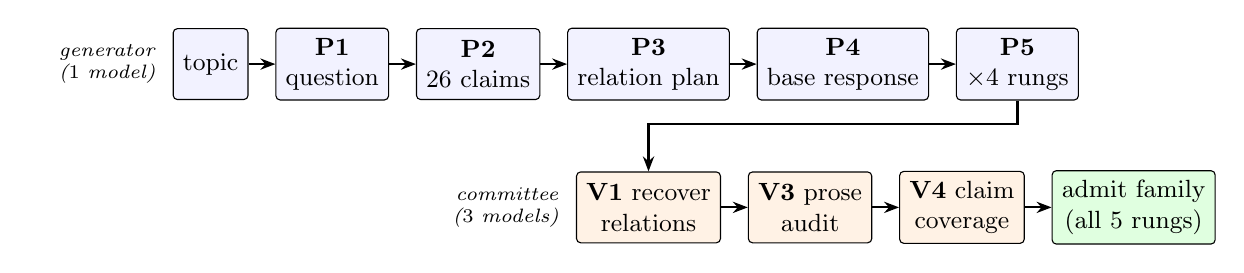
\begin{tikzpicture}[font=\small,
  st/.style={draw,rounded corners=1.5pt,align=center,inner sep=3.5pt,minimum height=9mm,fill=blue!5},
  vd/.style={draw,rounded corners=1.5pt,align=center,inner sep=3.5pt,minimum height=9mm,fill=orange!10},
  fin/.style={draw,rounded corners=1.5pt,align=center,inner sep=3.5pt,minimum height=9mm,fill=green!12},
  ar/.style={-{Stealth[length=1.9mm]},thick}, node distance=3.4mm]
  \node[st] (t) {topic};
  \node[st,right=of t] (p1) {\textbf{P1}\\question};
  \node[st,right=of p1] (p2) {\textbf{P2}\\$26$ claims};
  \node[st,right=of p2] (p3) {\textbf{P3}\\relation plan};
  \node[st,right=of p3] (p4) {\textbf{P4}\\base response};
  \node[st,right=of p4] (p5) {\textbf{P5}\\$\times 4$ rungs};
  \foreach \a/\b in {t/p1,p1/p2,p2/p3,p3/p4,p4/p5} \draw[ar] (\a) -- (\b);
  \node[vd,below=9mm of p3] (v1) {\textbf{V1} recover\\relations};
  \node[vd,right=of v1] (v3) {\textbf{V3} prose\\audit};
  \node[vd,right=of v3] (v4) {\textbf{V4} claim\\coverage};
  \node[fin,right=of v4] (adm) {admit family\\(all $5$ rungs)};
  \draw[ar] (p5.south) -- ++(0,-3mm) -| (v1.north);
  \draw[ar] (v1) -- (v3); \draw[ar] (v3) -- (v4); \draw[ar] (v4) -- (adm);
  \node[left=1mm of v1,font=\scriptsize\itshape,align=right,text width=15mm] {committee\\($3$ models)};
  \node[left=1mm of t,font=\scriptsize\itshape,align=right,text width=15mm] {generator\\($1$ model)};
\end{tikzpicture}}
% scripts/make_bench_pipeline_png.sh defines \bpnocaption to render this figure
% for standalone export, where surrounding prose supplies the explanation.
% Undefined in the paper, so the caption below is typeset normally there.
\ifdefined\bpnocaption\else
\caption{The generation pipeline. Five stages produce a family of five rungs from one topic; three
  validators, run by a committee that \emph{excludes} the generating model, gate admission. A family is
  admitted whole or rejected whole (Def.~\ref{def-ladder}).}
\label{fig:bench-pipeline}
\fi
\end{figure}


The five stages, in order (Fig.~\ref{fig:bench-pipeline}), are as follows.

\textbf{P1: topic to question.} Given a topic from an inventory of $36$ topics across four domains, emit
one open-ended question. The prompt enumerates the target relations, so the question is chosen with the
downstream plan in mind rather than for topical interest, and it prefers adjudicative domains ---
incident investigations, litigation, diagnostic reasoning, attribution disputes, competing hypotheses ---
because those are the settings in which exhaustive alternatives and resolving holdings arise naturally.

\textbf{P2: question to claims.} Emit $26$ atomic claims answering the question, each a single
proposition, tagged with a truth status. A surplus is generated deliberately: P3 selects a subset, and
selection from a surplus is what lets the plan choose claims that support the required relation structure
instead of forcing relations onto whatever claims exist.

\textbf{P3: claims to relation plan.} Select $14$--$16$ claims (aiming for $15$) and plan exactly $10$
relations over them using the two-level scheme of \S\ref{sec-levels}, with at least one relation of each
required sense, together with $4$--$6$ pairs \emph{explicitly declared unrelated}. Relations are kept
local, preferring pairs within four positions, which is what makes a windowed candidate policy a
reasonable baseline rather than a straw man. The declared non-relations are the corpus's labelled negative
set, and they are what makes a precision figure meaningful: precision against ``every pair not in gold''
is dominated by unlabelled pairs of unknown status, whereas precision against pairs the item asserts are
unrelated is a real number. Each relation also carries an intended strength band and an intended
\emph{validity} --- valid when the relation genuinely holds, invalid when the prose draws it unsoundly ---
targeting a valid fraction near $0.55$, so a scorer cannot succeed by assuming every relation it finds is
sound. The shipped items carry $7$--$11$ relations each and $2$--$3$ false claims, the spread arising
because a rung's perturbations add and remove edges relative to the plan.

\textbf{P4: plan to response.} Realize the plan as continuous prose of $550$--$650$ words, asserting
every selected claim and drawing every planned relation, with no headings or lists. The floor exceeds
the default completion-token grant of some gateways; a model that hits the cap returns prose stopped
mid-sentence, which every parser rejects but for the wrong stated reason, so the ceiling is raised
explicitly rather than left to the backend default.

\textbf{P5: response to rung.} Apply exactly one perturbation to the base response, changing the minimum
number of words and preserving everything else verbatim. Table~\ref{tab:operators} gives the six
operators and the ten parameterized calls realizing them. The stage also emits a structured diff naming
the operator, its target, the sentences changed and the relations added, removed or relabelled; length
drift is capped at $15\%$ except for the three calls that add or remove a sentence by definition.

\begin{table}[tbp]
\centering\small
\caption{The six perturbation operators and the ten calls realizing them. Each call has a declared effect
  on the rung's \emph{gold relation graph} as well as on its text, which is what makes
  \S\ref{sec-bench-gold}'s derivation well defined. The two \textsc{o6} calls are factor-invariant by
  design: they are what the \textsc{order} and \textsc{control} ladders exist to check.}
\label{tab:operators}
\begin{tabular}{@{}lp{3.1cm}p{7.6cm}@{}}
\toprule
Op & Calls & Effect on the text \\
\midrule
\textsc{o1} relabel & \textsf{wrong\_sense}, \textsf{direction\_reversal},
  \textsf{exhaustiveness\_flip}
  & rewrite the connective so the text draws a different sense, reverses the relation, or flips
    \sense{Contrast}$\leftrightarrow$\sense{Alternative} \\
\textsc{o2} add conflict & \textsf{inject\_contradiction}, \textsf{spurious\_relation}
  & add one sentence directly contradicting a named claim, at least two sentences later; or assert a
    link between two claims the response kept separate \\
\textsc{o3} break chain & \textsf{break\_chain}
  & remove or negate the link realizing an edge so the chain no longer connects, keeping both
    endpoints \\
\textsc{o4} drop relation & \textsf{drop\_relation}
  & remove the connective realizing an edge, leaving the two claims as adjacent assertions \\
\textsc{o5} resolve & \textsf{add\_resolution}, \textsf{remove\_resolution}
  & add or delete the holding sentence that settles a conceded tension \\
\textsc{o6} reorder & \textsf{shuffle\_order}, \textsf{ordering\_only}
  & permute sentences at full, block or adjacent granularity; or exchange
    \sense{Precedence}$\leftrightarrow$\sense{Succession} preserving chronology ---
    \emph{no coupling changes} \\
\bottomrule
\end{tabular}
\end{table}

\begin{table}[tbp]
\centering\small
\caption{Prompt specification. Each prompt's numbered-instruction count and required placeholder set are
  declared here and asserted by a test against the prompt strings, so a prompt cannot drift from the
  document describing it without the test failing. Instructions are counted by matching lines beginning
  at column one with a digit, period and space, so indented sub-items --- P3's per-sense glosses, P5's
  per-call definitions --- do not inflate the count. The validators carry no numbered instructions
  because their prompts specify an output schema rather than a procedure.}
\label{tab:promptspec}
\begin{tabular}{@{}llrl@{}}
\toprule
Stage & Role & Instructions & Required placeholders \\
\midrule
P1 & topic $\to$ question        & $9$  & \texttt{TOPIC} \\
P2 & question $\to$ claims       & $7$  & \texttt{QUESTION} \\
P3 & claims $\to$ relation plan  & $10$ & \texttt{CLAIMS}, \texttt{QUESTION} \\
P4 & plan $\to$ base response    & $8$  & \texttt{PLAN}, \texttt{QUESTION} \\
P5 & response $\to$ rung         & $5$  & \texttt{OPERATOR}, \texttt{PLAN}, \texttt{RESPONSE} \\
\midrule
V1 & recover relations           & $0$  & \texttt{ATOMS}, \texttt{RESPONSE} \\
V3 & prose audit                 & $0$  & \texttt{RESPONSE} \\
V4 & claim coverage              & $0$  & \texttt{ATOMS}, \texttt{RESPONSE} \\
\bottomrule
\end{tabular}
\end{table}

\paragraph{The failure policy.} What happens when a stage's output is defective is a specification
decision, and the policy is per stage with four outcomes. A \textbf{retry} handles a transient parse
failure where the inputs are sound; because a byte-identical prompt re-sent to a temperature-zero backend
cannot produce a different parse, retries are issued at successively higher sampling temperatures, which
is what makes a retry budget worth more than one attempt. A \textbf{regenerate} handles an artifact that
is wrong while its inputs are fine. A \textbf{drop edge} applies to V1 alone: an unrecovered relation
must never be retained as gold, since gold the prose does not realize is exactly the defect that gate
exists to catch. A \textbf{reject} applies when a family cannot carry its ranking claim, and stores the
family with its reason rather than discarding it, so rejection rates remain auditable.

\subsection{Deriving each rung's gold relation graph}
\label{sec-bench-gold}

A rung's gold graph is the base plan's graph with that rung's operator calls applied. Three mechanisms
make this well defined, and each closes a way the derivation could otherwise produce a rung that does not
match its own prose.

\emph{Target assignment.} Each call in a rung is assigned a distinct eligible edge, so a rung composing
two \textsf{drop\_relation} calls drops two \emph{different} edges. Eligibility is call-dependent: a
\textsf{drop\_relation} in a conflict ladder targets an unresolved conflict edge, an
\textsf{add\_resolution} a resolvable one. A \textsc{conflict} plan therefore needs three unresolved
conflict edges to support its full ladder --- one for the resolution and two for the drops --- and a plan
with fewer is rejected at generation time rather than silently emitting a rung that duplicates its
neighbour.

\emph{Derived-field re-derivation.} When a call changes an edge's sense, the coupling, directedness,
ordering-only status and exhaustiveness are re-derived from the new sense through the compile map
$\mathcal{C}$ rather than carried over, so a transformed edge cannot contradict $\mathcal{C}$.

\emph{The adjacency gate.} A family is rejected when two \emph{adjacent} rungs build the same edge set
while the higher rung's calls claim a change. Adjacency rather than parentage is the right comparison:
every \textsc{conflict} rung declares the base as its parent, so a parent-only check passes a rung that
duplicates the rung immediately below it. The two factor-invariant calls of \textsc{o6} are exempt, since
they are \emph{intended} to leave the edge set unchanged --- which is exactly what makes them usable as
invariance tests.

\subsection{Validation}
\label{sec-bench-validation}

An item is admitted only if an independent committee certifies it, and three properties of the
arrangement matter more than the individual gates.

\textbf{The committee excludes the generator.} Validation is run by a panel of models, and the model that
generated a family is removed from its own panel before voting. Without this, the dominant failure mode of
an LLM-generated benchmark --- the generator certifying its own idiosyncrasies as ground truth --- is
structurally unaddressed. Each gate is decided by \emph{majority} of the remaining panel, and a facet
counts as failed only when a majority objects, so one unusually strict auditor cannot reject a sound
family.

\textbf{Every threshold lives in one place.} All acceptance thresholds are declared in
Table~\ref{tab:thresholds} and nowhere else. A benchmark whose thresholds are scattered across the code
applying them cannot be replicated from its description, nor re-run at a different operating point
without a search for the constants.

\textbf{Generation is rejected, never repaired.} A family failing a gate is stored with its reason and
discarded. No stage patches a defective artifact into an acceptable one, because a repaired item's gold
labels no longer describe a process we can state.

\begin{table}[tbp]
\centering\small
\caption{Every acceptance threshold. V1 rates are computed over the \emph{valid} planned relations only,
  since an invalid planned relation is one the prose is not required to draw soundly. The rightmost
  column is the committee decision rule for that gate.}
\label{tab:thresholds}
\begin{tabular}{@{}llll@{}}
\toprule
Gate & Quantity & Threshold & Rule \\
\midrule
V1 & planned relations recovered with correct coupling & $\ge 0.80$ & majority \\
V1 & \dots\ and with correct sense & $\ge 0.70$ & majority \\
V3 & fluency, formality, organization (each, of $5$) & $\ge 4$ & majority \\
V3 & leakage and hedging span lists & must be empty & majority \\
V4 & claim coverage over gating statuses & $=1.00$ & majority \\
\midrule
P3 & claims selected & $14$--$16$ & --- \\
P3 & relations planned (accepted band; $10$ instructed) & $8$--$12$ & --- \\
P3 & declared non-relations & $4$--$6$ & --- \\
P3 & fraction of relations valid & $0.55 \pm 0.15$ & --- \\
P3 & false claims selected & $\ge 2$ & --- \\
P5 & length drift & $\le 15\%$ & --- \\
\bottomrule
\end{tabular}
\end{table}

The three gates test different things. \textbf{V1}, the load-bearing one, hands an independent model the
response and its claims and asks it to recover the relations the response \emph{itself} draws, emitting
for each ordered pair a sense, a coupling, a strength band and a resolved flag; admission requires
$\ge 0.80$ of valid planned relations returned with the correct coupling and $\ge 0.70$ with the correct
sense. This is what certifies that the gold graph describes the prose rather than the plan, and it is the
gate that makes the \textsc{gold} relation source of \S\ref{sec-protocol} meaningful. \textbf{V3} audits the prose
for fluency, formality and organization, and requires the leakage and hedging span lists to be empty ---
leakage being any text that names the annotation scheme or the perturbation, which would let a scorer
detect the rung without reading for coherence. \textbf{V4} checks that every selected claim is actually
asserted, gating on the \textsf{missing} and \textsf{merged} statuses, since a claim the response never
makes cannot stand in a relation.

\subsection{The released corpus}
\label{sec-bench-corpus}

\begin{table}[tbp]
\centering\small
\caption{Composition of the released corpus. Every figure is computed from the shipped items rather than
  from the generation targets. \emph{Edge-producing} excludes the $67$ ordering-only relations, which
  compile to \coupling{none} and contribute no factor; \emph{backward} counts edge-producing relations
  whose target precedes its source in assertion order, the relations a forward-only candidate policy
  cannot reach (\S\ref{sec-bottleneck}).}
\label{tab:corpus}
\begin{tabular}{@{}lr@{\qquad}lr@{}}
\toprule
Quantity & Value & Quantity & Value \\
\midrule
Families              & $14$   & Gold relations, total            & $670$ \\
Items (rungs)         & $70$   & \quad edge-producing             & $603$ \\
Claims                & $1{,}115$ & \quad valid                   & $408$ \quad ($0.61$) \\
Claims per item       & $15$--$16$ & \quad backward                & $105$ \\
Words per item        & $609$--$698$ & Declared non-relations      & $342$ \\
Distinct topics       & $14$   & Ordering constraints per source     & $202$ \\
\midrule
\textsc{conflict} / \textsc{chain} & $8$ / $2$ & C1 / C2 / C3 checks & $112$ / $30$ / $45$\,+\,$15$ \\
\textsc{order} / \textsc{control}  & $3$ / $1$ & Generator / committee & $1$ / $3$ models \\
\bottomrule
\end{tabular}
\end{table}

Table~\ref{tab:corpus} states what the corpus contains. It was produced by \texttt{claude-opus-5} and
admitted by a three-model cross-vendor committee (\texttt{gpt-5.6-terra}, \texttt{gemini-3.1-pro},
\texttt{claude-sonnet-5}), none of which is the generator. The $14$ families cover $14$ distinct topics
spanning all four domains --- four Natural Sciences, four Engineering \& Technology, three Humanities,
three Social Sciences --- so no single topic or domain carries a result. All four family types are
represented, which is what allows \S\ref{sec-ladder-results} to report the increase and invariance axes
separately; the $202$ ordering constraints decompose as $112$ over \textsc{conflict}, $30$ over
\textsc{chain}, $45$ over \textsc{order} and $15$ over \textsc{control}.

Two properties of the corpus bound what can be concluded from it, and we state them here rather than in
the limitations so that the results below are read correctly. It is LLM-generated throughout, so an
idiosyncrasy shared by the generator and all three validators would be invisible to this construction.
And at $70$ items it is small in absolute terms: the per-source comparisons of \S\ref{sec-ladder-results}
rest on $202$ assertions, which is enough to separate sources differing by tens of points but not enough to
resolve differences of a few.

%% ================================================================
\section{Experiments}
\label{sec-experiments}
%% ================================================================

The measure of \S\ref{sec-coherence} has two components that can fail independently: the probabilistic model, and
the estimator that supplies its relation graph. An evaluation conflating them cannot say which to fix, so our
experiments are built around one device --- holding the readouts byte-identical and swapping only the relation
graph (\S\ref{sec-protocol}) --- which attributes any shortfall to one component or the other by construction. We
then ask three questions in turn: how accurate is the estimator (\S\ref{sec-bottleneck}), how well does the model
order responses given a correct graph (\S\ref{sec-ladder-results}), and how does the measure compare against
evidence-free alternatives (\S\ref{sec-baselines-measured}). \S\ref{sec-summary} draws the answers together and
\S\ref{sec-limitations} bounds them.

\subsection{Protocol}
\label{sec-protocol}

A \emph{relation source} fixes where the relation graph comes from while holding claims, priors, readouts and scorer
settings byte-identical --- the central experimental device of the paper. \textsc{gold} takes each item's own
labelled relations, \textsc{gold\_valid} only those labelled valid, and a \textsc{mined} source runs the estimator
of \S\ref{sec-mining} on the response text; because the readouts are identical across sources, any shortfall below
gold is attributable to relation estimation and not to the probabilistic model. Mined relations are compared to
gold at three nested levels, defined with the measurement in \S\ref{sec-bottleneck}.

The corpus is the one specified in \S\ref{sec-locobench}: $14$ families, $70$ items, $1{,}115$ claims and
$670$ gold relations, declaring $202$ ordering constraints per source (Table~\ref{tab:corpus}). Mining is sampled
once per cell rather than averaged, so we measure the resulting variability instead of estimating it: two
\emph{independent} runs of the same configurations moved every pair, coupling and sense F1 by at most $0.014$,
while the gold sources reproduced bit-for-bit. Per-source ladder agreement is the noisier statistic, moving by four to
six of $202$ assertions between those runs, so a single source's percentage should not be read to the point and
differences below roughly six assertions are not resolvable here. Exact values are by $2^{16}$ enumeration,
corpus-scale ones by weighted mini-bucket \citep{wmb} at i-bound $6$.

Five baseline families are chosen to fail in informative ways; four are implemented and share the LCS's own
decomposition, so each sees the same atoms and no retrieved evidence: ladder-blind controls (claim count,
relation count, length) that catch a measure secretly tracking edit count or graph density
\citep{steenmarkert}; pairwise NLI with no global model \citep{selfcheckgpt}; ROSCOE's Self-Consistency
\citep{roscoe} in max, mean and symmetric variants; LLM judges --- G-Eval \citep{geval} with the SummEval
rubric \citep{summeval} and a direct rating prompt, each a mean over five runs; and the three single-document
DiscoScore metrics \citep{discoscore} with an entity grid \citep{barzilay}.

\subsection{Relation estimation is the bottleneck}
\label{sec-bottleneck}

We begin with the estimator, since every mined relation source inherits its errors. Measuring it against gold separates a
model that scores a graph badly from an extractor that supplies the wrong graph.

\begin{table}[tbp]
\centering\small
\caption{Mined-versus-gold agreement, micro-averaged over the seventy items. The denominator is the
  $603$ \emph{edge-producing} gold relations ($670$ total, less the $67$ ordering-only edges, which
  compile to \coupling{none} and contribute no factor). Agreement is scored at three increasingly
  strict levels: recovering the \textbf{pair}, then its \textbf{coupling} (which selects the factor
  table), then its \textbf{sense}. \textbf{By direction} decomposes coupling recall according to
  whether the gold relation runs forward or backward in assertion order --- $105$ of the $603$ run
  backward, and no forward-only candidate set can reach them. \textbf{Errors} counts violations of
  the $342$ declared-unrelated pairs (\textbf{non-rel}) and unordered pairs receiving two factors
  (\textbf{dup}). All figures are percentages except the three counts (edges, non-rel, dup).
  \textbf{Bold marks the best F1, not the best recall}: \textsc{bidirectional} wins every recall
  column under either miner and is nonetheless the weaker policy, which is the trade-off this table
  exists to show.}
\label{tab:mining}
% Layout follows Table tab:ladder: the miner is an italic banner row spanning the table
% rather than a column, so the model can be named in full without paying column width for
% it, and the policy keeps its own column. Metric families are \cmidrule-grouped so that
% "recall by direction" reads as a decomposition of coupling recall; emphasis is on F1 only
% (see the caption). tabcolsep is trimmed because twelve numeric columns pay for it twice
% each, and at 5.5in the group HEADERS, not the data, are the binding constraint.
\setlength{\tabcolsep}{2.5pt}
\begin{tabular}{@{}l@{\hspace{7pt}}r@{\hspace{6pt}}rrr@{\hspace{6pt}}rrr@{\hspace{6pt}}r@{\hspace{6pt}}rr@{\hspace{6pt}}rr@{}}
\toprule
 & & \multicolumn{3}{c@{\hspace{6pt}}}{Pair} & \multicolumn{3}{c@{\hspace{6pt}}}{Coupling}
 & Sense & \multicolumn{2}{c@{\hspace{6pt}}}{Recall by dir.} & \multicolumn{2}{c}{Errors} \\
\cmidrule(r{5pt}){3-5}\cmidrule(r{5pt}){6-8}\cmidrule(r{5pt}){9-9}\cmidrule(r{5pt}){10-11}\cmidrule(r){12-13}
Policy & Edges & P & R & F1 & P & R & F1 & F1 & fwd & bwd & non-rel & dup \\
\midrule
\multicolumn{13}{@{}l}{\emph{mined by} \texttt{llama-3.3-70b}} \\
\textsc{windowed}      & $1{,}106$ & $44.8$ & $82.3$ & $58.0$ & $34.1$ & $62.5$ & $44.1$ & $37.6$ & $71.1$ & $21.9$ & $34$ & $0$ \\
\textsc{bidirectional} & $3{,}172$ & $28.5$ & $91.7$ & $43.5$ & $17.9$ & $79.3$ & $29.3$ & $24.7$ & $79.9$ & $76.2$ & $119$ & $1{,}231$ \\
\multicolumn{13}{@{}l}{\emph{mined by} \texttt{gpt-oss-120b}} \\
\textsc{windowed}      & $1{,}094$ & $46.0$ & $83.4$ & $59.3$ & $40.2$ & $73.0$ & $\mathbf{51.9}$ & $\mathbf{47.0}$ & $82.1$ & $29.5$ & $38$ & $0$ \\
\textsc{bidirectional} & $2{,}973$ & $29.8$ & $96.5$ & $45.5$ & $22.4$ & $88.4$ & $35.8$ & $32.3$ & $89.0$ & $85.7$ & $147$ & $1{,}020$ \\
\bottomrule
\end{tabular}
\end{table}

\paragraph{How the numbers were obtained.} Each source of Table~\ref{tab:mining} is one miner paired with one
candidate-pair policy, run over the same seventy items. The policy fixes which claim pairs the miner is ever
asked about, and the two differ structurally rather than by degree: \textsc{windowed} proposes only
\emph{forward} arcs within an order radius of $w=4$ (source before target in assertion order), yielding $1{,}693$
candidate pairs over the corpus, while \textsc{bidirectional} proposes \emph{both} arcs of every pair and applies
no window, yielding $7{,}520$ --- a $4.4\times$ larger question set from identical inputs. Each surviving
candidate then costs two LLM calls, Prompt A for the discourse sense and its coupling and Prompt B for the
conditional strength (App.~\ref{app-mining}); the measured rate is $1.65$ calls per pair under \textsc{windowed}
and $1.41$ under \textsc{bidirectional}, below two because Prompt B is skipped whenever Prompt A returns
\sense{none} --- which it does for $593$ and $4{,}447$ pairs respectively. We then compare the surviving
relations to the item's gold graph at three \emph{nested} levels, because they answer different questions:
\textbf{pair} asks only whether the miner saw the two claims as related at all, isolating candidate selection
from labelling; \textbf{coupling} additionally requires the correct Level-1 coupling, which is the headline
because the coupling is what selects the factor table; and \textbf{sense} additionally requires the Level-2
discourse sense, which diagnoses taxonomy confusion rather than anything the MRF does. A mined edge matches a
gold one on the \emph{ordered} pair when the coupling is asymmetric, where direction is part of the claim, and on
the \emph{unordered} pair when it is symmetric, where scoring direction would charge a policy's arc ordering as a
labelling error. Counts are micro-averaged over the seventy items against the $603$ edge-producing gold
relations.

\paragraph{What they mean.} The decomposition matters more than any single F1, because it says \emph{which} step
fails. Take \texttt{llama-3.3-70b} under \textsc{windowed}: of the $603$ gold relations it finds $496$ as pairs,
types $377$ of those with the right coupling, and gets the sense right on $321$. So the estimator is not mostly
failing to notice that two claims are related --- it recovers four fifths of the pairs --- it is failing to
\emph{type} what it found, losing $119$ relations to the wrong coupling and $56$ more to the wrong sense. That is
what makes ``extraction is the bottleneck'' a claim about labelling rather than about recall, and it is why
coupling F1, not pair F1, is the column to read. The second half of the story is precision. The same source emits
$729$ spurious couplings against its $377$ correct ones, and under \textsc{bidirectional} that becomes $2{,}187$
against $478$. Because Eq.~\ref{eq-joint} is a \emph{product} over relations, a spurious factor is not a diluted
signal but an active one pulling marginals toward the prior, so precision is not tradeable against recall here in
the way an F1 suggests; the $1{,}231$ duplicate unordered pairs are the same defect seen structurally --- two
factors on one variable pair, which the model has no principled way to combine --- and declared-non-relation
violations rise from $34/342$ to $119/342$ in step. The two effects together explain the table's central
inversion. Forward-only mining is \emph{structurally} capped, reaching $21.9$--$29.5\%$ of backward-running gold
relations against $76.2$--$85.7\%$ for \textsc{bidirectional}, because $105$ of the $603$ relations run backward
and no forward-only candidate set can emit them; but buying that reach costs more in precision than it returns in
recall, so coupling F1 \emph{falls} from $44.1$ to $29.3$. Reach and accuracy are separate axes, and on this
corpus the wider policy is the weaker one. Finally, \texttt{gpt-oss-120b} is the better miner at every level ---
by $7.7$ points of coupling F1, $9.5$ of sense F1 and $7.6$ of backward recall under \textsc{windowed}, while
emitting slightly \emph{fewer} edges --- but it is also the less informative one: $99\%$ of its strength
estimates sit at a clamp boundary against $59\%$ interior for \texttt{llama}, and it returns just nine distinct
strength values across $1{,}094$ relations against \texttt{llama}'s $600$. It decides confidently and supplies
almost no graded uncertainty for the model to use.

\subsection{The model orders correctly when the graph is correct}
\label{sec-ladder-results}

Holding the readouts fixed and varying only the graph now isolates the model's own behaviour.

\begin{table}[tbp]
\centering\small
\caption{\textbf{Left:} declared ordering constraints satisfied, by ladder type --- $202$ assertions
  per source. \textsc{order} and \textsc{control} assert \emph{invariance}, so a readout that trends
  there is tracking surface form rather than coherence; \textsc{gold\_valid} is near-flat on
  \textsc{conflict} by construction, so its failures carry no information about the readouts and the
  \textsc{gold} source is what the constraints test. \textbf{Right:} each readout's mean over the seventy
  items, with the standard deviation in grey. Averaging across a ladder's rungs \emph{deliberately
  collapses the ordering the ladder exists to test}, so the right-hand block is a \textbf{level
  comparison only} and carries no evidence about ordering --- that is entirely the left block's job;
  the spreads are given because a mean alone cannot say whether a source is stable or merely
  centred. The reified readout is omitted here; App.~\ref{app-readouts} compares all four.}
\label{tab:ladder}
% The Source and Policy columns were mutually exclusive (gold rows have no policy, mined rows no source
% name -- the banner rows carry the miner), so they are merged into one. That pays for the
% standard deviations, which cost ~23pt per readout cell: measured 377pt against a 397pt line.
\setlength{\tabcolsep}{2.5pt}
\begin{tabular}{@{}l@{\hspace{7pt}}rrrrr@{\hspace{9pt}}rrr@{}}
\toprule
& \multicolumn{5}{c@{\hspace{9pt}}}{Constraints satisfied} & \multicolumn{3}{c}{Mean readout value (sd)} \\
\cmidrule(r{8pt}){2-6}\cmidrule(l){7-9}
Source / policy & Cfl & Chn & Ord & Ctl & \% & $\LCS_{\mm}$ & $\LCS_{\cons}$ & $\LCS_{\lp}$ \\
\midrule
\textsc{gold}        & 89/112 & 18/30 & 45/45 & 15/15 & \textbf{82.7} & $0.795$\pmsd{0.022} & $0.515$\pmsd{0.135} & $0.410$\pmsd{0.090} \\
\textsc{gold\_valid} & 37/112 & 12/30 & 45/45 & 15/15 & 54.0 & $0.794$\pmsd{0.020} & $0.576$\pmsd{0.151} & $0.485$\pmsd{0.047} \\
\midrule
\multicolumn{9}{@{}l}{\emph{mined by} \texttt{llama-3.3-70b}} \\
\textsc{windowed}      & 53/112 & 17/30 & 0/45 & 0/15 & 34.7 & $0.796$\pmsd{0.089} & $0.676$\pmsd{0.239} & $0.224$\pmsd{0.158} \\
\textsc{bidirectional} & 57/112 & 18/30 & 0/45 & 0/15 & 37.1 & $0.723$\pmsd{0.171} & $0.542$\pmsd{0.196} & $0.037$\pmsd{0.026} \\
\multicolumn{9}{@{}l}{\emph{mined by} \texttt{gpt-oss-120b}} \\
\textsc{windowed}      & 59/112 & 12/30 & 0/45 & 0/15 & 35.1 & $0.825$\pmsd{0.074} & $0.500$\pmsd{0.138} & $0.129$\pmsd{0.096} \\
\textsc{bidirectional} & 53/112 & 17/30 & 0/45 & 0/15 & 34.7 & $0.808$\pmsd{0.128} & $0.462$\pmsd{0.095} & $0.033$\pmsd{0.059} \\
\bottomrule
\end{tabular}
\end{table}

\paragraph{How a constraint is scored.} A \emph{relation source} fixes only where the relation graph comes from;
the claims, the priors, the readouts and every scorer setting are byte-identical across sources
(\S\ref{sec-protocol}), so any difference between two rows of Table~\ref{tab:ladder} is caused by the
graph and nothing else. A single \emph{constraint} is one assertion about one readout on one pair of
rungs: we score both rungs, take the difference, and ask whether it has the declared sign, counting a
difference below $10^{-6}$ as flat. The assertions come in three classes --- \textbf{C1} a strict
increase between consecutive rungs ($96$ of them), \textbf{C2} a \emph{predicted} decrease or exact
flatness ($64$), and \textbf{C3} separation between the first and last rung ($42$) --- for $202$ per
source, distributed over the four ladder types as the table's columns show. The percentage is simply the
fraction satisfied, and a missing score counts as a failure rather than being skipped. Because a
constraint is a claim about a \emph{difference}, the left-hand block of Table~\ref{tab:ladder} is the
only part that tests ordering; the mean readout values on the right average that difference away by
construction and are reported for level comparison alone.

On gold relations the readouts satisfy $82.7\%$ of these constraints --- $167$ of $202$ --- against
$34.7$--$37.1\%$ for every mined source. Since sources differ only in the graph, that $46$--$48$ point gap is
attributable to relation estimation alone, and its size is what §\ref{sec-bottleneck} predicts: at
$29$--$52\%$ coupling F1 roughly half the factors in a mined network are wrong or missing, and a ladder
whose consecutive rungs differ by one or two relations cannot survive that. This is the paper's central
empirical claim, and it is a claim about \emph{where} the remaining problem is --- the probabilistic
model orders responses correctly when handed a correct graph, and extracting one is the open problem.

The per-ladder breakdown localizes the failure. On gold, \textsc{order} and \textsc{control} are perfect
($45/45$, $15/15$) since those rungs move no factor, \textsc{conflict} is strong at $89/112$, and \textsc{chain}
the weak ladder at $18/30$. But \emph{every mined source scores $0/45$ on \textsc{order} and $0/15$ on
\textsc{control}} --- the most consequential number in the table, and not a scoring artefact: those ladders hold
the claim set fixed and permute the prose, yet on one \textsc{order} family the \texttt{gpt-oss}
\textsc{windowed} miner emitted $9$, $16$, $20$, $20$ and $17$ edges across five rungs differing \emph{only} in
sentence order. LLM relation extraction is therefore not reorder-invariant, and any measure built on it inherits
that sensitivity however sound its probabilistic layer. Mined sources are nonetheless \emph{not} uniformly worse
(\textsc{conflict} $53$--$59$ of $112$, \textsc{chain} $12$--$18$ of $30$), so a measure evaluated only on
increase-type ladders would have called mined extraction far closer to gold than it is --- precisely the false
positive the \textsc{control} ladder was added to catch. Mined ladder agreement also does \emph{not} track coupling
F1 --- \texttt{llama}'s \textsc{bidirectional} source has the worst coupling F1 ($29.3$) and the best agreement
($37.1\%$) --- so these sources are not separated by ladder agreement at all, and candidate policies should not be
ranked on it.

\subsection{What the baselines are}
\label{sec-baselines-what}

Table~\ref{tab:summary-mined} sets the LCS against ten baseline columns, and reading it needs to know what
each one computes. All are evidence-free and all consume the LCS's own atom decomposition, so every
row sees the same claims and no retrieved passages; the only thing varying across the table is how a
measure turns those claims into a number. App.~\ref{app-protocol} gives the design rationale --- why
each family is chosen to fail informatively rather than to be a weak competitor --- and what follows
is the operational content.

\paragraph{Discourse representations (\textsc{rc}, \textsc{lc}, \textsc{entity graph}).} Three
single-document metrics from DiscoScore \citep{discoscore}. DiscoScore is presented as
reference-based and most of its variants consume a reference a standalone response does not have;
these three ignore the reference argument entirely, and the last \emph{is} an entity grid
\citep{barzilay}, so the classical baseline comes from the same implementation. \textsc{rc} is
repeated noun mentions over distinct nouns; \textsc{lc} is nouns occurring in more than one sentence
over distinct nouns; \textsc{entity graph} is the mean sentence-adjacency weight, an edge of weight
$1/(j-i)$ wherever sentences $i$ and $j$ share a noun lemma. All three therefore reduce to
noun-lemma repetition, with no representation of entailment, relation type or contradiction. A
response can contradict itself in every sentence and still score at ceiling provided its nouns
recur, which is what makes them a test of whether coherence is separable from \emph{cohesion} rather
than a weak competitor --- and \textsc{rc} is nonetheless the strongest baseline in the table at
$30/50$.

\paragraph{Local contradiction detection (\textsc{contradiction rate}).} One minus the fraction of
claim pairs the NLI extractor labels contradictory, in the spirit of SelfCheckGPT's NLI variant
\citep{selfcheckgpt}. It runs the \emph{same} extractor over the \emph{same} atoms as the LCS and is
deliberately left ungrounded, so the only differences from our measure are relation \emph{typing} and
\emph{propagation}: it isolates what joint inference adds over local detection. The prediction, which
the table bears out at $12/50$, is that it does creditably where the planted defect is a
\emph{present} contradiction and poorly where it is a \emph{missing} entailment, since a broken
support chain leaves no contradictory pair to find.

\paragraph{Structured reasoning consistency (\textsc{roscoe-sc}, max and mean).} ROSCOE's
Self-Consistency \citep{roscoe}, $1-\max_{i}\max_{j<i}p_{\mathrm{contr}}(h_i,h_j)$. The two rows are
one \emph{ablation}, not two baselines, because the published measure differs from the LCS in three
separable ways: it is a maximum, so a second conflict changes nothing; it is forward-only ($j<i$), so
a relation running backward in claim order is unreachable, which is not hypothetical here ---
\S\ref{sec-mining} measures $105$ of the $603$ scorable gold relations as both directed and backward;
and it is untyped, so entailment, equivalence, exclusivity and co-necessity are invisible. Reporting
a mean-aggregated variant alongside the faithful one says \emph{which} difference is doing the work,
and the answer is the aggregation. Under \texttt{llama-3.3-70b} the published max variant is exactly
constant across all seventy items; under \texttt{gpt-oss-120b} it does vary, but every value it
returns lies below $5\times10^{-7}$, so the maximum is saturated and the score is pinned at the floor
either way. The mean variant, on the same items and the same pairwise probabilities, takes $57$ and
$63$ distinct values respectively. ROSCOE targets step-by-step reasoning chains and a long-form
response is not a chain, so we label it adapted.

\paragraph{LLM judges (\textsc{judge}, G-Eval and direct rating).} G-Eval's coherence dimension
\citep{geval} with the SummEval coherence rubric \citep{summeval}, and a direct ``rate the logical
coherence from 1 to 5'' prompt as the no-rubric control. These are the practical incumbent and the
comparison a reader will want. Each is reported as a mean over five runs, because the determinism of
Rem.~\ref{rem-order} is only an advantage next to a measurement of the judge's instability, and
because a spread wider than the gap under discussion bounds what the comparison can conclude. The
ladder is a demanding test for them: consecutive rungs differ by a few words, so a judge must be
sensitive at very small edit distances while staying flat where meaning is preserved.

\paragraph{Ladder-blind controls (\textsc{claim count}, \textsc{length}).} Two quantities that ought
\emph{not} to track coherence: the atom count and the response length. They exist because
\citet{steenmarkert} argue coherence measures must be checked against system-level confounders, and
they catch a measure secretly tracking edit count or graph density. A control that
\emph{succeeds} is bad news for the corpus, not good news for the control.

\paragraph{Reading the vacuous rows.} Three rows reach $20/20$ on invariance without measuring
anything, and the mechanism differs slightly between them. \textsc{entity graph} returns a single
value on all seventy items --- one distinct value, exactly constant --- as does \textsc{roscoe-sc}
(max) under \texttt{llama}. \textsc{claim count} is not constant: it takes two distinct values across
the corpus ($65$ items at one, $5$ at the other), but it never varies \emph{within} a family, in
$0$ of $14$. Since invariance is a within-family test, that is enough to pass it perfectly while
scoring $0/50$ on ordering. In all three cases the $20/20$ is an artefact of a measure that cannot
move where the test looks, which is why the final column of Table~\ref{tab:summary-mined} takes the weaker
of the two axes rather than their mean.

\subsection{Comparison with evidence-free baselines, on gold and mined graphs}
\label{sec-baselines-measured}

The gold relation source establishes what the model does with a correct graph; it does not establish that
the exercise needs a probabilistic model at all. Answering that requires holding rival measures to the same
ladders --- measures that see the same atoms, consult no retrieved evidence, and return a single score.


\paragraph{The two axes, and why they are these sizes.} A baseline returns one number per response, so
only the \emph{readout-independent} content of a constraint transfers to it. That leaves two axes.
\textbf{Increase} takes the C1 consecutive-increase pairs together with the C3 endpoint separations over the
ten increase-type families --- eight \textsc{conflict} and two \textsc{chain} --- deduplicated across
readouts, since a rung pair is one assertion rather than one per readout. That is $50$ assertions. The C2
class is excluded by construction: it predicts the internal behaviour of a \emph{particular} readout, and a
single-score baseline makes no claim a C2 constraint could test. \textbf{Invariance} takes every rung pair of
the four invariance-type families --- three \textsc{order} and one \textsc{control} --- and counts a pair
satisfied when the score does not move, to $10^{-6}$. That is $20$ pairs. These $70$ assertions are therefore
a strict subset of the $202$ of Table~\ref{tab:ladder}, and the percentages are \emph{not} comparable between
the two tables. The design is deliberately two-sided: the first axis asks whether a measure can tell a more
coherent response from a less coherent one, the second whether it stays put when nothing about coherence has
changed, and a measure is useful only if it does both.

\begin{table}[tbp]
\centering\small
\caption{\textbf{Everything on the same two axes.} Three conditions in one table: the LCS on \emph{gold}
  relation graphs, the LCS on graphs \emph{mined} from the response text, and the evidence-free
  \emph{baselines}. Every cell is the assertion \emph{count} with the same figure as a \emph{percentage} in
  parentheses. \textbf{Increase} is the $50$ readout-independent assertions (C1 $+$ C3 over the ten
  increase-type families); \textbf{Invariance} the $20$ rung pairs of the four invariance-type families,
  satisfied when the score is unchanged to $10^{-6}$; $\min$ takes the weaker of the two, as a lower bound.
  In block~\textbf{b} the two Increase columns are the two \emph{miners} and the rows are the two candidate
  policies, so a mined graph is identified by reading a row label together with a column head. In
  block~\textbf{c} the five measures that call an LLM were likewise run once per backend and are reported per
  backend, while the model-free baselines are bit-identical across the two runs and span both columns. These percentages are \emph{not}
  comparable to Table~\ref{tab:ladder}'s $34.7$--$37.1\%$, which runs over the fuller $202$-assertion set
  including the C2 class. \textbf{The single most consequential column is Invariance:} every one of the twelve
  mined rows is $0/20$, while gold is $20/20$.}
\label{tab:summary-mined}
% One table, three blocks (gold / mined / baselines) on identical axes. The mined block keeps the
% per-miner banner rows of Table tab:ladder; the baselines block keeps Table tab:summary's split
% between LLM-dependent rows (per backend) and model-free rows (spanning both).
\setlength{\tabcolsep}{2.5pt}
\begin{tabular}{@{}l@{\hspace{7pt}}cc@{\hspace{7pt}}c@{\hspace{7pt}}r@{}}
\toprule
 & \multicolumn{2}{c@{\hspace{7pt}}}{\textbf{Increase} (of 50)} & \textbf{Invariance} & \\
\cmidrule(r{6pt}){2-3}
Measure & \texttt{llama-3.3} & \texttt{gpt-oss} & (of 20) & $\min$ \\
\midrule
\multicolumn{5}{@{}l}{\emph{\textbf{a.} LCS on \textsc{gold} relation graphs}} \\
$\LCS_{\mm}$   & \multicolumn{2}{c@{\hspace{7pt}}}{$37$ (\textbf{74}\%)} & $20$ (\textbf{100}\%) & \textbf{74} \\
$\LCS_{\lp}$   & \multicolumn{2}{c@{\hspace{7pt}}}{$36$ (72\%)} & $20$ (100\%) & 72 \\
$\LCS_{\cons}$ & \multicolumn{2}{c@{\hspace{7pt}}}{$34$ (68\%)} & $20$ (100\%) & 68 \\
\midrule
\multicolumn{5}{@{}l}{\emph{\textbf{b.} LCS on \textsc{mined} relation graphs --- rows are the candidate
  policy, columns the miner}} \\
\textsc{win} / $\LCS_{\mm}$   & $20$ (40\%) & $25$ (50\%) & $0$ (0\%) & \phantom{0}0 \\
\textsc{win} / $\LCS_{\lp}$   & $35$ (70\%) & $29$ (58\%) & $0$ (0\%) & \phantom{0}0 \\
\textsc{win} / $\LCS_{\cons}$ & $23$ (46\%) & $25$ (50\%) & $0$ (0\%) & \phantom{0}0 \\
\addlinespace[1pt]
\textsc{bid} / $\LCS_{\mm}$   & $28$ (56\%) & $21$ (42\%) & $0$ (0\%) & \phantom{0}0 \\
\textsc{bid} / $\LCS_{\lp}$   & $25$ (50\%) & $28$ (56\%) & $0$ (0\%) & \phantom{0}0 \\
\textsc{bid} / $\LCS_{\cons}$ & $34$ (68\%) & $24$ (48\%) & $0$ (0\%) & \phantom{0}0 \\
\midrule
\multicolumn{5}{@{}l}{\emph{\textbf{c.} evidence-free baselines: model-free}} \\
\textsc{rc} (cohesion)          & \multicolumn{2}{c@{\hspace{7pt}}}{$30$ (60\%)} & $16$ (80\%) & 60 \\
\textsc{lc} (cohesion)          & \multicolumn{2}{c@{\hspace{7pt}}}{$28$ (56\%)} & $16$ (80\%) & 56 \\
\textsc{length} (control)       & \multicolumn{2}{c@{\hspace{7pt}}}{$20$ (40\%)} & $12$ (60\%) & 40 \\
\textsc{entity graph}           & \multicolumn{2}{c@{\hspace{7pt}}}{$0$ (0\%)} & $20$ (100\%)$^{\dag}$ & \phantom{0}0 \\
\textsc{claim count} (control)  & \multicolumn{2}{c@{\hspace{7pt}}}{$0$ (0\%)} & $20$ (100\%)$^{\dag}$ & \phantom{0}0 \\
\addlinespace[2pt]
\multicolumn{5}{@{}l}{\emph{\phantom{\textbf{c.} }evidence-free baselines: call an LLM}} \\
\textsc{roscoe-sc} (mean)       & $16$ (32\%) & $17$ (34\%) & $5$--$9$ (25--45\%) & 25 \\
\textsc{contradiction rate}     & $12$ (24\%) & $12$ (24\%) & $8$--$9$ (40--45\%) & 24 \\
\textsc{judge}, G-Eval          & $0$ (0\%) & $21$ (42\%) & $5$--$13$ (25--65\%) & \phantom{0}0 \\
\textsc{judge}, direct rating   & $4$ (8\%) & $18$ (36\%) & $5$--$14$ (25--70\%) & \phantom{0}8 \\
\textsc{roscoe-sc} (max)        & $0$ (0\%) & $0$ (0\%) & $20$ (100\%)$^{\dag}$ & \phantom{0}0 \\
\bottomrule
\multicolumn{5}{@{}p{0.93\textwidth}}{\footnotesize \textsc{win}/\textsc{bid} abbreviate the
  \textsc{windowed} and \textsc{bidirectional} candidate policies. $^{\dag}$ vacuous: the measure never
  varies \emph{within} a family, so it cannot fail an invariance pair (\S\ref{sec-baselines-what}).} \\
\end{tabular}
\end{table}

\paragraph{Gold graphs against the baselines (blocks \textbf{a} and \textbf{c}).} Given a correct relation
graph, the LCS is the only measure tested that passes both axes non-vacuously --- $37/50$ on ordering and
$20/20$ on invariance --- and all three graded readouts sit above every evidence-free baseline in the
weaker-axis column. The baselines fail in three distinguishable ways, and the differences between the failures
are more informative than the ranking. The \emph{cohesion} metrics are the strongest and the most instructive:
\textsc{rc} reaches $30/50$ and \textsc{lc} $28/50$ while being defined over noun repetition alone, so they
cannot separate a response that contradicts itself from one that does not when both repeat the same nouns ---
a neighbouring construct measured well, not this one measured badly. The \emph{contradiction-based} measures
detect conflict and then lose it in aggregation: \textsc{roscoe-sc} in its published maximum form scores
$0/50$, while the same pairwise probabilities aggregated by mean reach $16$--$17/50$, so the loss is
attributable to the aggregation rather than to the signal. The \emph{judges} are the least stable: G-Eval
moves from $0/50$ to $21/50$ and direct rating from $4/50$ to $18/50$ on a change of backend alone, on
identical prose and identical rubric, against a background in which every model-free baseline is
bit-identical across those same two runs --- the internal check that the harness is deterministic where it
should be, and what makes the swing attributable to the judge rather than to the pipeline. Three baselines,
finally, reach $20/20$ on invariance without measuring anything, being unable to vary within a family at all,
which is why the $\min$ column takes the weaker of the two axes rather than their mean.

\paragraph{Mined graphs (block \textbf{b}).} On the increase axis the mined sources are more competitive than
Table~\ref{tab:ladder}'s aggregate suggests, spanning $40$--$70\%$: two of the twelve rows clear the best
evidence-free baseline's $60\%$ --- \texttt{llama}/\textsc{windowed} $\LCS_{\lp}$ at $35/50$ and
\texttt{llama}/\textsc{bidirectional} $\LCS_{\cons}$ at $34/50$ --- three more reach $56$--$58\%$, and the
remaining seven fall below it. The invariance column is where the pipeline breaks: \emph{every one of the
twelve mined rows scores $0/20$}, against $20/20$ for all three gold rows. That single column is the
substantive result of the table, and it is not a scoring artefact --- those ladders hold the claim set fixed
and permute the prose, so a measure reading a correct graph cannot move at all, and the mined graphs move
because the miner is not reorder-invariant (\S\ref{sec-ladder-results}). The gold rows' advantage over the
baselines is therefore concentrated entirely on the second axis, and the honest one-line summary of the
pipeline as it stands is that mined relations buy competitive ordering and forfeit invariance completely.

One row invites a misreading worth forestalling. \texttt{llama}/\textsc{windowed} $\LCS_{\lp}$ at $35/50$ sits
just below the gold $\LCS_{\lp}$ of $36/50$, which suggests mined relations nearly match gold on this readout.
They do not: that source's per-rung sequences are not monotone --- on one \textsc{conflict} family the five
rungs read $0.162, 0.169, 0.138, 0.125, 0.130$ --- so it satisfies the consecutive-increase and endpoint
assertions the axis counts while wandering in between, and its mean value ($0.224$) is roughly half gold's
($0.410$). The readout-independent subset is a coarse instrument by construction, which is exactly why it is
paired with the invariance axis rather than reported alone.

\paragraph{Take-away.} The gap between the LCS and the baselines is one of \emph{kind} rather than of degree.
No evidence-free baseline tested here both orders responses by coherence and stays invariant under
meaning-preserving edits, and the measures that come closest on one axis are not the ones that come closest on
the other: the cohesion metrics order tolerably and drift, the vacuous three never drift and never order. Given
a correct graph the LCS does both, and the invariance half is structural rather than fitted --- permuting
sentences leaves the Markov network identical, so it is a property of the model rather than a result that
happened to come out well. Given a \emph{mined} graph it does neither reliably, and the table is arranged so
that the two statements cannot be confused: what the model buys and what the current pipeline delivers are
different claims, and only the first is settled.

\paragraph{From gold graphs to mined ones.} The rows above hold the relation graph correct and ask whether a
probabilistic model is needed at all. They do not say whether the end-to-end pipeline delivers, and that is a
separate question with a different answer, which is why blocks~\textbf{a} and \textbf{b} of
Table~\ref{tab:summary-mined} sit in the same units: only the provenance of the relation graph changes down
the table, so a mined source can be read against gold and against a cohesion metric in a single glance.


\subsection{Real responses: the factuality corpora}
\label{sec-factuality-corpora}

LoCoBench establishes what the model does when the ordering is known, at the cost of being
synthetic. The complementary question --- what the measure does on prose nobody constructed for it
--- needs a natural corpus, and answering it also exercises the two-stage composition of
\S\ref{sec-twostage} end to end, which the ladder corpus never does because it supplies no evidence.

\paragraph{Corpus and cost.} We draw a stratified sample of $250$ responses, $50$ from each of five
long-form factuality datasets (Table~\ref{tab:fc-corpus}), and run the full pipeline over each:
retrieval, NLI, stage-one inference, relation mining under both candidate policies, all four
readouts, and every baseline of \S\ref{sec-baselines-what}. Sampling is not a convenience. The
complete corpus is $1{,}137$ items and $28{,}646$ atoms, which prices at roughly $131$K NLI calls
plus $619$K mining calls \emph{per model}; the $250$-item sample still took $25.6$ and $61.4$ hours
of wall time for the two models reported here. The sample is a deterministic function of its seed and
every item records its source file and line, so it can be regrown or extended without redoing
completed work.

\paragraph{Stage one behaves, and one dataset can prove it.} Table~\ref{tab:fc-stage1} reports the
stage-one marginals. The \textsc{bio} subset carries human supported / not-supported labels at the
atom level, which makes it the only place in either corpus where an external ground truth exists, and
the separation is clean under both backends: supported atoms average $0.93$ and $0.89$ against
$0.58$ and $0.52$ for unsupported, a gap of $+0.36$ in both cases. That the two backends disagree on
the absolute level while agreeing on the separation is the expected pattern --- retrieval and NLI
quality shift the scale, not the ordering --- and it is what licenses using these marginals as
coherence priors.

\paragraph{How Table~\ref{tab:fc-discrim} is computed.} Each row is one measure scored on all $250$
responses under one backend, and each cell reports three things about that set of $250$ numbers: their
mean, their standard deviation, and \textbf{d}, the count of \emph{distinct} values the measure
returned, computed at four decimal places. The last is the one that matters here, and it needs no
ground truth to interpret: a measure that returns the same score for every response cannot rank any
response above another, whatever that score is and however well it correlates with anything else. So
$d$ is a \emph{precondition} for usefulness rather than a measure of accuracy, and it is the only
question this corpus can settle, since it carries human labels at the atom level but no coherence
gold standard. The LCS rows give all four readouts under both candidate policies, so the effect of
the candidate set is read off directly rather than inferred.

\paragraph{The judges collapse where the measure does not.} Both LLM judges saturate on natural prose.
Under \texttt{llama-3.3-70b} the direct rating returns three distinct values across $250$ responses,
with a standard deviation of $0.000$, and G-Eval five: they rate essentially everything at ceiling.
\textsc{roscoe-sc} in its published maximum form collapses further still, to two distinct values under
\texttt{gpt-oss-120b} --- the max-aggregation failure of \S\ref{sec-baselines-what} appearing on real
text rather than in an ablation. Against that, every LCS readout discriminates: across all sixteen
readout--policy--backend cells the smallest count is $24$, so even the least informative configuration
separates more responses than the \emph{best} judge configuration does at $16$. The candidate policy
shifts these counts but never collapses them --- \textsc{bidirectional} returns fewer distinct values
than \textsc{windowed} in all eight comparisons, consistent with the extra spurious factors of
\S\ref{sec-bottleneck} pulling marginals toward a common region, yet its worst cell still clears every
judge. That the ordering is uniform across readouts, policies and backends is what makes it a property
of the measure rather than of one configuration.

This corroborates \S\ref{sec-baselines-measured}'s judge result from the opposite direction: on
constructed ladders the judges moved $42$ points on a change of backend alone, and on natural prose
they barely move at all. One measure, two corpora, two incompatible failure modes --- and neither
corpus alone would have shown both.

\paragraph{The two axes order the corpora differently.} Factuality rises monotonically across the
five datasets --- $0.67$, $0.90$, $0.89$, $0.96$, $0.97$ under \texttt{llama} --- and
$\LCS_{\cons}$ does not follow it, running $0.92$, $0.59$, $0.82$, $0.76$, $0.93$ over the same
datasets in the same order (Table~\ref{tab:fc-perds}). \textsc{askhist} is the sharpest case: its
responses are well supported by retrieved evidence and among the least internally consistent in the
sample. Both backends reproduce this ordering.

\paragraph{Separating agreement from inheritance: the uniform-prior ablation.} Levels alone cannot
settle whether coherence \emph{agrees} with factuality or merely \emph{inherited} it. Spearman
correlation against the stage-one factuality score is $+0.67$ for $\LCS_{\mm}$ and $+0.35$ for
$\LCS_{\cons}$, and the first figure is partly expected by construction: \S\ref{sec-twostage} makes
the factuality posteriors the coherence MRF's priors, so a mean of posterior marginals must inherit
some of them. The clean test is to re-run the same items with the prior slot filled by
$\pi_i\equiv\tfrac12$ instead, which removes stage one entirely while leaving the mined graph, the
factor tables and the readouts untouched. Table~\ref{tab:fc-ablation} reports that condition on
\emph{both} complete runs --- the same $250$ responses, paired item by item, under both candidate
policies --- and it resolves the question in both directions.

First, inheritance is real but partial: $\LCS_{\mm}$'s correlation with factuality falls from $+0.665$
to $+0.398$ once the priors are uniform under \texttt{llama-3.3-70b}, so roughly $40\%$ of it came
through the prior slot and the remainder is agreement between two independently computed quantities.
Under \texttt{gpt-oss-120b} the same fall is far steeper, $+0.674$ to $+0.169$, so on that miner the
association was inheritance almost in full; $\LCS_{\rei}$ behaves the same way on both
($+0.393 \to +0.020$ and $+0.407 \to -0.027$). The lesson is that how much of a coherence--factuality
association is real rather than inherited is \emph{miner-dependent}, and cannot be read off one
backend. $\LCS_{\lp}$ is the lone readout whose correlation does \emph{not} fall
($+0.265 \to +0.339$ for \texttt{llama}); it is the one readout that is a normalized partition function
rather than a function of the marginals, so it has no prior mass to inherit in the first place. Second,
and less expected, removing the priors \emph{sharpens} the measure rather than blunting it: distinct
values rise from $90$ to $196$ of $250$ for $\LCS_{\mm}$ and from $74$ to $163$ for $\LCS_{\cons}$,
because factuality posteriors on this corpus are themselves saturated near $0$ and $1$
(Table~\ref{tab:fc-stage1}), and a saturated prior pins the posterior marginal regardless of what the
relations say. The evidence-free configuration is therefore the more discriminative one here, which is
worth stating plainly: the two-stage composition buys interpretability --- a claim credited only when
it is both supported and upheld --- and costs dynamic range. Third, the per-dataset divergence of
\S\ref{sec-factuality-corpora} survives the ablation: $\LCS_{\cons}$ still takes its minimum on
\textsc{askhist} under uniform priors ($0.620$ against $0.589$ with priors), so the finding that the
two axes order the corpora differently does not depend on the prior handoff at all.

\begin{table}[tbp]
\centering\small
\setlength{\tabcolsep}{4.5pt}
\caption{The uniform-prior ablation, on both complete runs. The same $250$ responses, the same mined
  graphs and the same readouts are scored twice: once with the stage-one factuality posteriors in the
  prior slot, once with uniform priors $\pi_i\equiv\tfrac12$, which removes stage one entirely. Items
  are paired, so each row is a within-item comparison of the two conditions. \textbf{d} counts the
  distinct values a readout takes over the $250$ items --- on a corpus with no ordering ground truth it
  is what separates a measure that can rank responses from one that cannot --- and $\rho$ is Spearman
  correlation against the stage-one factuality score, which is defined in both conditions because it
  always comes from the priors-on run. Two patterns hold in every block. Removing the priors
  \emph{raises} \textbf{d}, in $14$ of the $16$ readout--policy cells (bold marks the larger of each
  pair; the exceptions are $\LCS_{\rei}$ under \texttt{gpt-oss-120b} on both policies). And it
  \emph{lowers} $\rho$ for the three readouts that inherit priors directly, sharply so for
  $\LCS_{\mm}$ --- which is the inheritance the ablation was built to quantify. $\LCS_{\lp}$ is the
  exception in the other direction and is discussed in the text.}
\label{tab:fc-ablation}
\begin{tabular}{@{}ll l rrr @{\hspace{13pt}} rrr@{}}
\toprule
& & & \multicolumn{3}{c}{factuality priors} & \multicolumn{3}{c}{uniform priors} \\
\cmidrule(lr){4-6}\cmidrule(l){7-9}
Miner & Policy & Readout & mean & d & $\rho$ & mean & d & $\rho$ \\
\midrule
\texttt{llama-3.3-70b}
  & \textsc{win} & $\LCS_{\mm}$   & $0.976$ & $90$  & $+0.665$ & $0.955$ & $\mathbf{196}$ & $+0.398$ \\
& & $\LCS_{\cons}$ & $0.803$ & $74$  & $+0.347$ & $0.815$ & $\mathbf{163}$ & $+0.212$ \\
& & $\LCS_{\lp}$   & $0.685$ & $45$  & $+0.265$ & $0.772$ & $\mathbf{86}$  & $+0.339$ \\
& & $\LCS_{\rei}$  & $0.436$ & $69$  & $+0.393$ & $0.451$ & $\mathbf{86}$  & $+0.020$ \\
\addlinespace[2.5pt]
  & \textsc{bid} & $\LCS_{\mm}$   & $0.980$ & $79$  & $+0.626$ & $0.948$ & $\mathbf{171}$ & $+0.369$ \\
& & $\LCS_{\cons}$ & $0.804$ & $59$  & $+0.296$ & $0.805$ & $\mathbf{147}$ & $+0.184$ \\
& & $\LCS_{\lp}$   & $0.661$ & $35$  & $+0.287$ & $0.735$ & $\mathbf{58}$  & $+0.297$ \\
& & $\LCS_{\rei}$  & $0.427$ & $51$  & $+0.381$ & $0.441$ & $\mathbf{63}$  & $+0.204$ \\
\midrule
\texttt{gpt-oss-120b}
  & \textsc{win} & $\LCS_{\mm}$   & $0.948$ & $148$ & $+0.674$ & $0.908$ & $\mathbf{224}$ & $+0.169$ \\
& & $\LCS_{\cons}$ & $0.711$ & $134$ & $+0.361$ & $0.704$ & $\mathbf{212}$ & $+0.080$ \\
& & $\LCS_{\lp}$   & $0.671$ & $85$  & $+0.165$ & $0.764$ & $\mathbf{120}$ & $+0.188$ \\
& & $\LCS_{\rei}$  & $0.478$ & $\mathbf{37}$ & $+0.407$ & $0.491$ & $32$    & $-0.027$ \\
\addlinespace[2.5pt]
  & \textsc{bid} & $\LCS_{\mm}$   & $0.960$ & $111$ & $+0.560$ & $0.909$ & $\mathbf{195}$ & $+0.103$ \\
& & $\LCS_{\cons}$ & $0.721$ & $87$  & $+0.266$ & $0.708$ & $\mathbf{169}$ & $+0.046$ \\
& & $\LCS_{\lp}$   & $0.620$ & $58$  & $+0.131$ & $0.726$ & $\mathbf{85}$  & $+0.173$ \\
& & $\LCS_{\rei}$  & $0.464$ & $\mathbf{24}$ & $+0.380$ & $0.481$ & $15$    & $+0.124$ \\
\bottomrule
\multicolumn{9}{@{}p{0.97\textwidth}}{\footnotesize \textsc{win} is the forward-only
  \textsc{windowed} candidate policy, \textsc{bid} the \textsc{bidirectional} one. All $\rho$ are
  against the same quantity, the stage-one \texttt{factuality\_score} of the priors-on run. One item of
  the $250$ mines no relations under uniform priors and therefore scores at the prior throughout; it is
  retained rather than dropped.} \\
\end{tabular}
\end{table}

\begin{table}[tbp]
\centering\small
\caption{The factuality sample: $50$ responses from each of five long-form datasets, drawn with a
  fixed seed and stratified so that no dataset dominates. Atom counts are per response. Both models
  score the \emph{same} $250$ responses, so the corpus block is model-independent; what differs by
  model is the pipeline run over it (Tables~\ref{tab:fc-stage1} and \ref{tab:fc-discrim}).}
\label{tab:fc-corpus}
\begin{tabular}{@{}llrrr@{}}
\toprule
Dataset & Domain & Items & Atoms/item & Relations/item$^{\ast}$ \\
\midrule
\textsc{bio}     & biographies (human-labelled) & $50$ & $31.1$ & $85.3$ \\
\textsc{askhist} & history questions            & $50$ & $23.2$ & $87.5$ \\
\textsc{books}   & book questions               & $50$ & $24.0$ & $89.0$ \\
\textsc{eli5}    & explanatory answers          & $50$ & $21.1$ & $76.0$ \\
\textsc{lfobj}   & long-form objective          & $50$ & $25.9$ & $111.2$ \\
\midrule
\textbf{Total}   &                              & $\mathbf{250}$ & $25.1$ & $89.8$ \\
\bottomrule
\multicolumn{5}{@{}l}{\footnotesize $^{\ast}$ mined relations per response, \texttt{llama-3.3-70b}
  under the \textsc{windowed} policy.} \\
\end{tabular}
\end{table}

\begin{table}[tbp]
\centering\small
\caption{Stage-one factuality marginals, per backend, over the $6{,}266$ atoms of the sample. The
  right-hand block is the external check: on the \textsc{bio} subset every atom carries a human
  supported / not-supported label, and \textbf{sep.} is the gap between the two means. Both backends
  separate the classes by the same margin while disagreeing on the absolute level.}
\label{tab:fc-stage1}
\begin{tabular}{@{}lcc@{\hspace{14pt}}ccc@{}}
\toprule
 & \multicolumn{2}{c@{\hspace{14pt}}}{All atoms} & \multicolumn{3}{c}{\textsc{bio}: vs.\ human labels} \\
\cmidrule(r{13pt}){2-3}\cmidrule(r){4-6}
Backend & mean & sd & supported & not supported & sep. \\
\midrule
\texttt{llama-3.3-70b} & $0.912$ & $0.228$ & $0.934$ & $0.576$ & $\mathbf{+0.357}$ \\
\texttt{gpt-oss-120b}  & $0.853$ & $0.289$ & $0.887$ & $0.523$ & $\mathbf{+0.364}$ \\
\midrule
\multicolumn{6}{@{}l}{\footnotesize $992$ supported and $563$ not-supported atoms.} \\
\bottomrule
\end{tabular}
\end{table}

\begin{table}[tbp]
\centering\small
\caption{Discriminative power on $250$ real responses, by backend. \textbf{d} is the number of
  \emph{distinct} values a measure returns over the $250$ items (at four decimal places): a measure
  with $d$ near $1$ assigns nearly every response the same score and cannot rank them, whatever its
  mean. Values $d\le10$ are bold, marking collapse. The two judges and \textsc{roscoe-sc} (max)
  collapse; every LCS readout under either candidate policy and both cohesion metrics do not. All four
  readouts are given under both policies, so the effect of the candidate set can be read off directly: it
  shifts $d$ but never collapses it. The four model-free baselines are identical across backends by
  construction and are given once.}
\label{tab:fc-discrim}
\begin{tabular}{@{}l@{\hspace{10pt}}cc@{\hspace{6pt}}c@{\hspace{14pt}}cc@{\hspace{6pt}}c@{}}
\toprule
 & \multicolumn{3}{c@{\hspace{14pt}}}{\texttt{llama-3.3-70b}} & \multicolumn{3}{c}{\texttt{gpt-oss-120b}} \\
\cmidrule(r{13pt}){2-4}\cmidrule(r){5-7}
Measure & mean & sd & d & mean & sd & d \\
\midrule
\multicolumn{7}{@{}l}{\emph{this work, \textsc{windowed} candidate policy}} \\
$\LCS_{\mm}$    & $0.976$ & $0.069$ & $90$ & $0.948$ & $0.090$ & $148$ \\
$\LCS_{\lp}$    & $0.685$ & $0.450$ & $45$ & $0.671$ & $0.433$ & $85$ \\
$\LCS_{\cons}$  & $0.803$ & $0.246$ & $74$ & $0.711$ & $0.253$ & $134$ \\
$\LCS_{\rei}$   & $0.436$ & $0.154$ & $69$ & $0.478$ & $0.090$ & $37$ \\
\addlinespace[2pt]
\multicolumn{7}{@{}l}{\emph{this work, \textsc{bidirectional} candidate policy}} \\
$\LCS_{\mm}$    & $0.980$ & $0.059$ & $79$ & $0.960$ & $0.078$ & $111$ \\
$\LCS_{\lp}$    & $0.661$ & $0.465$ & $35$ & $0.620$ & $0.460$ & $58$ \\
$\LCS_{\cons}$  & $0.804$ & $0.241$ & $59$ & $0.721$ & $0.251$ & $87$ \\
$\LCS_{\rei}$   & $0.427$ & $0.166$ & $51$ & $0.464$ & $0.123$ & $24$ \\
\midrule
\multicolumn{7}{@{}l}{\emph{baselines that call an LLM}} \\
\textsc{contradiction rate}  & $0.997$ & $0.008$ & $48$ & $0.996$ & $0.009$ & $54$ \\
\textsc{roscoe-sc} (mean)    & $0.996$ & $0.011$ & $73$ & $0.994$ & $0.012$ & $69$ \\
\textsc{roscoe-sc} (max)     & $0.625$ & $0.467$ & $51$ & $0.564$ & $0.496$ & $\mathbf{2}$ \\
\textsc{judge}, G-Eval       & $1.000$ & $0.003$ & $\mathbf{5}$ & $0.917$ & $0.101$ & $\mathbf{10}$ \\
\textsc{judge}, direct       & $1.000$ & $0.000$ & $\mathbf{3}$ & $0.829$ & $0.162$ & $16$ \\
\midrule
\multicolumn{7}{@{}l}{\emph{model-free baselines: identical across backends}} \\
\textsc{rc} (cohesion)   & \multicolumn{6}{c}{$0.502$ \quad sd $0.180$ \quad $d=224$} \\
\textsc{lc} (cohesion)   & \multicolumn{6}{c}{$0.184$ \quad sd $0.064$ \quad $d=209$} \\
\textsc{entity graph}    & \multicolumn{6}{c}{$0.972$ \quad sd $0.119$ \quad $d=17$} \\
\textsc{length} (control)& \multicolumn{6}{c}{$0.207$ \quad sd $0.046$ \quad $d=136$} \\
\bottomrule
\end{tabular}
\end{table}

\begin{table}[tbp]
\centering\small
\caption{The two axes order the datasets differently. Every cell is a mean over the $50$ items of a
  dataset, with the standard deviation in grey after it, \textsc{windowed} policy. Factuality rises
  monotonically down each block under both backends. $\LCS_{\cons}$ and $\LCS_{\lp}$ do not follow it
  and instead agree with each other, both bottoming out on \textsc{askhist} (bold): responses well
  supported by retrieved evidence and among the least internally consistent in the sample.
  $\LCS_{\mm}$ tracks factuality closely, as its construction requires --- its priors \emph{are} the
  factuality posteriors --- which is why the divergence is read off the other readouts.
  $\LCS_{\rei}$ is the least informative here, sitting near $0.5$ throughout and, under
  \texttt{gpt-oss-120b}, varying by less than the standard deviation of any single dataset.}
\label{tab:fc-perds}
% Ten mean+-sd cells will not fit across a 5.5in text block in one row, so the two
% backends are stacked as row blocks and each measure gets its own column. Reading
% down a column compares datasets; reading across compares measures.
\begin{tabular}{@{}l@{\hspace{4pt}}l@{\hspace{5pt}}ccccc@{}}
\toprule
Backend & Dataset & factuality & $\LCS_{\mm}$ & $\LCS_{\cons}$ & $\LCS_{\rei}$ & $\LCS_{\lp}$ \\
\midrule
\multirow{5}{*}{\texttt{llama-3.3-70b}}
 & \textsc{bio}     & $0.665$\pmsd{0.211} & $0.945$\pmsd{0.103} & $0.922$\pmsd{0.171} & $0.498$\pmsd{0.008} & $0.929$\pmsd{0.232} \\
 & \textsc{askhist} & $0.897$\pmsd{0.112} & $0.967$\pmsd{0.078} & $\mathbf{0.589}$\pmsd{0.198} & $0.364$\pmsd{0.205} & $\mathbf{0.287}$\pmsd{0.431} \\
 & \textsc{books}   & $0.891$\pmsd{0.153} & $0.982$\pmsd{0.069} & $0.820$\pmsd{0.250} & $0.442$\pmsd{0.145} & $0.721$\pmsd{0.431} \\
 & \textsc{eli5}    & $0.963$\pmsd{0.065} & $0.995$\pmsd{0.013} & $0.757$\pmsd{0.252} & $0.405$\pmsd{0.180} & $0.603$\pmsd{0.472} \\
 & \textsc{lfobj}   & $0.974$\pmsd{0.033} & $0.990$\pmsd{0.020} & $0.927$\pmsd{0.174} & $0.469$\pmsd{0.107} & $0.885$\pmsd{0.312} \\
\midrule
\multirow{5}{*}{\texttt{gpt-oss-120b}}
 & \textsc{bio}     & $0.602$\pmsd{0.194} & $0.877$\pmsd{0.101} & $0.776$\pmsd{0.238} & $0.472$\pmsd{0.100} & $0.902$\pmsd{0.234} \\
 & \textsc{askhist} & $0.769$\pmsd{0.151} & $0.942$\pmsd{0.091} & $\mathbf{0.522}$\pmsd{0.136} & $0.488$\pmsd{0.046} & $\mathbf{0.377}$\pmsd{0.432} \\
 & \textsc{books}   & $0.789$\pmsd{0.196} & $0.959$\pmsd{0.110} & $0.729$\pmsd{0.276} & $0.482$\pmsd{0.075} & $0.658$\pmsd{0.432} \\
 & \textsc{eli5}    & $0.878$\pmsd{0.138} & $0.982$\pmsd{0.042} & $0.668$\pmsd{0.238} & $0.481$\pmsd{0.084} & $0.544$\pmsd{0.471} \\
 & \textsc{lfobj}   & $0.935$\pmsd{0.067} & $0.977$\pmsd{0.033} & $0.859$\pmsd{0.219} & $0.464$\pmsd{0.123} & $0.875$\pmsd{0.301} \\
\bottomrule
\end{tabular}
\end{table}

\subsection{Ablation: what the factuality stage contributes}
\label{sec-ablation}

\S\ref{sec-factuality-corpora} introduced the uniform-prior condition on \texttt{llama-3.3-70b}
(Table~\ref{tab:fc-ablation}) to separate agreement from inheritance. We now complete that ablation on
the second miner, so every claim it supports is a two-model claim rather than a single-backend one, and
report the parts that only a cross-model view exposes. The condition is the same: the prior slot is
filled by $\pi_i = 0.5$, which removes stage one entirely --- no retrieval, no claim--passage NLI, no
factuality assessment of any kind --- while leaving the mined graph, the factor tables and the readouts
untouched. Everything else is held fixed: the same $250$ responses, both candidate-pair policies, all
four readouts, all twelve baselines, and $500$ of $500$ runs completed without a failure. All four arms
cover the \emph{same items}, so every comparison below is paired.

The ablation is also substantially cheaper, which is itself informative about where the cost of the
two-stage pipeline lies: $0.35\times$ the two-stage arm for \texttt{llama-3.3-70b} and $0.52\times$
for \texttt{gpt-oss-120b}. Stage one is most of the bill for the former and about half for the latter,
whose reasoning-channel output makes relation mining the dominant expense instead.

\begin{table}[tbp]
\centering\small
\caption{The four arms: two miners $\times$ two prior sources, over the same $250$ responses with the
  \textsc{windowed} policy. The \texttt{llama} rows repeat Table~\ref{tab:fc-ablation}'s
  \textsc{windowed} block so the two miners can be read against each other; the \texttt{gpt-oss} rows
  are new. \textbf{d} counts the \emph{distinct} values a readout takes across the corpus; on a corpus
  with no ordering ground truth it is the column that separates a measure which can rank responses from
  one which cannot. Bold marks the higher \textbf{d} within each miner--readout pair.}
\label{tab:ablation}
\begin{tabular}{@{}llrrrrrrrr@{}}
\toprule
& & \multicolumn{2}{c}{$\LCS_{\mm}$} & \multicolumn{2}{c}{$\LCS_{\cons}$}
  & \multicolumn{2}{c}{$\LCS_{\lp}$} & \multicolumn{2}{c}{$\LCS_{\rei}$} \\
\cmidrule(lr){3-4}\cmidrule(lr){5-6}\cmidrule(lr){7-8}\cmidrule(l){9-10}
Miner & Priors & mean & d & mean & d & mean & d & mean & d \\
\midrule
\texttt{llama-3.3-70b} & factuality & $0.9759$ & $90$ & $0.8032$ & $74$ & $0.6850$ & $45$
  & $0.4358$ & $69$ \\
                       & uniform    & $0.9547$ & $\mathbf{196}$ & $0.8150$ & $\mathbf{163}$
  & $0.7719$ & $\mathbf{86}$ & $0.4507$ & $\mathbf{86}$ \\
\midrule
\texttt{gpt-oss-120b}  & factuality & $0.9475$ & $148$ & $0.7107$ & $134$ & $0.6713$ & $85$
  & $0.4775$ & $\mathbf{37}$ \\
                       & uniform    & $0.9084$ & $\mathbf{224}$ & $0.7037$ & $\mathbf{212}$
  & $0.7641$ & $\mathbf{120}$ & $0.4914$ & $32$ \\
\bottomrule
\end{tabular}
\end{table}

\paragraph{Removing the priors \emph{increases} the measure's resolution.} This is the ablation's
central and least expected result. In $7$ of the $8$ miner--readout cells of
Table~\ref{tab:ablation} the uniform-prior arm takes \emph{more} distinct values than the two-stage
arm, and the margins are large rather than marginal: $196$ against $90$ for $\LCS_{\mm}$ under
\texttt{llama}, $212$ against $134$ for $\LCS_{\cons}$ under \texttt{gpt-oss}. The single exception is
$\LCS_{\rei}$ under \texttt{gpt-oss} ($32$ against $37$). Extending the count to the
\textsc{bidirectional} policy as well (Table~\ref{tab:fc-ablation}) gives $14$ of $16$ cells, the two
exceptions being that same readout under that same miner on both policies --- so the effect is general
across readouts, policies and miners, with one localized counterexample rather than a scattering of
them.

The mechanism is prior saturation, and it is measurable. The factuality posteriors are strongly
ceiling-weighted --- $82.7\%$ of claims above $0.99$ for \texttt{llama} and $72.1\%$ for
\texttt{gpt-oss} --- so as unary factors they push the coherence marginals toward $1$ and
\emph{compress} the range the readout can occupy. Replacing them with $0.5$ returns that range to the
relations. Consistent with this, the more saturated miner shows the larger relative gain. The
implication for practice is not that priors are harmful but that \emph{saturated} priors cost
resolution, and a factuality stage intended to prime a coherence model should be calibrated with that
in mind rather than merely accurate.

\paragraph{The two arms are not interchangeable: the priors change \emph{which} responses score low.}
Rank correlation between the arms over the $250$ paired responses is $+0.69$ for $\LCS_{\mm}$,
$+0.78$ for $\LCS_{\cons}$ and $+0.91$ for $\LCS_{\lp}$ --- substantial but well short of the
agreement that would make one arm a proxy for the other. The paired difference is systematic rather
than noisy: on $\LCS_{\mm}$ the uniform arm is lower on $87\%$ of items, by $-0.021$ on average
($t = -5.3$). So the factuality stage does contribute, but what it contributes is a reordering of the
low-scoring tail, not a shift in level.

\paragraph{The conflict separation owes nothing to the priors.} \S\ref{sec-summary} reports that the
consistency readout separates responses whose mined graph contains a conflict edge from those whose
does not. That result survives the ablation intact. With uniform priors, conflict-bearing responses
score $0.519$ against $0.976$ for conflict-free ones under \texttt{llama} (a gap of $+0.457$, Welch
$t = 32.9$) and $0.488$ against $0.926$ under \texttt{gpt-oss} ($+0.438$, $t = 32.2$) --- statistically
indistinguishable from the two-stage arm's $+0.489$ and $+0.438$. The readout is therefore responding
to relational structure it mined, not to factuality signal it inherited, and the ablation establishes
this directly rather than by the correlational argument available before.

\paragraph{One association we cannot explain.} The uniform arm consults no factuality signal
whatsoever, yet its $\LCS_{\mm}$ still correlates $+0.379$ with the two-stage arm's mean prior
($t = 6.45$, $n = 250$). Mean-centring within dataset reduces this to $+0.213$ but does not remove it
($t = 3.43$), so a between-corpus offset is part of the story and not all of it. Per domain the
association is significant on two of five (\textsc{bio} $+0.34$, \textsc{lfobj} $+0.34$) and not on
the other three ($+0.06$ to $+0.14$), and nothing we measured distinguishes those groups --- notably
\emph{not} the spread of factuality within a domain, which is uncorrelated with the effect
($+0.12$ across the five). Controlling for contradiction count, relation count, claim count or mean
relation strength does not account for it either. The plausible reading is a shared upstream cause: a
response whose claims are well supported may also be one whose relations mine cleanly. We report the
association and decline to assert the mechanism.

\paragraph{The baselines confirm the harness and sharpen the judge result.} Under uniform priors every
model-free baseline is bit-identical to its two-stage value --- \textsc{rc} $0.5024$, \textsc{lc}
$0.1840$, \textsc{length} $0.2066$, claim count $0.3916$ --- as it must be, since none of them consults
a prior; this is the internal check that the two runs differ only where intended. The LLM judges
behave exactly as \S\ref{sec-summary} describes and the ablation adds a cross-model contrast:
\texttt{llama}'s direct rating takes $4$ distinct values over $250$ responses and its G-Eval $5$, while
\texttt{gpt-oss}'s take $17$ and $12$. As \S\ref{sec-summary} notes, that apparent resolution is
four rungs of a five-point scale plus seed-averaging noise, not measurement. Against either judge the
LCS readouts take $120$--$224$ values on the same responses.

\paragraph{Relation types and senses, and a structural limit made visible.} Recording the mined
relations themselves (not merely their count) lets the two candidate policies be compared by what they
can \emph{express} rather than only by the scores they produce. Two observations follow. First, the
miners disagree markedly about what they find: over the same $250$ responses \texttt{llama} mines
$89.7$ relations per response of which $3.9\%$ are contradictions, while \texttt{gpt-oss} mines $58.8$
of which $10.8\%$ are --- a third fewer relations at nearly three times the conflict rate, which is
why its consistency mean is the lower of the two ($0.704$ against $0.815$). Any claim about the
absolute level of an LCS must therefore name its miner.

Second, and structurally: under the \textsc{windowed} policy both miners emit \textbf{exactly zero}
backward-running relations --- $0$ of $22{,}417$ for \texttt{llama} and $0$ of $14{,}695$ for
\texttt{gpt-oss} --- against $46.7\%$ and $45.3\%$ backward under \textsc{bidirectional}. The
consequence is visible at the sense level: \textsc{Effect-Cause}, the reversed form of
\textsc{Cause-Effect}, appears $106$ times forward and $0$ backward under \texttt{llama}'s windowed
policy but $73$ forward and $303$ backward under its bidirectional one ($589/0$ and $436/760$ for
\texttt{gpt-oss}). A forward-only window cannot express ``B, because A'' when B is asserted first. This
is the same defect the ladder corpus measures as a backward-recall gap
(\S\ref{sec-bottleneck}), here confirmed on naturally occurring prose and localized to a
particular discourse sense.

\subsection{What the miners actually extract: relation types and senses}
\label{sec-relation-inventory}

The results so far compare miners by the scores they produce and, in
\S\ref{sec-bottleneck}, by their agreement with gold labels. Neither says what a miner
\emph{extracts}. Because the uniform-prior runs record every mined relation with its Level-1 coupling
and Level-2 sense, not merely a count, the two miners can be compared by the content of their output
over the same $250$ responses. This turns out to separate them more sharply than any score does.

\begin{table}[tbp]
\centering\small
\setlength{\tabcolsep}{5pt}
\caption{The mined relation inventory over the same $250$ responses, as a percentage of all relations
  the miner emitted under each policy. Level-1 couplings select the factor table; Level-2 senses
  compile to them through $\mathcal{C}$. \textsc{win} is the forward-only \textsc{windowed} policy,
  \textsc{bid} the \textsc{bidirectional} one. Senses below $1\%$ under both miners
  (\textsc{Alternative}, \textsc{Precedence}, \textsc{Succession}) are omitted from the lower block;
  the last two are ordering-only and compile to no factor, which is why they should be rare by design.}
\label{tab:relation-inventory}
\begin{tabular}{@{}l rr @{\hspace{14pt}} rr@{}}
\toprule
& \multicolumn{2}{c}{\texttt{llama-3.3-70b}} & \multicolumn{2}{c}{\texttt{gpt-oss-120b}} \\
\cmidrule(lr){2-3}\cmidrule(l){4-5}
 & \textsc{win} & \textsc{bid} & \textsc{win} & \textsc{bid} \\
\midrule
Relations mined            & $22{,}417$ & $24{,}015$ & $14{,}695$ & $15{,}656$ \\
\quad per response         & $89.7$ & $96.1$ & $58.8$ & $62.6$ \\
\quad contributing a factor& $84.8$ & $91.8$ & $58.8$ & $62.6$ \\
\midrule
\multicolumn{5}{@{}l}{\emph{Level-1 coupling (\% of relations mined)}} \\
\quad \coupling{entailment}    & $90.1$ & $88.0$ & $84.9$ & $84.2$ \\
\quad \coupling{contradiction} & $3.9$  & $3.9$  & $\mathbf{10.8}$ & $\mathbf{11.6}$ \\
\quad \coupling{equivalence}   & $4.5$  & $6.0$  & $4.1$  & $3.9$ \\
\quad \coupling{co\_necessity} & $1.4$  & $2.0$  & $0.1$  & $0.3$ \\
\quad \coupling{exclusive}     & $0.1$  & $0.1$  & $0.0$  & $0.0$ \\
\midrule
\multicolumn{5}{@{}l}{\emph{Level-2 sense (\% of relations mined)}} \\
\quad \sense{Instantiation} & $\mathbf{48.0}$ & $\mathbf{49.3}$ & $32.9$ & $34.6$ \\
\quad \sense{Evidence}      & $23.0$ & $22.7$ & $18.5$ & $20.1$ \\
\quad \sense{Cause-Effect}  & $12.3$ & $9.0$  & $\mathbf{25.0}$ & $\mathbf{18.1}$ \\
\quad \sense{Restatement}   & $4.3$  & $5.7$  & $4.1$  & $3.9$ \\
\quad \sense{Contrast}      & $3.5$  & $3.6$  & $6.5$  & $7.5$ \\
\quad \sense{Condition}     & $1.2$  & $1.3$  & $4.5$  & $3.8$ \\
\quad \sense{Disjunction}   & $1.3$  & $1.9$  & $0.1$  & $0.3$ \\
\quad \sense{Effect-Cause}  & $0.5$  & $1.6$  & $4.0$  & $\mathbf{7.6}$ \\
\quad \sense{Concession}    & $0.4$  & $0.4$  & $4.4$  & $4.1$ \\
\quad \sense{None}          & $5.3$  & $4.4$  & $0.0$  & $0.0$ \\
\bottomrule
\end{tabular}
\end{table}

\paragraph{The two miners disagree about what coherence structure \emph{is}, not merely how much of it
there is.} The volume difference is the visible one --- \texttt{llama-3.3-70b} emits $89.7$ relations
per response against \texttt{gpt-oss-120b}'s $58.8$ --- but the composition difference matters more.
\texttt{llama} places nearly half of everything it finds in a single sense,
\sense{Instantiation} ($48.0\%$), which is the most generic link in the menu: one claim exemplifies
another. \texttt{gpt-oss} distributes its output across the causal and adversative senses instead,
with \sense{Cause-Effect} at $25.0\%$ against $12.3\%$, \sense{Concession} at $4.4\%$ against $0.4\%$
and \sense{Condition} at $4.5\%$ against $1.2\%$. So the miner that finds $53\%$ more relations finds a
\emph{narrower} variety of them, and a reader comparing two LCS values computed under different miners
is not comparing two measurements of one quantity.

\paragraph{The contradiction gap is systematic, and it explains the score gap.} Under
\texttt{gpt-oss} $10.8\%$ of mined relations are contradictions against \texttt{llama}'s $3.9\%$, and
this is not driven by a few responses: computing the rate \emph{per response} and pairing,
\texttt{gpt-oss} is higher on $133$ of $249$ responses with a paired $t = +10.5$. This is the
mechanism behind a result reported earlier without explanation. \texttt{gpt-oss}'s consistency mean is
the lower of the two ($0.704$ against $0.815$, Table~\ref{tab:fc-ablation}) not because it scores the
same graphs more harshly but because it \emph{finds different graphs} --- roughly two and a half times
the conflict density on identical prose. Which miner is closer to correct is not settled by this
corpus, which has no relation ground truth; \S\ref{sec-bottleneck} settles it on the corpus that does,
where \texttt{gpt-oss} is the more accurate of the two at every level.

\paragraph{How the paired comparison is computed, and what it licenses.} The statistic behind the
preceding claim is a paired-samples $t$-test on the per-response contradiction rate, and the pairing is
what makes the conclusion available. For each response $i$ scored by both miners we form $r_i^{(m)}$,
the fraction of that miner's mined relations on that response labelled \coupling{contradiction}, and
take the within-response difference $d_i = r_i^{(\textsc{gpt-oss})} - r_i^{(\textsc{llama})}$. The
statistic is $t = \bar{d} / (s_d/\sqrt{n})$ on $n-1$ degrees of freedom, $s_d$ being the sample standard
deviation of the differences. On the factuality corpora $\bar{d} = +0.0593$, $s_d = 0.0892$ and
$n = 249$ --- one of the $250$ responses mines no relations at all, leaving its rate undefined --- giving
$t = 0.0593/0.00565 = +10.50$ on $248$ degrees of freedom.

Differencing within a response is the point. Length, topic, claim count and intrinsic difficulty are
properties of the response, so they enter both terms and cancel; what survives is the miner effect
alone. An unpaired comparison of the two rate distributions would instead have to overcome the
between-response variance, which on this corpus is several times the effect being measured.

What the test licenses is a causal reading of a result reported earlier without one.
\texttt{gpt-oss-120b}'s consistency mean is the lower of the two ($0.704$ against $0.815$,
Table~\ref{tab:fc-ablation}), and two explanations were available: that it scores the same relational
structure more harshly, or that it recovers different structure. The scoring model is byte-identical
across the two arms --- same factor tables, same readouts, same inference, same priors --- so a
difference in output must originate in the input graph, and the paired test shows the input graphs
differ in precisely the way that moves this readout. \coupling{contradiction} is what the consistency
readout penalizes, and \texttt{gpt-oss} finds roughly two and a half times the density of it.

The sign decomposition is the more robust form of the same evidence, and we prefer it. Of the $249$
paired responses \texttt{gpt-oss} has the higher contradiction rate on $133$ and \texttt{llama} on $4$,
with $112$ ties --- overwhelmingly responses where both miners find no contradiction at all. The two
miners therefore agree exactly on $45\%$ of the corpus and, on the $137$ responses where they disagree,
\texttt{gpt-oss} is higher $133$ times. That asymmetry needs no distributional assumption, which matters
because $d$ is heavily zero-inflated and the normality premise behind $t$ is correspondingly weak; at
$n = 249$ the central limit theorem protects the mean difference, but the $133$-to-$4$ split is the
claim we would defend.

Two things the test does \emph{not} establish. It says nothing about which miner is correct: on a corpus
without relation ground truth a higher contradiction rate is equally consistent with better sensitivity
and with over-firing, and \S\ref{sec-locobench-inventory} settles that on the corpus which does carry
gold labels. And it does not license comparing absolute LCS values across miners --- if two systems
report different coherence scores for one response, the difference may lie entirely in what their
extractors found, so a reported score must always name its extractor.


\paragraph{Not every mined relation becomes a factor, and the two miners differ there too.} The
senses that compile to Level-1 \coupling{none} --- \sense{None}, \sense{Precedence},
\sense{Succession} --- record that two claims are related while coupling no truth values, so they
contribute nothing to Eq.~\ref{eq-joint}. Under \texttt{llama} these account for $5.4\%$ of mined
relations ($1{,}208$ of $22{,}417$); under \texttt{gpt-oss}, one relation in total. The comparison that
matters for the network is therefore $84.8$ against $58.8$ factors per response, narrowing
\texttt{llama}'s apparent advantage from $53\%$ to $44\%$. We note this because a relation count is the
natural thing to report and is the wrong thing to compare: a miner can inflate it with links the model
then ignores.

\paragraph{The sense inventory exposes the forward-only policy's structural limit.}
\S\ref{sec-bottleneck} measures that limit against gold as a backward-recall gap. The sense
distribution shows the same defect intrinsically, with no labels required. \sense{Effect-Cause} is the
reversed form of \sense{Cause-Effect}: it asserts that the target causes the source, so realizing it
requires an arc that runs backward in assertion order. Under \textsc{windowed} both miners emit
\textbf{exactly zero} backward-running relations --- $0$ of $22{,}417$ and $0$ of $14{,}695$ --- and
\sense{Effect-Cause} accordingly collapses to $0.5\%$ and $4.0\%$, against $1.6\%$ and $7.6\%$ under
\textsc{bidirectional}, where $46.7\%$ and $45.3\%$ of relations run backward. A forward-only candidate
window cannot express ``B, because A'' when B is asserted first, whatever the prose says, and the
resulting deficit is visible in the inventory of a single run rather than only in comparison with a
gold graph. That is the more useful diagnostic, because it is available on any corpus.

\paragraph{A caveat on scope.} This inventory is available for the uniform-prior runs only. The
two-stage runs predate the change that records each relation's labels rather than their count, so a
priors-on comparison of the same kind would require re-mining. Nothing in the analysis above depends on
the prior setting --- mining precedes scoring and is unaffected by what fills the prior slot --- so we
expect it to transfer, but we have not measured that and do not claim it.

%% ================================================================

\subsection{The same inventory on LoCoBench, where the labels adjudicate it}
\label{sec-locobench-inventory}

The analysis of \S\ref{sec-relation-inventory} can be repeated on the ladder corpus, and doing so adds
the one thing the factuality corpora cannot supply: gold relations, against which a miner's inventory
can be scored rather than merely described. The four mined sources of \S\ref{sec-bottleneck} already
recorded each relation's coupling and sense, so no new mining was required.

\begin{table}[tbp]
\centering\small
\setlength{\tabcolsep}{5pt}
\caption{The mined relation inventory on the ladder corpus ($70$ items), as a percentage of all
  relations emitted. \emph{Gold} is the corpus's own distribution over its $603$ edge-producing
  relations --- the column the factuality corpora have no counterpart for. The final block is
  gold-referenced recall of \coupling{contradiction} specifically: of the $164$ gold contradictions, the
  fraction each source recovered with the correct coupling. \textsc{win} is the forward-only
  \textsc{windowed} policy, \textsc{bid} the \textsc{bidirectional} one.}
\label{tab:locobench-inventory}
\begin{tabular}{@{}l rr @{\hspace{10pt}} rr @{\hspace{10pt}} r@{}}
\toprule
& \multicolumn{2}{c}{\texttt{llama-3.3-70b}} & \multicolumn{2}{c}{\texttt{gpt-oss-120b}} & \\
\cmidrule(lr){2-3}\cmidrule(lr){4-5}
 & \textsc{win} & \textsc{bid} & \textsc{win} & \textsc{bid} & Gold \\
\midrule
Relations mined per item & $15.8$ & $45.3$ & $15.6$ & $42.5$ & $8.6$ \\
\midrule
\multicolumn{6}{@{}l}{\emph{Level-1 coupling (\% of relations mined)}} \\
\quad \coupling{entailment}    & $47.2$ & $49.9$ & $43.0$ & $46.9$ & $32.8$ \\
\quad \coupling{contradiction} & $22.5$ & $22.4$ & $\mathbf{27.1}$ & $\mathbf{28.3}$ & $27.2$ \\
\quad \coupling{exclusive}     & $15.1$ & $12.6$ & $12.4$ & $10.2$ & $12.9$ \\
\quad \coupling{co\_necessity} & $8.0$  & $10.2$ & $6.2$  & $6.6$  & $11.6$ \\
\quad \coupling{equivalence}   & $7.1$  & $5.0$  & $11.2$ & $8.0$  & $15.4$ \\
\midrule
\multicolumn{6}{@{}l}{\emph{Gold-referenced \coupling{contradiction} recall (\%)}} \\
\quad of the $164$ gold contradictions & $48.2$ & $56.7$ & $\mathbf{70.1}$ & $\mathbf{76.2}$ & --- \\
\bottomrule
\end{tabular}
\end{table}

\paragraph{The contradiction gap replicates, at almost exactly the same magnitude.} Repeating the paired
test of \S\ref{sec-relation-inventory} on these $70$ items gives $\bar{d} = +0.0577$ ($t = +3.98$,
\textsc{win}) and $\bar{d} = +0.0574$ ($t = +5.26$, \textsc{bid}), against $+0.0593$ on the factuality
corpora. Two corpora sharing no responses, no topics and no generation procedure yield the same
$5.8$-point difference between these two miners, which is better evidence that the effect is a property
of the extractors than either corpus could furnish alone. The sign split is $46$ to $21$ (\textsc{win})
and $53$ to $17$ (\textsc{bid}), so the asymmetry is present but less extreme than on natural prose,
where near-half the responses contained no conflict for either miner to disagree about.

\paragraph{Here the gold labels say which miner is right, and it is the one finding more.} The corpus
declares $27.2\%$ of its edge-producing relations to be contradictions. \texttt{gpt-oss-120b} mines
$27.1\%$ under \textsc{windowed}; \texttt{llama-3.3-70b} mines $22.5\%$. The higher rate is thus the
better-calibrated one, and recall settles what a rate alone cannot: of the $164$ gold contradictions
\texttt{gpt-oss} recovers $70.1\%$ against \texttt{llama}'s $48.2\%$, and $76.2\%$ against $56.7\%$
under \textsc{bidirectional}. The gap is \emph{sensitivity} rather than over-firing --- \texttt{llama}
misses roughly half the conflicts its corpus contains. This resolves in \texttt{gpt-oss}'s favour the
question \S\ref{sec-relation-inventory} had to leave open, and it agrees with
Table~\ref{tab:mining}, where \texttt{gpt-oss} leads on every accuracy column at matched policy.

\paragraph{A caution against reading one corpus's inventory through the other.} The two inventories
differ sharply, and the cause is the corpus rather than the miners. The ladder corpus is built to
contain conflict --- eight of its fourteen families vary conflict structure by construction --- so both
miners report contradiction rates above $22\%$ here against below $11\%$ on naturally occurring prose.
Conversely \sense{Instantiation}, which dominates the factuality inventory at $33$--$48\%$, accounts for
under $10\%$ of either miner's output here. A miner's inventory is therefore a joint property of the
extractor and the text it reads, and a calibration established on one corpus does not transfer to the
other. What does transfer is the \emph{difference} between two miners on shared text, which is what both
paired tests measure and why both are reported.

\subsection{Summary of findings}
\label{sec-summary}

We close by stating what the experiments establish, each finding paired with the measurement that supports it and
with the boundary beyond which it does not hold.

\textbf{(1) The probabilistic model orders coherence correctly when its input is correct.} On gold relation
graphs the readouts satisfy $167$ of $202$ declared constraints ($82.7\%$), including $45/45$ and $15/15$ on the
two ladder types where exact flatness is required (Table~\ref{tab:ladder}). Because sources differ \emph{only} in
where the relation graph comes from, this figure is a property of the scoring model in isolation.

\textbf{(2) Relation extraction, not scoring, is the bottleneck --- and the gap is large.} The same readouts on
mined graphs reach $34.7$--$37.1\%$, a $46$--$48$ point shortfall attributable to estimation alone
(Table~\ref{tab:ladder}). The magnitude is consistent with the estimator's measured accuracy: at $29$--$52\%$
coupling F1 (Table~\ref{tab:mining}), roughly half the factors in a mined network are wrong or missing, and a
ladder whose consecutive rungs differ by one or two relations cannot survive that. This is the paper's central
empirical claim, and it is a claim about \emph{where} the remaining work lies.

\textbf{(3) The invariance failure is the substantive one, and only a negative control could reveal it.} Every
mined source scores $0/45$ on \textsc{order} and $0/15$ on \textsc{control} (Table~\ref{tab:ladder}), and
$0/20$ on the invariance axis (Table~\ref{tab:summary-mined}). This is real movement, not absent scores: on one
\textsc{order} family the \texttt{gpt-oss} \textsc{windowed} miner emitted $9$, $16$, $20$, $20$ and $17$ edges
across five rungs differing \emph{only} in sentence order. Invariance is structural in the model --- permuting
sentences changes neither which claims stand in which relation nor the
\sense{Precedence}$\leftrightarrow$\sense{Succession} compilation to \coupling{none}, so the Markov network is
\emph{literally identical} --- so mining breaks the premise rather than the theorem. Notably, mined sources are
\emph{not} uniformly weak on the increase-type ladders (\textsc{conflict} $53$--$59$ of $112$), so a corpus
without \textsc{control} would have judged mined extraction far closer to gold than it is. That is the false
positive the negative controls exist to catch.

\textbf{(4) Candidate-pair policy trades recall against precision, and ladder agreement does not adjudicate it.}
Forward-only \textsc{windowed} mining is structurally capped, recovering $21.9$--$29.5\%$ of the $105$
backward-running gold relations against $76.2$--$85.7\%$ for \textsc{bidirectional}; admitting both directions
triples the edges and halves coupling precision, inverting the F1 ordering (Table~\ref{tab:mining}). Yet
\texttt{llama}'s \textsc{bidirectional} source has the \emph{worst} coupling F1 ($29.3$) and the \emph{best} ladder
agreement ($37.1\%$), so these sources are not separated by ladder agreement and candidate policies should not be
ranked on it.

\textbf{(5) Given a correct graph the measure dominates every evidence-free baseline; the pipeline does not yet.}
All three graded readouts on gold relations sit above the best baseline's $60\%$, and the LCS is the only measure
tested that passes both the increase and invariance axes non-vacuously (Table~\ref{tab:summary-mined}). On mined graphs
that dominance does not hold: two of twelve readout--policy combinations clear $60\%$ on increase and none clears
zero on invariance (Table~\ref{tab:summary-mined}). The distinction between what the model buys and what the
current pipeline delivers is the one we most want not to be blurred.

\textbf{(6) The baselines fail in three distinct ways, which is why the gap is one of kind.} \emph{Cohesion
metrics} are the strongest and most instructive, reaching $60\%$ and $56\%$ while being unable to separate a
response that contradicts itself from one that does not when both repeat the same nouns --- a neighbouring
construct, not this one measured badly. \emph{Contradiction-based metrics} detect conflict and then lose it in
aggregation, tracking response size. \emph{LLM judges} fail in two ways at once, and it takes both corpora to see it: on the
constructed ladders G-Eval moves $0/50 \to 21/50$ on a change of judge alone, on identical prose and rubric,
while every model-free baseline is bit-identical across the same two runs; on real responses the same judges
saturate instead, returning three and five distinct scores across $250$ items
(Table~\ref{tab:fc-discrim}). And three baselines reach $20/20$ invariance \emph{vacuously}, being constant across all seventy
items --- trivially invariant and trivially unable to order anything, which is why the summary column takes the
weaker axis.

\textbf{(7) On real responses the measure discriminates where the incumbents do not.} Over $250$ responses
from five long-form factuality datasets, all four readouts under both candidate policies return between $37$ and
$148$ distinct values, while the two LLM judges return between $3$ and $16$ and \textsc{roscoe-sc} in its
published maximum form returns as few as two (Table~\ref{tab:fc-discrim}). A measure that assigns nearly every
response the same score cannot rank responses whatever its mean or its reported correlation, so this is a
precondition for usefulness rather than a margin of victory --- and it is the one comparison the ladder corpus
could not make, since there the judges were unstable rather than saturated.

\textbf{(8) Factuality and coherence order real corpora differently, and the ablation says the separation is
real.} Across the five datasets, stage-one factuality rises monotonically while $\LCS_{\cons}$ does not follow
it; \textsc{askhist} is well supported by retrieved evidence and among the least internally consistent in the
sample, and both backends reproduce the ordering (Table~\ref{tab:fc-perds}). This is the orthogonality claim of
\S\ref{sec-intro} appearing in data rather than in construction. The obvious objection --- that $\LCS_{\mm}$
correlates with factuality at $\rho=+0.67$ simply because its priors \emph{are} the factuality posteriors --- is
answerable rather than merely acknowledged: rescoring the same $250$ items at $\pi_i\equiv\tfrac12$ drops that
correlation to $+0.398$ under \texttt{llama-3.3-70b} and to $+0.169$ under \texttt{gpt-oss-120b}, and leaves the
per-dataset ordering intact under both (Table~\ref{tab:fc-ablation}). Inheritance therefore accounts for roughly
$40\%$ of the association on one miner and nearly all of it on the other, and none of the ordering result. The same ablation carries an
unwelcome finding in the other direction, reported in (9).

\textbf{(9) The two-stage composition costs dynamic range, on both miners, and we would not have found
that without the ablation.} Removing the priors \emph{raises} discriminative power sharply and in
$7$ of the $8$ miner--readout cells: distinct values go from $90$ to $196$ of $250$ for $\LCS_{\mm}$
and $74$ to $163$ for $\LCS_{\cons}$ under \texttt{llama-3.3-70b}, and from $148$ to $224$ and $134$ to
$212$ under \texttt{gpt-oss-120b} (Tables~\ref{tab:fc-ablation} and~\ref{tab:ablation}); the lone
exception is $\LCS_{\rei}$ under \texttt{gpt-oss}. The cause is measurable: the factuality posteriors are
ceiling-weighted --- $82.7\%$ of claims above $0.99$ for \texttt{llama}, $72.1\%$ for \texttt{gpt-oss} ---
and a saturated prior pins the posterior marginal whatever the relations say, so the more saturated miner
shows the larger gain. The composition of \S\ref{sec-twostage} therefore buys interpretability, in that a
claim is credited only when it is both externally supported and internally upheld, and pays for it in
resolution. On this corpus the evidence-free configuration is the more discriminative one, and a
practitioner choosing between them should be told so. The finding also refines the design advice: the
cost comes from prior \emph{saturation} rather than from composition as such, so a better-calibrated
stage one would pay less of it.

\textbf{(10) The conflict separation owes nothing to the priors.} With the prior slot uniform, the
consistency readout still separates responses whose mined graph contains a conflict edge from those
whose does not, by $+0.457$ under \texttt{llama} (Welch $t = 32.9$) and $+0.438$ under \texttt{gpt-oss}
($t = 32.2$) --- indistinguishable from the two-stage arms' $+0.489$ and $+0.438$
(\S\ref{sec-ablation}). The readout is responding to relational structure it mined rather than to
factuality it inherited, and the ablation shows this directly rather than by correlation.

\textbf{(11) A forward-only candidate policy cannot express a backward discourse relation, and the
sense labels show where.} Under \textsc{windowed} both miners emit \emph{exactly zero}
backward-running relations --- $0$ of $22{,}417$ and $0$ of $14{,}695$ --- against $46.7\%$ and
$45.3\%$ under \textsc{bidirectional}. The effect localizes to a sense: \textsc{Effect-Cause} appears
$106$ times forward and $0$ backward under \texttt{llama}'s windowed policy, $73$ forward and $303$
backward under its bidirectional one (\S\ref{sec-ablation}). This is the ladder corpus's
backward-recall gap (finding 4) confirmed on naturally occurring prose.

\textbf{(12) A property no scalar baseline offers: the score decomposes.} As a mean of per-claim marginals, the
count of claims dragged below their own prior localizes an incoherence to the claims responsible. A rubric
scalar, however well correlated, cannot do this.

\paragraph{Lessons learned.} Three of these findings only became visible because the evaluation used two
corpora with opposite weaknesses, and that is the methodological lesson we would carry to the next measure of
this kind. A constructed corpus can fix the ordering and therefore localize a failure --- it is what tells us
that scoring is sound and extraction is not (findings 1--2), and only its negative controls exposed the
invariance collapse that the increase-type ladders alone would have hidden (finding 3). What it cannot do is
say whether a measure is useful on text nobody built for it. A natural corpus answers that and nothing else: it
has no coherence ground truth, so it cannot rank measures by correctness, but it does reveal that the practical
incumbent assigns almost every real response the same score (finding 7) --- a failure invisible on ladders,
where the judges were unstable rather than flat. Neither corpus alone would have supported both conclusions, and
a paper reporting only one of them would have been comfortably wrong in a different direction each time.

Three further lessons are narrower but cost us the most time. First, a readout's dynamic range is a property of
its factor tables, not of its definition: the no-priors tables collapse the measure's range by more than half
before any relation is mined (\S\ref{sec-potentials}), and no amount of tuning downstream recovers it. Second,
an aggregation choice can dominate a modelling choice --- \textsc{roscoe-sc} differs from our measure in three
separable ways, and the maximum is the one that matters, saturating to two distinct values on real prose
(\S\ref{sec-baselines-what}). Third, a component added for interpretability can quietly cost accuracy
elsewhere, and only an ablation shows it: filling the prior slot with factuality posteriors halves the measure's
distinct-value count on real responses (Table~\ref{tab:fc-ablation}), a cost we would have reported as a
feature had we not rescored the corpus without it. All three are the kind of thing an ablation finds and a
leaderboard hides.

Taken together: the coherence model is sound and its guarantees are structural rather than fitted; the
benchmark localizes the open problem in extraction rather than in scoring, with the negative-control ladders
making that localization trustworthy; and on real responses the measure discriminates where the incumbent
judges do not. The bounds are equally plain. The ladder corpus is LLM-generated and small ($70$ items, $202$
assertions per source), so differences of a few assertions are not resolvable; the factuality sample has no
coherence gold standard, so it bounds usefulness rather than correctness. \S\ref{sec-limitations} bounds the
rest.

\subsection{Limitations}
\label{sec-limitations}

Four of the results above are strong enough to be worth bounding precisely. The invariance guarantee holds only
given a correct graph, the pairwise factorization excludes a class of real incoherence, two constants in the
design are set by hand rather than derived, and the natural-corpus results bound usefulness rather than
correctness. On that last point: the factuality sample carries human labels at the \emph{atom} level only, so it
supports the discriminative-power comparison of \S\ref{sec-factuality-corpora} and the stage-one check, but it
cannot rank measures by agreement with human coherence judgements, which no corpus we know of supplies at this
response length. The uniform-prior ($\pi_i\equiv\tfrac12$) condition \emph{has} now been run on that sample
(Table~\ref{tab:fc-ablation}), which settles the inheritance question, but on one backend only: the
\texttt{gpt-oss-120b} counterpart is incomplete, so the ablation's two findings --- that inheritance accounts
for about half of $\LCS_{\mm}$'s correlation with factuality, and that uniform priors are the more
discriminative configuration --- rest on a single miner and should be read as such until the second run
finishes. Both remaining gaps are additions to the corpus rather than to the model.

\begin{proposition}[Jointly inconsistent, pairwise consistent]
\label{prop-kary}
Let $\pr{\mathbf{a}}$ factorize as in Eq.~\ref{eq-joint} over $a_1,a_2,a_3$ with non-negative factors. If
$\pr{a_1{=}1,a_2{=}1,a_3{=}1}=0$ then $\pr{a_i{=}1,a_j{=}1}=0$ for some pair $i\neq j$, so no member of the
family represents ``the three claims cannot all hold, but any two can'' (proof in App.~\ref{app-kary}).
\end{proposition}

Genuinely $k$-ary conflicts are therefore unrepresentable rather than merely approximated badly, and this is not
hypothetical: a planted arithmetic inconsistency --- $356$ teams forming $32$ conferences of exactly $10$
members, where no two claims conflict but $32\times10\neq356$ requires all three --- yields \emph{zero} mined
conflict edges and is reported as coherent, unchanged under \textsc{all\_pairs}. Transitivity is likewise not
enforced. Both defects are expressible as first-order rules in the Markov logic view of App.~\ref{app-mln}, so
Rem.~\ref{rem-closed}'s closure guarantee is exactly what buys tractability and what costs us this defect. Two constants
remain hand-set ($\lambda=0.45$ and the resolver heuristic), and production inference is weighted mini-bucket at
i-bound $6$ against $2^n$ enumeration ($n\le20$), an approximation we have not characterized. At $52\%$ coupling F1 at best roughly half a mined network's factors are wrong or missing, so
mined-source numbers measure current extraction quality rather than the measure's ceiling; human scoring of the
invariance rungs, human correlation generally, and judge dependence ($42$ points between judges) remain open,
and the corpus is LLM-generated throughout.

\section{Conclusion}
\label{sec-conclusion}
%% ================================================================

Coherence is a property of a joint distribution over what a response asserts, readable off a Markov random field
whose factors are the relations the response itself draws. Three things follow. First, the factor tables matter:
those right for grounding a claim against evidence charge a premise for being a premise, so a coherence measure
built on them spends its dynamic range in the wrong place (Prop.~\ref{prop-rowstoch}). Second, the relation
vocabulary can be rich at the annotation layer and must be narrow at the inferential one: twelve senses
compiling onto five couplings keeps the model a closed pairwise family while leaving the labels interpretable.
Third, not every reading of ``how coherent is this?'' is admissible: two of four candidates are non-monotone in
conflict resolution because they measure whether a conflict is active rather than what should be believed, and a
fifth is maximized by asserting no relations at all. Empirically the probabilistic layer is adequate and grounded
extraction is not, which is where the open problem lies.

\label{end-of-body}

%%%%%%%%%%%%%%%%%%%%%%%%%%%%%%%%%%%%%%%%%%%%%%%%%%%%%%%%%%%%%%%%%%%%%%%%%%%%%
\subsection*{AI use statement}

Generative AI is both an object of study and a component of the artifacts released here, and we
disclose both roles. The relation estimator of \S\ref{sec-mining} is LLM-based by design: its
prompts, its logprob-derived confidences and its failure modes are contributions of the paper. The
evaluation corpus of \S\ref{sec-protocol} is LLM-generated throughout, including its gold relation
labels, and validated by an independent LLM committee; \S\ref{sec-limitations} states the
consequences for treating it as ground truth. We additionally used AI assistants for code
implementation and for editorial assistance on this manuscript. All LLM-generated code was reviewed
by the authors and is covered by a test suite that pins the exact numerical values reported here;
every number in \S\ref{sec-experiments} was traced to a stored experiment record. The research
questions, the taxonomy, the readout definitions, the propositions and their proofs are the authors'
own. We take responsibility for the final content of this work.

\subsection*{Ethics statement}

This work involves no human subjects and no personally identifying data. The fixtures include a
summary of a published appellate judgment, used as a worked example of ordering-dependent coherence;
it is a matter of public record and no private individual is the subject of analysis. The principal
ethical risk is misreading: a coherence score is not a truth score, and a response can be perfectly
coherent and entirely false. That is precisely why \S\ref{sec-twostage} keeps the two axes
separable, and we caution against deploying $\LCS$ alone as a factuality filter --- a fluent,
internally consistent fabrication is exactly the artifact it scores highest. The released fixtures
and corpus deliberately contain false claims, labelled as such, and should not be redistributed
without those labels.

\subsection*{Reproducibility statement}

The model is fully specified in the paper: Def.~\ref{def-mrf} gives the joint,
\S\ref{sec-potentials} the potentials, Def.~\ref{def-couplings} the penalized sets,
\S\ref{sec-levels} the compile map, and Eq.~\ref{eq-mm} the selected readout, with the three
alternatives and the auxiliary-variable constructions two of them require in
App.~\ref{app-readouts}. Algorithms~\ref{alg-pairs} and~\ref{alg-lcs} give candidate selection and
the end-to-end procedure. App.~\ref{app-prompts} reproduces all four estimation prompts verbatim,
including the trailing token boundary the surrogate readout depends on. The exact values in
\S\ref{sec-example} and App.~\ref{app-examples} are computed by explicit $2^n$ enumeration --- $2^5$
for the five-claim pair, $2^{16}$ for the recall report --- and are pinned by regression tests in the
released code, so they are reproducible without LLM access. The $k$-ary representability figures of
App.~\ref{app-kary} are likewise exact by $2^3$ enumeration, with the seeded random search and the
published table both reproduced by a released script. \S\ref{sec-experiments} names every model used
and states the sampling regime and its measured variance. Code, fixtures and corpus are released.

\bibliography{ref}
\bibliographystyle{iclr2027_conference}

\appendix

%% ================================================================
% Starts on a fresh page so the summary reads as one unit. Do NOT add
% \enlargethispage here: the content runs a few lines past the text block, and any
% allowance large enough to absorb them overruns the folio and clips the last line.
\clearpage
\section{LoCoBench at a glance}
\label{app-locobench}

This section is a self-contained summary of the benchmark, for a reader who wants the whole of it in
one page; \S\ref{sec-locobench} gives the full treatment, with the tables and thresholds this section
only names.

\paragraph{The problem it solves.} Evaluating a coherence measure requires knowing which of two
responses is more coherent --- exactly what no natural corpus supplies, since human judgements are
expensive, disagree, and do not say \emph{why} one text is worse. Perturbing a document and assuming
the perturbation hurt is weaker than it looks: the edit lands on raw text and its effect on the thing
being measured goes unverified. LoCoBench inverts that. Perturbations apply to a \emph{declared
relation graph} rather than to prose, so each edit's intended effect is known per item before any text
exists, and the ordering is a property of the construction rather than an assumption about it.

\paragraph{The unit of evaluation.} The unit is not a response but a \emph{family}: five responses
(\emph{rungs}) over one fixed claim set and one fixed topic, differing along exactly one structural
dimension (Def.~\ref{def-ladder}). Holding the claim set fixed is what makes an ordering attributable
to coherence rather than to content: every rung asserts the same claims, so every per-claim factuality
verdict is identical across the family and cannot explain any score difference.
Four family types divide the work (Table~\ref{tab:ladders}). \textsc{conflict} varies conflict
structure and \textsc{chain} breaks and repairs an entailment chain; both assert a strictly
\emph{increasing} score, and the pair matters because a measure built on contradiction detection alone
passes the first and fails the second, where the defect is a \emph{missing} relation rather than a
present conflict. \textsc{order} and \textsc{control} apply only meaning-preserving edits and so assert
\emph{invariance} --- the negative controls, without which no corpus can tell a coherence measure from
an edit-count proxy. Constraints come in three classes: a strict increase between consecutive rungs, a
\emph{predicted} decrease or flatness, and endpoint separation. A missing score fails rather than
passes.

\paragraph{How a family is built.} Generation is a five-stage prompted pipeline
(Fig.~\ref{fig:bench-pipeline}): a topic becomes a question (P1), the question becomes $26$ atomic
claims (P2), a subset of them a relation plan (P3), the plan a base response (P4), and six
perturbation operators realized by ten calls (Table~\ref{tab:operators}) turn that base into the four
remaining rungs (P5). The surplus at P2 is deliberate --- selecting from more claims than are needed
lets the plan choose claims supporting the required structure rather than forcing relations onto
whatever claims exist. Every prompt is fixed, versioned, and has its instruction count and placeholder
contract asserted by a test against the prompt string (Table~\ref{tab:promptspec}), so a defect is
attributable to one stage and repairable there.

\paragraph{How a family earns admission.} Three validators gate it, run by a committee that
\emph{excludes} the generating model (Table~\ref{tab:thresholds}). \textbf{V1} is the load-bearing
one: an independent model is shown the prose and asked to recover the relation graph, and the family
is admitted only if enough planned relations come back with the right coupling and sense. This is
what makes the gold graph a claim about the text rather than about the generator's intentions: a plan
the prose does not realize fails here. \textbf{V3} audits fluency, formality and organization and
rejects any leakage of the construction into the text; \textbf{V4} checks that every planned claim is
present. Families are admitted or rejected whole, so no rung is scored against a ladder whose siblings
were discarded.

\paragraph{What shipped.} Fourteen families, seventy items, $1{,}115$ claims at $15$--$16$ and
$609$--$698$ words per item, over fourteen topics spanning four domains (four Natural Sciences, four
Engineering \& Technology, three Humanities, three Social Sciences), so no topic or domain carries a
result. The families declare $670$ gold relations, $603$ of them edge-producing --- the other $67$ are
ordering-only senses compiling to \coupling{none} --- and $342$ declared \emph{non}-relations, which
matter because a measure must be tested on pairs it should leave alone as well as on pairs it should
link. Of the $670$, $408$ ($0.61$) are marked valid; and $105$ of the $603$ run \emph{backward}, their
target preceding their source in assertion order, which is what makes candidate-pair policy a
substantive choice rather than a tuning detail. Generation was by \texttt{claude-opus-5}, admission by
a cross-vendor committee of \texttt{gpt-5.6-terra}, \texttt{gemini-3.1-pro} and
\texttt{claude-sonnet-5}. Together the families yield $202$ ordering constraints per scored source
(Table~\ref{tab:corpus}).

\paragraph{What it can and cannot show.} Fixing the claim set isolates coherence from factuality, and
acting on a declared graph lets the benchmark say \emph{which} defect a measure misses rather than only
that it scored poorly --- which is how \S\ref{sec-ladder-results} separates a scoring failure from an
extraction failure. Two limits bound it: the corpus is LLM-generated throughout, so an idiosyncrasy
shared by the generator and all three validators would be invisible here, and at seventy items its
$202$ assertions separate sources differing by tens of points but not by a few. Both are reasons to read
LoCoBench as a diagnostic instrument rather than a leaderboard.

\section{Stage one: probabilities for individual claims}
\label{app-stage1}
%% ================================================================

The coherence model consumes claim-level probabilities and reuses the inference machinery that
produces them. That stage is FactReasoner \citep{factreasoner}; the account here is a summary
sufficient to make the composition of \S\ref{sec-twostage} precise, and it also fixes the
label-span estimator whose construction the relation miner of \S\ref{sec-mining} reuses.


% Alias anchors: figures/pipeline.tex, graph-coherence-pair.tex and graph-aeroparts.tex
% are shared verbatim with main.tex and cite its section labels. Defining them here
% (rather than editing the shared figures) keeps both documents compiling.
\label{sec-factuality}\label{sec-examples}

% The two-stage pipeline: factuality posteriors become coherence-MRF priors.
%
% Stage 2 is three boxes, not four: mining already emits a Level-1 coupling, so
% there is no separate compile step to draw. In the implementation
% `compile_sense` is called inside the miner (lcs/relation_miner.py) and a
% MinedRelation carries both its level2_sense and its level1_type; the scorer
% reads the coupling off the relation and never compiles anything. Drawing a
% separate "compile" box implied a stage that does not exist -- and overloaded
% $\mathcal{C}$, which is already the retrieved evidence set in Stage 1.
%
% The dashed arrow is labelled with the composition itself, $\pi_i \gets q_i$:
% the Stage-1 output is a POSTERIOR ($q_i$) and the Stage-2 unaries are the
% coherence MRF's PRIORS ($\pi_i$, exactly the $\phi_i=[1-\pi_i,\pi_i]$ of
% Def. def-mrf). The two symbols must stay distinct -- Alg. alg-lcs reports
% $\#\{q_i<\pi_i\}$, claims dragged below their own prior.
%
% Deliberately label-free of \ref{eq-priors}: submit.tex states the handoff
% inline and defines no such label, and this file is shared by both papers.
% ---------------------------------------------------------------------------
\begin{figure}[htbp]
\centering
\resizebox{\textwidth}{!}{%
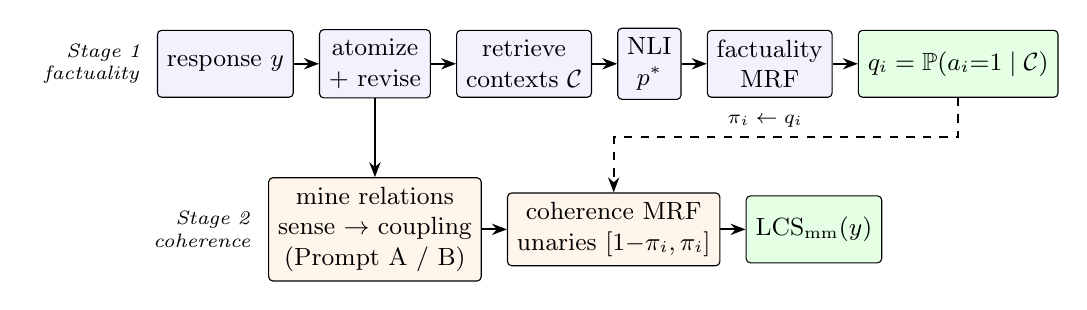
\begin{tikzpicture}[
    font=\small,
    box/.style={draw,rounded corners=1.5pt,align=center,inner sep=3.4pt,
                minimum height=8.5mm},
    s1/.style={box,fill=blue!5},
    s2/.style={box,fill=orange!8},
    fin/.style={box,fill=green!10},
    ar/.style={-{Stealth[length=1.9mm]},thick},
    node distance=3.2mm]

  \node[s1] (resp) {response $y$};
  \node[s1,right=of resp] (atom) {atomize\\+ revise};
  \node[s1,right=of atom] (ret)  {retrieve\\contexts $\mathcal{C}$};
  \node[s1,right=of ret]  (nli)  {NLI\\$p^\ast$};
  \node[s1,right=of nli]  (fmrf) {factuality\\MRF};
  \node[fin,right=of fmrf] (post) {$q_i=\pr{a_i{=}1\mid\mathcal{C}}$};

  \draw[ar] (resp) -- (atom);
  \draw[ar] (atom) -- (ret);
  \draw[ar] (ret)  -- (nli);
  \draw[ar] (nli)  -- (fmrf);
  \draw[ar] (fmrf) -- (post);

  % Mining emits the coupling, so there is no separate compile box.
  \node[s2,below=10mm of atom] (mine)
       {mine relations\\sense $\to$ coupling\\(Prompt A / B)};
  \node[s2,right=of mine] (cmrf)
       {coherence MRF\\unaries $[1{-}\pi_i,\pi_i]$};
  \node[fin,right=of cmrf] (lcs) {$\LCS_{\mm}(y)$};

  \draw[ar] (atom.south) -- ++(0,-4mm) -| (mine.north);
  \draw[ar] (mine) -- (cmrf);
  \draw[ar] (cmrf) -- (lcs);
  \draw[ar,dashed] (post.south) -- ++(0,-5mm) -| (cmrf.north)
        node[pos=0.28,above,font=\scriptsize]{$\pi_i \gets q_i$};

  \node[left=1mm of mine,font=\scriptsize\itshape,align=right,text width=13mm]
       {Stage 2\\coherence};
  \node[left=1mm of resp,font=\scriptsize\itshape,align=right,text width=13mm,
        yshift=0mm] {Stage 1\\factuality};
\end{tikzpicture}}
% scripts/make_pipeline_png.sh defines \plnocaption to render this figure for
% standalone export, where surrounding prose supplies the explanation. Undefined
% in the paper, so the caption below is typeset normally there.
\ifdefined\plnocaption\else
\caption{The two-stage pipeline. Stage 1 (\S\ref{sec-factuality}) is FactReasoner
  \citep{factreasoner}: it grounds each atom against retrieved evidence and returns a
  posterior marginal $q_i$. Stage 2 (\S\ref{sec-coherence}) builds a second MRF over
  the atoms \emph{alone} and adds one pairwise factor per mined atom--atom relation;
  the mined relation already carries its Level-1 coupling, so no separate compile step
  intervenes. The dashed arrow is the only coupling between the stages, and carries
  the composition $\pi_i\!\gets\!q_i$ into the $\phi_i=[1-\pi_i,\pi_i]$ of
  Def.~\ref{def-mrf}. Atomization is shared, so the response is decomposed once and
  both stages score the same claim set; setting $\pi_i\!\equiv\!\tfrac12$ instead
  recovers a pure coherence score that consults no external evidence
  (Rem.~\ref{rem-noevidence}).}
\label{fig:pipeline}
\fi
\end{figure}


\subsection{Decomposition, retrieval, and relation extraction}

A response $y$ is decomposed by an LLM \emph{atomizer} into atomic claims
$\mathcal{A}=\{a_1,\dots,a_n\}$, each a single independently verifiable proposition. A
\emph{reviser} then decontextualizes each one, resolving pronouns and anaphora so that the claim
is checkable outside its original sentence; near-duplicates are collapsed. For each claim a
retriever returns supporting passages, which are deduplicated into an evidence set
$\mathcal{C}=\{c_1,\dots,c_m\}$.

An LLM-based NLI extractor then labels admitted pairs. For a claim--evidence pair the label is
drawn from $\{\text{entailment},\text{contradiction},\text{neutral}\}$; for an evidence--evidence
pair both directions are scored and reconciled, with entailment in both directions relabelled
\emph{equivalence}. Neutral verdicts are dropped rather than encoded: a claim about which the
evidence is silent contributes no factor and is left at its prior, which is what makes the factor
set of \S\ref{sec-coherence} contain only the relations someone actually asserted.

\subsection{Reading a probability off the generation}
\label{sec-pstar}

Each retained relation carries a probability $p^\ast$. Rather than asking the model to verbalize a
confidence, we read it from the distribution over the tokens it actually emitted. The extractor is
prompted to end with a bracketed label; let $T$ be the set of generated tokens overlapping the
span of that label in the decoded text. Then
\begin{equation}
p^\ast \;=\; \exp\!\Big(\tfrac{1}{|T|}\textstyle\sum_{t\in T}\log p_t\Big),
\label{eq-pstar}
\end{equation}
the per-token geometric-mean probability of the label the model produced. Three details of this
construction are load-bearing, and we record them because each was a source of silent error.

\emph{Span alignment.} The probability is measured over exactly the span the label \emph{parser}
reports, reconstructing the decoded string from the token list and tracking each token's character
offsets. Measuring the same span the label came from makes the label and its probability
structurally unable to disagree. Requiring standalone bracket-delimiter tokens instead does not
work: tokenizers routinely fuse \texttt{[}, \texttt{]} and \texttt{"} into subwords with adjacent
characters, so a delimiter-based rule silently fails on some backends and not others.

\emph{Token-array conventions.} An earlier version of this code stripped the final entry of the
logprob array as an end-of-sequence token. OpenAI-compatible and vLLM logprob arrays contain only
emitted content tokens --- the stop is signalled out of band --- so dropping the last entry
deleted a real content token, and for a bracketed label that token is the one closing the label
whose confidence is being measured.

\emph{Degenerate cases.} When the logprob array is empty, no label span is found, or no token
aligns to it, the estimator returns $0.5$ rather than $0.0$. Returning zero would be read
downstream as a \emph{degenerate, impossible} relation for a label the model in fact generated,
which is a stronger claim than ``we could not measure the confidence''.

\emph{Backends without logprobs.} Some serving stacks expose no token logprobs at all. There
$p^\ast$ instead comes from SIMBA-UQ \citep{simbauq}, which samples the extractor repeatedly across
a temperature schedule, builds a pairwise similarity matrix over the samples, and aggregates each
sample's similarity row into a self-consistency confidence. The winning sample supplies the label
and its aggregated confidence supplies $p^\ast$, so the downstream model is unchanged.

\subsection{The factuality network and its variants}

The labelled graph becomes a pairwise MRF with one binary variable per claim and per evidence
passage. Unary factors are $\phi_X(x)=[1-\pi_X,\;\pi_X]$ with $\pi_X$ the prior on $X$; each
retained relation contributes one pairwise factor from Table~\ref{tab:factors} below, oriented so
the evidence passage is the premise. Marginals $\pr{A_i{=}1}$ are computed by weighted mini-bucket
elimination \citep{wmb} with i-bound $6$, and a claim is reported supported when
$\pr{A_i{=}1}>\tfrac12$.

Three graph variants differ in which factors are admitted: \textsc{fr1} connects each claim only
to the passages retrieved for it; \textsc{fr2} deduplicates passages and scores every claim
against all of them; \textsc{fr3} adds evidence--evidence factors. We use \textsc{fr2}. Because
scoring every claim against every passage is $O(nm)$ LLM calls, a candidate-pair policy can restrict
the pairs actually scored; the calibration of that policy is instructive for the analogous choice
in \S\ref{sec-mining}. Replaying policies against recorded verdicts on a 20-claim narrative with 60
passages, a provenance-restricted policy with an embedding similarity gate holds recall at $1.000$
through a threshold of $0.20$, slipping to $0.985$ at $0.30$ and $0.833$ at $0.40$. Substituting
token-Jaccard similarity for sentence embeddings, however, loses $22$ of $72$ non-neutral relations
and moves the factuality score by $0.05$ --- and \emph{no} threshold recovers full recall, even
$0.05$. Cheap surrogates for semantic similarity are not safe here, and the saving is
workload-dependent rather than constant: roughly $5\times$ on unrelated subtopics but $1.2\times$
on a narrative where every claim shares characters.

\paragraph{Conventions.} We use the with-priors factor tables (Table~\ref{tab:factors}) throughout,
with $\pi_C=0.9$ for evidence and $\pi_A=0.5$ for claims. The published factuality model uses the
no-priors tables and a higher evidence prior. The difference is immaterial to the coherence results
below, which set claim priors explicitly, but the convention must be stated because the two table
families are not interchangeable --- that is the subject of \S\ref{sec-potentials}.


%% ================================================================
\section{The relation taxonomy in full}
\label{app-taxonomy}
%% ================================================================

\S\ref{sec-levels} states the two-level taxonomy compactly. This appendix grounds every entry in a
realistic response excerpt, gives the compile map with its glosses and flags, and works one
coupling through by hand.

\subsection{One excerpt per inferential coupling}

\begin{table}[tp]
\centering\footnotesize
\setlength{\tabcolsep}{4pt}
\renewcommand{\arraystretch}{1.15}
\caption{One realistic response excerpt per Level-1 coupling of Def.~\ref{def-couplings}. As in
  Table~\ref{tab:senseex}, each excerpt is prose containing both claims --- \uline{$A$ is the
  source, underlined}, \textbf{$B$ the target, bold}, the \emph{italic} words drawing the link ---
  and $V(\tau)$ is repeated from Def.~\ref{def-couplings} so the excerpt can be read against the
  world it rules out. The \emph{Why} column names the world the response denies, which is what
  distinguishes each coupling from the one above it; the three conflict-adjacent couplings \con{},
  \exc{} and \cnc{} are illustrated on one two-part weld failure so that only exhaustiveness
  varies. \coupling{none} produces no factor, so its excerpt is one where the text relates the
  claims without constraining their truth.}
\label{tab:coupex}
\begin{tabularx}{\textwidth}{@{}l l l X@{}}
\toprule
Coupling & Reading & $V(\tau)$ & Response excerpt, and the world it denies \\
\midrule
\ent & $a_s\Rightarrow a_t$ & $\{(1,0)\}$
  & ``\uline{The alloy is chemically identical to the certified reference}, \emph{and therefore}
    \textbf{it meets the airframe specification}.''
    \newline\emph{Why:} the response rules out the world where the source holds and the target
    fails --- $(1,0)$ --- and says nothing about the case where the alloy differs, which is why
    the $a_s{=}0$ row returns the target to its prior. \\
\midrule
\con & $a_s\Rightarrow\neg a_t$ & $\{(1,1)\}$
  & ``\uline{The weld passed the tensile test}, \emph{yet} \textbf{the same joint was porous along
    its full length}.''
    \newline\emph{Why:} only the both-true world $(1,1)$ is denied. Both can still fail together
    --- if the wrong joint was tested, neither claim holds --- so $(0,0)$ must stay available. \\
\midrule
\exc & exactly one holds & $\{(0,0),(1,1)\}$
  & ``The joint was destructively examined, so \emph{exactly one of} \uline{the weld met the
    tensile minimum} \emph{and} \textbf{the weld fell short of it} \emph{must be the finding} ---
    \emph{there is no third outcome}.''
    \newline\emph{Why:} both same-value worlds are denied. The added $(0,0)$ is the whole
    difference from \con{}: once the joint has actually been examined the pair cannot both fail,
    so leaving that world open --- as \con{} does --- would under-penalize the conflict. \\
\midrule
\cnc & at least one holds & $\{(0,0)\}$
  & ``The fracture began at the joint, so \emph{at least one of} \uline{the weld} \emph{and}
    \textbf{the fastener} \emph{must have given way} --- conceivably both.''
    \newline\emph{Why:} the dual of \exc{}. Only the both-false world is denied, so asserting the
    disjunction is evidence \emph{for} both endpoints (Example~\ref{ex-cnc}). \\
\midrule
\eqv & $a_s\Leftrightarrow a_t$ & $\{(0,1),(1,0)\}$
  & ``\uline{The shipment was certified to specification} --- \emph{that is to say},
    \textbf{every contractual requirement had been met}.''
    \newline\emph{Why:} the two disagreeing worlds are denied, in both directions; unlike \ent{}
    there is no vacuous row, since a false source now also forces a false target. \\
\midrule
\coupling{none} & no coupling & $\varnothing$
  & ``\uline{The replacement units were installed in March}, \emph{some three months before}
    \textbf{the first in-flight failures were reported}.''
    \newline\emph{Why:} no world is denied. The response genuinely relates the claims, but
    ordering them in time constrains neither one's truth, so the pair contributes
    \textbf{no factor} and both claims stay at their priors. \\
\bottomrule
\end{tabularx}
\end{table}

Table~\ref{tab:coupex} gives a response excerpt for each coupling, set against the world that
coupling denies; since a coupling \emph{is} its penalized set, reading the two together is the
quickest way to see what each one commits the response to. The first three couplings are exactly
the NLI edge types of \S\ref{app-stage1}, which is what lets a mined relation reuse the
existing graph machinery unchanged. The last two are additions required by argumentative prose,
and the distinction between them and \con{} is the one the taxonomy exists to draw.

\paragraph{Why exhaustiveness needs its own coupling.} \con{} forbids only the both-true world: two
claims that cannot both hold, but might both fail. \exc{} additionally forbids the both-false
world, which is what \emph{exhaustive} alternatives assert. ``No one was harmed'' and ``three
people died'' can neither both hold nor both fail --- either someone was harmed or no one was ---
so a model that treats them as mere opposition has mis-described the situation in a way that
matters for scoring: it leaves available a world in which \emph{neither} claim is true, and so
under-penalizes. Conversely \cnc{} is the dual, penalizing only the both-false world, and is what a
disjunction asserts (``at least one of these two findings must hold''). Adjudicated disputes ---
incident investigations, litigation, competing hypotheses --- are precisely the domains where
exhaustive pairs occur, because the function of a finding is to close one. The \con{}, \exc{} and
\cnc{} rows of Table~\ref{tab:coupex} state one two-part weld failure three times over, so that
the only thing varying across them is which same-value worlds the response leaves standing.

\begin{example}[A \cnc{} factor in isolation]
\label{ex-cnc}
Take a single \cnc{} relation with $p=0.9$ over two claims with priors $\pi=0.5$, and no other
factors. From Table~\ref{tab:factors} the pairwise table is $[1-p,\;\pi_s,\;\pi_s,\;p]
=[0.1,0.5,0.5,0.9]$, and multiplying in the unaries and normalizing gives world masses
\[
\pr{0,0}=0.05,\quad \pr{0,1}=0.25,\quad \pr{1,0}=0.25,\quad \pr{1,1}=0.45 .
\]
The both-false world is suppressed from the $0.25$ it would receive under independent fair priors
to $0.05$, while the three worlds satisfying ``at least one holds'' share the recovered mass in
proportion to how many endpoints they assert. Each marginal rises from $0.5$ to $0.7$: asserting
that at least one of two claims holds is evidence for both, which is the intended reading.
\end{example}


\subsection{The compile map, with glosses}

\begin{table}[tbp]
\centering\small
\caption{The compile map $\mathcal{C}$ of \S\ref{sec-levels}, with glosses. \emph{Ordering-only} senses
  record assertion order but induce \textbf{no factor}, which is what makes an order-only edit
  provably score-invariant (Rem.~\ref{rem-order}). \sense{Concession} is a conflict the text may
  itself resolve, handled by Eq.~\ref{eq-concession}. The nine senses marked $\star$ form the
  admissible vocabulary of \S\ref{sec-mining}.}
\label{tab:compile}
\begin{tabular}{@{}llccll@{}}
\toprule
Level-2 sense & $\mathcal{C}$ coupling & prior & dir. & flag & gloss \\
\midrule
\sense{Cause-Effect}$^\star$   & \ent & $\bot$ & yes & & source brings target about \\
\sense{Effect-Cause}$^\star$   & \ent & $\bot$ & yes & & source is the effect, target the cause \\
\sense{Evidence}$^\star$       & \ent & $\bot$ & yes & & source is evidence for target \\
\sense{Condition}              & \ent & $\bot$ & yes & & source conditions target \\
\sense{Instantiation}          & \ent & $\bot$ & yes & & target instantiates source \\
\sense{Restatement}$^\star$    & \eqv & $0.90$ & no  & & definitional identity \\
\sense{Contrast}$^\star$       & \con & $\bot$ & no  & & opposed, \emph{not} exhaustive \\
\sense{Concession}$^\star$     & \con & $\bot$ & yes & conc. & a tension the text resolves \\
\sense{Alternative}$^\star$    & \exc & $\bot$ & no  & & exhaustive: exactly one holds \\
\sense{Disjunction}$^\star$    & \cnc & $\bot$ & no  & & at least one holds \\
\sense{Precedence}$^\star$     & \coupling{none} & --- & yes & ord. & temporal order only \\
\sense{Succession}             & \coupling{none} & --- & yes & ord. & temporal order only \\
\bottomrule
\end{tabular}
\end{table}

Couplings are the right vocabulary for a factor table and the wrong one for annotation. Asked
whether two claims stand in \ent{}, an annotator --- human or model --- has been handed a question
about logic, when the fact actually observable in the text is a question about discourse: does this
sentence give a cause, offer evidence, concede a tension, or lay out alternatives? We therefore
mine an interpretable layer and compile it down.


\subsection{One excerpt per discourse sense}

\begin{table}[tp]
\centering\footnotesize
\setlength{\tabcolsep}{4pt}
\renewcommand{\arraystretch}{1.15}
\caption{One realistic response excerpt per Level-2 sense of Table~\ref{tab:compile}, in the same
  row order and grouped by the coupling each compiles to. Each excerpt is prose of the kind the
  estimator actually sees and \emph{contains both claims}: \uline{$A$ is underlined}, \textbf{$B$ is
  bold}, and the \emph{italic} words are the ones that draw the link --- the span
  \S\ref{sec-mining} obliges the model to quote, which is why it must be findable in the response
  and not in either claim. Senses are marked $\star$ when admissible; the three unmarked ones are
  included because their breadth is the argument for excluding them (\S\ref{sec-mining}). The
  \sense{Contrast}, \sense{Alternative} and \sense{Disjunction} rows describe one two-part weld
  failure three ways, separated only by exhaustiveness (\S\ref{sec-levels}); they reuse the
  scenario of Table~\ref{tab:coupex} deliberately, so that a discourse sense and the coupling it
  compiles to can be compared on the same prose.}
\label{tab:senseex}
\begin{tabularx}{\textwidth}{@{}llX@{}}
\toprule
Level-2 sense & $\mathcal{C}$ & Response excerpt, and why this sense rather than a neighbour \\
\midrule
\sense{Cause-Effect}$^\star$ & \ent
  & ``\uline{The company shipped a batch it knew to be out of tolerance}, and \emph{as a direct
    result} \textbf{its share price fell $15\%$ that quarter}.''
    \newline\emph{Why:} the response itself presents $A$ as bringing $B$ about; the marker names the
    direction. \\
\sense{Effect-Cause}$^\star$ & \ent
  & ``\uline{The entire fleet was grounded on 14 March}. The order came \emph{because}
    \textbf{inspectors had found a cracked wing spar on two airframes}.''
    \newline\emph{Why:} the same support runs from the stated effect to its cause. Direction of
    \emph{explanation} is reversed; direction of inferential support is not. \\
\sense{Evidence}$^\star$ & \ent
  & ``\uline{The maintenance log records no inspection between January and June}, \emph{which
    shows that} \textbf{the mandatory 500-hour check was skipped}.''
    \newline\emph{Why:} $A$ is offered in support of $B$ without any claim that it caused it ---
    a record is evidence, not a mechanism. \\
\sense{Condition} & \ent
  & ``\textbf{A part is cleared for airframe use} \emph{only if} \uline{its alloy meets the
    reference specification}.''
    \newline\emph{Why:} $B$ is asserted contingent on $A$. Note how weakly the cue constrains:
    nearly any dependence can be reread as a condition, which is why the sense is inadmissible. \\
\sense{Instantiation} & \ent
  & ``\uline{Several suppliers failed the 2023 audit} --- \emph{for instance},
    \textbf{the Tucson plant failed on two counts}.''
    \newline\emph{Why:} $B$ is one case falling under $A$'s generalization. Like
    \sense{Condition}, broad enough to fit almost any pair that shares a topic. \\
\midrule
\sense{Restatement}$^\star$ & \eqv
  & ``\uline{The shipment was certified to specification} --- \emph{in other words},
    \textbf{every requirement in the contract had been met}.''
    \newline\emph{Why:} a \emph{marked} paraphrase asserts identity of content, which is why the
    strength prior is fixed at $0.90$ rather than estimated. \\
\midrule
\sense{Contrast}$^\star$ & \con
  & ``\uline{The weld passed the tensile test}, \emph{but} \textbf{the same joint was porous
    along its full length}.''
    \newline\emph{Why:} opposed and \emph{not} exhaustive. A third possibility --- the wrong joint
    was tested --- leaves both false, so the both-false world must stay available. \\
\sense{Concession}$^\star$ & \con
  & ``\emph{Although} \uline{the airline argued throughout that pilot error was to blame},
    \textbf{the final report identified a metallurgical defect}; the tribunal \emph{ultimately
    held} for the latter.''
    \newline\emph{Why:} a tension the text itself settles. The resolving holding triggers the
    discount of Eq.~\ref{eq-concession} rather than counting as a live conflict. \\
\midrule
\sense{Alternative}$^\star$ & \exc
  & ``The two accounts cannot be reconciled: \emph{either} \uline{no one aboard was harmed},
    \emph{or} \textbf{three passengers died}, and \emph{exactly one of them is true}.''
    \newline\emph{Why:} exhaustive. Unlike \sense{Contrast} the pair can neither both hold nor
    both fail, so the both-false world is penalized too. \\
\midrule
\sense{Disjunction}$^\star$ & \cnc
  & ``Metallurgy confirms the fracture began at the joint, so \emph{at least one of}
    \uline{the weld} \emph{and} \textbf{the fastener} \emph{must have failed} --- possibly
    both.''
    \newline\emph{Why:} at least one holds and both may. The dual of \sense{Alternative}:
    only the both-false world is penalized. \\
\midrule
\sense{Precedence}$^\star$ & \coupling{none}
  & ``\uline{The replacement units were installed in March}, \emph{some three months before}
    \textbf{the first in-flight failures were reported in June}.''
    \newline\emph{Why:} the text genuinely relates the two claims, and says nothing about either
    one's truth --- so the sense induces \textbf{no factor}. \\
\sense{Succession} & \coupling{none}
  & ``\textbf{The first in-flight failures were reported in June}, \emph{fully three months
    after} \uline{the replacement units had been installed}.''
    \newline\emph{Why:} the mirror of \sense{Precedence} --- the same two claims, the same
    absence of truth-functional content. Offering both senses invites an arbitrary choice on a
    relation that produces no factor either way. \\
\bottomrule
\end{tabularx}
\end{table}

Table~\ref{tab:senseex} grounds each sense in a response excerpt that contains both claims and
the wording that licenses the link, since what an annotator must actually recognize is a form of
words rather than a truth-functional pattern. Several entries encode judgements worth defending. \sense{Restatement}
carries a fixed strength prior of $0.90$ because a marked paraphrase (``in other words'',
``equivalently'') is a claim about identity of content, and a model asked to estimate its strength
has little to add; the estimator's value is used when available, and the prior seeds it otherwise.
Five senses collapse onto \ent{}, which is a deliberate loss: the model does not distinguish
causation from evidence, because a pairwise potential over truth values cannot. The grouped \ent{}
block of Table~\ref{tab:senseex} shows exactly what compilation discards --- five distinct
discourse facts, one factor table. What survives compilation is the inferential force, and the
sense is retained alongside it for interpretability and for error analysis.

The \sense{Contrast}/\sense{Alternative} boundary is exactly the exhaustiveness question of
\S\ref{sec-levels}, and the \sense{Contrast}, \sense{Alternative} and \sense{Disjunction} rows of
Table~\ref{tab:senseex} are that question in concrete form: one two-part weld failure written up
three ways --- as mere opposition, as an exhaustive choice, and as a disjunction --- differing in
nothing but which same-value worlds the response leaves available. The two
ordering-only senses are the taxonomy's way of representing a
relation the text genuinely draws while asserting that it has no truth-functional content: a
narrative that says one event preceded another has related the two claims, and has said nothing
about whether either is true.


%% ================================================================
\section{Potentials and the four coherence readouts}
\label{app-readouts}
%% ================================================================

\subsection{Both families of pairwise potentials}

\begin{table}[tbp]
\centering\small
\caption{Pairwise potentials $\psi_{\tau,p}(a_s,a_t)$, listed row-major over the assignments
  $(0,0),(0,1),(1,0),(1,1)$; $\pi_s$ is the source claim's prior and bold marks the penalized set
  $V(\tau)$ of Def.~\ref{def-couplings}. The \emph{no-priors} family is correct for
  claim--evidence factuality, where the source passage's own truth is at stake; the
  \emph{with-priors} family is what coherence requires (Prop.~\ref{prop-rowstoch}) and what
  Def.~\ref{def-mrf} uses. The two symmetric couplings \eqv{} and \exc{} coincide in both
  families, having no source-prior term to correct.}
\label{tab:factors}
\begin{tabular}{@{}llll@{}}
\toprule
Coupling $\tau$ & No priors & With priors & Symmetry \\
\midrule
\ent  & $[p,\;p,\;\mathbf{1\!-\!p},\;p]$
      & $[1\!-\!\pi_s,\;\pi_s,\;\mathbf{1\!-\!p},\;p]$ & asymmetric \\
\con  & $[p,\;p,\;p,\;\mathbf{1\!-\!p}]$
      & $[1\!-\!\pi_s,\;\pi_s,\;p,\;\mathbf{1\!-\!p}]$ & asymmetric \\
\eqv  & \multicolumn{2}{l}{$[p,\;\mathbf{1\!-\!p},\;\mathbf{1\!-\!p},\;p]$} & symmetric \\
\exc  & \multicolumn{2}{l}{$[\mathbf{1\!-\!p},\;p,\;p,\;\mathbf{1\!-\!p}]$} & symmetric \\
\cnc  & $[\mathbf{1\!-\!p},\;p,\;p,\;p]$
      & $[\mathbf{1\!-\!p},\;\pi_s,\;\pi_s,\;p]$ & symmetric \\
\bottomrule
\end{tabular}
\end{table}


\S\ref{sec-potentials} states Prop.~\ref{prop-rowstoch} and the collapse it prevents. The table
above gives both families side by side: the \emph{no-priors} family is correct for claim--evidence
factuality, where the source passage's own truth is at stake, and the \emph{with-priors} family is
what coherence requires. The two symmetric couplings \eqv{} and \exc{} coincide in both families,
having no source-prior term to correct.

\subsection{The four readouts}

Definition~\ref{def-mrf} specifies a distribution; a coherence score is a functional of it, and
several are defensible. We state five criteria, define four candidates with their exact
constructions, and then decide between them by exact inference rather than by preference.

\begin{definition}[Criteria]
\label{def-criteria}
A coherence readout should be:
\textbf{(R1)} a genuine functional of the joint $\pr{\mathbf{a}}$, not of the relation list alone;
\textbf{(R2)} valued in $[0,1]$ and interpretable;
\textbf{(R3)} \emph{monotone} --- resolving or removing a conflict must not decrease it;
\textbf{(R4)} sensitive to conflict without hand-tuned constants;
\textbf{(R5)} computable from standard inference queries.
\end{definition}

R1 deserves comment, since it is the criterion that does the most work. A readout that depends only
on $\mathcal{R}$ --- how many relations there are, what types, what weights --- is not measuring the
response; it is measuring its own annotation. Proposition~\ref{prop-vacuous} below shows this is not
a hypothetical concern.

\subsection{(a) Mean posterior marginal}

\begin{equation}
\LCS_{\mm}(y) \;=\; \frac{1}{n}\sum_{i=1}^{n}\pr{a_i=1} .
\label{eq-mm}
\end{equation}

The marginals come directly from a single \textsc{mar} query. The interpretation is the expected
fraction of the response's claims that the argument, taken as a whole, upholds. A conflict
suppresses the marginals of its endpoints; a satisfied entailment chain propagates support along
itself; a claim no relation touches stays at its prior and contributes neutrally.

Alongside the scalar we report three diagnostics that come free with the same query: the per-claim
marginals themselves, which localize an incoherence to specific claims; the count of claims dragged
\emph{below their own prior}, which is the sharpest single indicator of an active conflict; and the
mean normalized binary entropy $\mathcal{E}=\tfrac1n\sum_i H_2(q_i)$, lower being more decisive.

\subsection{(b) Consistency: a two-term probability}
\label{sec-consistency}

The obvious alternative to averaging marginals is to ask for the probability that the response is
consistent. Making that precise turns out to require two terms:
\begin{equation}
\LCS_{\cons} = \tfrac12\bigl(\mathcal{K}+\mathcal{S}\bigr),\quad
\mathcal{K} = \pr{\!\!\bigwedge_{r:\,\tau_r=\con}\!\!\neg\bigl(a_{s_r}\!\wedge a_{t_r}\bigr)},\quad
\mathcal{S} = \frac{\sum_{r\in\mathcal{R}_{\mathcal{S}}} p_r\,U_r}
                   {\sum_{r\in\mathcal{R}_{\mathcal{S}}} p_r},
\label{eq-cons}
\end{equation}
where $\mathcal{R}_{\mathcal{S}}$ ranges over $\{\ent,\eqv,\exc\}$ and $U_r$ is the probability that
relation $r$ is \emph{actively upheld}:
\[
U_r=\pr{a_{s_r}{=}1 \wedge a_{t_r}{=}1}\ \text{ for }\ent,\eqv,
\qquad
U_r=\pr{a_{s_r}\neq a_{t_r}}\ \text{ for }\exc .
\]

\paragraph{The two coupling sets are deliberately different.} The conflict event $\mathcal{K}$ keys
on \con{} alone, even though $\mathcal{T}_{\mathrm{conf}}=\{\con,\exc\}$. The reason is that an
\exc{} spreads its incoherence over \emph{both} same-value worlds, so reading only its both-true half
would describe half the coupling and silently report the other half as satisfactory. \exc{} therefore
earns credit in $\mathcal{S}$ instead, where its exactly-one world is simultaneously where the
exclusion is honoured and where it is informative. \cnc{} enters neither term: its defect is the
both-false world, which (a)'s marginals already see directly.

\paragraph{Computing $\mathcal{K}$ exactly.} $\mathcal{K}$ is an event probability over a conjunction
of $|\{r:\tau_r=\con\}|$ pairwise events, which a naive encoding would represent as a factor of
exponential arity. Instead we augment the network with deterministic auxiliary variables: one
$u_r$ per conflict edge with a ternary factor enforcing $u_r = a_{s_r}\wedge a_{t_r}$, then a chained
running disjunction $U_k = U_{k-1}\vee u_k$ with ternary factors, and finally
$\mathcal{K}=\pr{U_{|\cdot|}{=}0}$. Every auxiliary factor is deterministic and at most ternary, so
no $2^{|\mathcal{R}|}$ table is ever built and the augmented network is read with one \textsc{mar}.

\paragraph{Computing $\mathcal{S}$ exactly.} $\mathcal{S}$ is not an event probability but a weighted
sum of \emph{pairwise joints} --- a linear functional of the joint --- so it cannot be read off the
same accumulator chain. It needs one deterministic indicator variable per supported edge and its own
\textsc{mar}. Because the indicators are mutually independent given the base network, they may be
batched across several queries without approximation, which matters only for inference backends that
enumerate.

\paragraph{Why ``actively upheld'' and not ``satisfied''.} The definition of $U_r$ credits a relation
only in the informative world, not in every world where it is technically satisfied. An entailment
$a_s\Rightarrow a_t$ is satisfied vacuously whenever $a_s=0$, and crediting that is fatal:

\begin{proposition}[The vacuous-truth trap]
\label{prop-vacuous}
Let $\mathcal{K}'=\pr{\text{every relation in }\mathcal{R}\text{ is satisfied}}$, the apparently
natural extension of $\mathcal{K}$ to all couplings. Then a response with no mined relations
satisfies $\mathcal{K}'=1$, the maximum attainable value.
\end{proposition}

\begin{proof}
$\mathcal{K}'$ is the probability of an intersection of $|\mathcal{R}|$ events; for
$\mathcal{R}=\varnothing$ the intersection is the whole space.
\end{proof}

The proposition is immediate, but its consequence is not, and it is the reason
$\LCS_{\cons}$ has the form it does. Measured on the family of \S\ref{sec-example-aero}, a disconnected
bag of claims scores $\mathcal{K}'=1.000$ while a response whose causal spine is fully satisfied
scores $0.221$ --- an inversion, not a tie. Nor is the defect repaired by count normalization: the
geometric mean over relations gives $0.883$ for the base response against $0.882$ for the coherent
one, non-monotone \emph{and} still $1.000$ on the bag; the expected fraction of satisfied relations
gives $0.857$ against $0.852$, likewise inverted; and normalizing against a prior ceiling leaves
$[0,1]$ altogether ($8.82$ against $5.46$) while still running backwards. The common cause is that
``are the asserted relations honoured?'' is a property of $\mathcal{R}$ rather than of $y$ --- a
violation of R1 --- and it is maximized by asserting nothing. Crediting only the informative world
removes the free lunch: a bag of claims upholds nothing and scores $\mathcal{S}=0$.

The two terms are averaged rather than multiplied so that neither can annihilate the other. A live
contradiction should not erase a well-supported spine, and a relation-free response should not
inherit a perfect score from an empty conflict set.

\subsection{(c) A reified coherence node}
\label{sec-reified}

The most direct reading of ``is this response coherent?'' as a single probability is to introduce a
variable for it. Add a binary $R$ with Bernoulli prior $\rho$ and, for each relation, a ternary
\emph{vote} factor
\begin{equation}
h_r(R,a_s,a_t)=\begin{cases}
1 & R=0 \quad\text{(the branch is flat)}\\
1 & R=1,\ (a_s,a_t)\notin V(\tau_r)\\
1-p_r & R=1,\ (a_s,a_t)\in V(\tau_r),
\end{cases}
\qquad \LCS_{\rei}=\pr{R=1}.
\label{eq-reified}
\end{equation}
In the $R=1$ branch each violated relation charges $1-p_r$, so $R$ behaves as a noisy-AND over
relation satisfaction; in the $R=0$ branch nothing is charged, so $R=0$ carries no commitment. With
no relations $R$ is decoupled and $\LCS_{\rei}=\rho$, correctly signalling that nothing was measured.
Note that the violated set is $V(\tau)$ from Def.~\ref{def-couplings}, so \ent{} is treated as
satisfied at $a_s=0$ --- vacuously --- which is where (c) inherits a weaker form of
Prop.~\ref{prop-vacuous}'s problem. Appendix~\ref{app-reified} works a three-claim subnet through by
hand, giving $\pr{R{=}1}=0.453$.

\subsection{(d) Normalized log-partition}
\label{sec-logz}

The partition function measures how much probability mass the constraints leave standing, which is a
global coherence signal requiring no marginals at all. It is unnormalized, so we grade it between two
references built from the same edge skeleton:
\begin{equation}
\LCS_{\lp} \;=\; \frac{\log Z - \log Z_{\min}}{\log Z_{\max} - \log Z_{\min}} .
\label{eq-logz}
\end{equation}
For the ceiling, $Z_{\max}$ is the partition function of the same network with every conflict edge
removed: deleting constraint factors only adds mass, so $\log Z\le\log Z_{\max}$ always. For the
floor we take the \emph{MAP world mass} of the base network,
$Z_{\min}=\max_{\mathbf{a}}\prod_i\phi_i\prod_r\psi_r$.

\begin{lemma}[The MAP world mass is a valid, coherence-graded floor]
\label{lem-floor}
$\log Z_{\min}\le\log Z$ for every network, and $Z_{\min}$ is non-increasing in conflict strength.
\end{lemma}
\begin{proof}
$Z=\sum_{\mathbf{a}}\mathrm{mass}(\mathbf{a})$ is a sum of non-negative terms, so its single largest
term is a lower bound. For the second claim, increasing $p_r$ on a conflict edge multiplies the mass
of every world in $V(\tau_r)$ by a factor below one and leaves other worlds unchanged, so the maximum
over worlds cannot increase.
\end{proof}

Lemma~\ref{lem-floor} is not a technicality; it replaces two floors that look more natural and are
wrong. Retyping every edge to \con{}, or saturating conflicts to $p=1$, both fail to bound $\log Z$
below for the row-stochastic tables of Prop.~\ref{prop-rowstoch}: an isolated conflict removes no
mass at all when its endpoints sit at the uniform prior --- the setting in which both candidates were
checked --- and little away from it, whereas a mass-concentrating entailment backbone concentrates a
great deal, so a network combining a strong backbone with several soft conflicts can have a base
$\log Z$ \emph{below} either candidate floor. We observed exactly this on real graphs, which put
Eq.~\ref{eq-logz} outside $[0,1]$ until the MAP floor replaced them. In practice we clamp the ratio
to $[0,1]$ regardless, since approximate inference computes $\log Z$ and the MAP bound with finite
i-bound and small tolerance violations are possible.

\subsection{Deciding between the four}
\label{sec-selection}

\begin{table}[tbp]
\centering\small
\caption{All four readouts across a coherence-ordered family of five variants of one response, by
  exact inference over $2^{16}$ worlds. The variants run from least to most coherent left to right in
  the intended ordering. Bold marks a value that moves the \emph{wrong} way relative to its
  predecessor. Only (a) and (d) are monotone throughout.}
\label{tab:allcands}
\begin{tabular}{@{}lccccc@{}}
\toprule
Variant & (a) $\LCS_{\mm}$ & (b) $\LCS_{\cons}$ & (c) $\LCS_{\rei}$ & $\log Z$ & (d) $\LCS_{\lp}$ \\
\midrule
\emph{worse}       & $0.586$ & $\mathbf{0.778}$ & $0.116$ & $-10.54$ & $0.68$ \\
\emph{base}        & $0.607$ & $0.781$          & $0.148$ & $-9.64$  & $0.78$ \\
\emph{concession}  & $0.612$ & $\mathbf{0.772}$ & $\mathbf{0.134}$ & $-9.64$ & $0.80$ \\
\emph{fixcasualty} & $0.613$ & $\mathbf{0.764}$ & $0.156$ & $-8.95$  & $0.89$ \\
\emph{coherent}    & $0.620$ & $\mathbf{0.752}$ & $0.181$ & $-8.25$  & $1.00$ \\
\midrule
\textbf{monotone?} & \textbf{yes} & no & no & \textbf{yes} & \textbf{yes} \\
\bottomrule
\end{tabular}
\end{table}

\begin{table}[tbp]
\centering\small
\caption{The four readouts against the criteria of Def.~\ref{def-criteria}, with the inference
  queries each requires.}
\label{tab:criteria}
\begin{tabular}{@{}llccccc l@{}}
\toprule
Readout & Queries & R1 & R2 & R3 & R4 & R5 & Note \\
\midrule
(a) mean marginal   & \textsc{mar} & \checkmark & \checkmark & \checkmark & \checkmark & \checkmark & \textbf{selected} \\
(b) consistency     & \textsc{mar}$\times2$ & \checkmark & \checkmark & $\times$ & \checkmark & \checkmark & concession dip \\
(c) reified         & \textsc{mar} & \checkmark & \checkmark & $\times$ & $\times$ & \checkmark & free $\rho$; dip \\
(d) norm.\ $\log Z$ & \textsc{pr}, \textsc{map} & \checkmark & \checkmark & \checkmark & \checkmark & \checkmark & needs 2 references \\
\bottomrule
\end{tabular}
\end{table}

Table~\ref{tab:allcands} settles the question empirically and Table~\ref{tab:criteria} summarizes.
Readouts (b) and (c) both fail R3, and they fail it at the \emph{same} variant --- the one where a
conceded tension is resolved --- for a shared reason that is worth stating precisely, because it
looks like an implementation bug and is not.

\begin{proposition}[Belief versus event activity]
\label{prop-quirk}
Softening a resolved conflict via Eq.~\ref{eq-concession} \emph{increases} the probability of its
both-true world. For a single conflict edge with uniform priors, discounting $p$ from $0.80$ to
$0.55$ moves $\pr{a_s{=}1,a_t{=}1}$ from $0.10$ to $0.225$.
\end{proposition}
\begin{proof}
Under both conflict couplings the $(1,1)$ cell of Table~\ref{tab:factors} is $1-p$, which increases as
$p$ falls. Take a lone \con{} edge with $\pi_s=\pi_t=\tfrac12$, so the with-priors table is
$[\tfrac12,\tfrac12,p,1-p]$ and each world carries an equal unary factor of $\tfrac14$. The
unnormalized masses are then proportional to the table itself, giving
$\pr{1,1}=(1-p)/\bigl(\tfrac12+\tfrac12+p+(1-p)\bigr)=(1-p)/2$, which is monotone decreasing in $p$.
Evaluating at $p=0.80$ and $p=0.55$ gives $0.100$ and $0.225$.
\end{proof}

The consequence sorts the four readouts into two kinds. A readout that asks \emph{is the conflict
active} --- (b) counts exactly that event, (c) charges $1-p_r$ for it --- must register a softened
conflict as \emph{more} often active, and therefore dips. A readout that asks \emph{how strongly
should each claim be believed} --- (a) through marginals, (d) through mass --- sees less suppression
and rises. Since resolving a concession is by construction an increase in coherence, a coherence
score must track belief rather than event activity. That is the substantive finding of this section,
and it is not specific to our parameterization: any readout defined as the probability of a
conflict-free configuration will invert under any discount-based treatment of resolved concessions.

\paragraph{A second failure mode of (b).} Table~\ref{tab:allcands} shows (b) failing worse than a
single dip, and the reason is instructive about $\mathcal{K}$ and $\mathcal{S}$ jointly. In this
family both conflicts are \exc{} rather than \con{}, so $\mathcal{K}\equiv1.000$ throughout by the
coupling-set decision above, and the score is carried entirely by $\mathcal{S}$. But removing an
exclusion removes \emph{support} credit as well as conflict, so the score runs backwards from
$0.778$ to $0.752$ across the whole ladder. On three-coupling variants of the same response, where
the conflicts are \con{} and $\mathcal{K}$ is live, (b) instead runs
$0.576 \to 0.654 \to \mathbf{0.582} \to 0.672 \to 0.752$: correctly ordered apart from the concession
dip. Either way it is non-monotone, and the lesson is that $\mathcal{K}$ and $\mathcal{S}$ should be
read separately as diagnostics rather than averaged into a headline.

\paragraph{Selection.} We report (a) as the headline. It satisfies all five criteria, needs a single
\textsc{mar} query, and is the only one of the four whose value decomposes into per-claim
contributions --- which is what makes an incoherence \emph{locatable} rather than merely detectable.
We compute and report all four, since (d) is a genuine alternative satisfying the same criteria
through a different route (mass rather than marginals), and $\mathcal{K}$, $\mathcal{S}$ carry
diagnostic information the mean marginal does not expose.

\subsection{Algorithm and cost}
\label{sec-algo}

\begin{algorithm}[t]
\caption{\textsc{ComputeLCS}$(y)$ --- the end-to-end coherence score.}
\label{alg-lcs}
\begin{algorithmic}[1]
\Require response $y$; relation estimator $\mathcal{M}$; discount $\lambda$; priors $\pi$
\Ensure $\LCS\in[0,1]$, marginals $\{q_i\}$, diagnostics
\State $\mathcal{A} \gets \textsc{AtomizeAndDecontextualize}(y)$
\State $P \gets \textsc{SelectCandidatePairs}(\mathcal{A}, y, \dots)$ \Comment{Algorithm~\ref{alg-pairs}}
\State $\mathcal{R} \gets \varnothing$
\ForAll{$(a_i,a_j) \in P$} \Comment{concurrent, rate-limited}
  \State $(\text{sense}, \tau, c) \gets \textsc{PromptA}(a_i,a_j,y)$ \Comment{$c=\pr{\tau\mid\cdot}$ from Eq.~\ref{eq-pstar}}
  \If{$\tau = \coupling{none}$} \textbf{continue} \EndIf
  \State $\sigma \gets \textsc{PromptB}(a_i,a_j,\tau,y)$ \Comment{surrogate-token strength}
  \State $\mathcal{R} \gets \mathcal{R} \cup \{(i,j,\tau,\ \mathrm{clip}_{[0,1]}(c\cdot\sigma))\}$
\EndFor
\ForAll{$r \in \mathcal{R}$ with $\tau_r\in\mathcal{T}_{\mathrm{conf}}$ sensed as \sense{Concession}}
  \If{a resolving holding $h$ exists} $p_r \gets p_r(1-\lambda\pi_h)$
  \Else{} mark $r$ unresolved \EndIf
\EndFor
\State $\mathcal{N} \gets$ network of Eq.~\ref{eq-joint} over $(\mathcal{A},\mathcal{R},\pi)$
  \Comment{with-priors tables}
\State $\{q_i\} \gets \textsc{Infer}(\mathcal{N}, \textsc{mar})$
\State \Return $\tfrac1n\sum_i q_i$, $\{q_i\}$, $\bigl(\#\{q_i<\pi_i\},\ \mathcal{E},\ \log Z\bigr)$
\end{algorithmic}
\end{algorithm}

Algorithm~\ref{alg-lcs} is dominated by steps 4--9: $|P|$ Prompt-A calls plus one Prompt-B call per
surviving edge, which the candidate policy keeps near-linear in $n$ rather than quadratic. Inference
is negligible by comparison.

Answering all four readouts requires seven inference calls: the base \textsc{mar} and \textsc{pr},
the $\mathcal{K}$ accumulator \textsc{mar}, the $\mathcal{S}$ indicator \textsc{mar}, the reified
\textsc{mar}, the conflict-free ceiling \textsc{pr}, and the base \textsc{map}. Computed
independently they would cost fourteen, since each readout re-runs the shared base pair. Production
inference is weighted mini-bucket \citep{wmb} with i-bound $6$; every \emph{exact} value reported in
this paper instead comes from explicit $2^n$ enumeration, which we use as a regression oracle for
$n\le20$ and which is the source of Tables~\ref{tab:allcands} and the values in
\S\ref{app-examples}.


%% ================================================================
\section{Relation mining in detail}
\label{app-mining}
%% ================================================================

\subsection{Candidate-pair selection}

\begin{algorithm}[t]
\caption{\textsc{SelectCandidatePairs}: response-anchored candidate selection.}
\label{alg-pairs}
\begin{algorithmic}[1]
\Require claims $\mathcal{A}=\langle a_1,\dots,a_n\rangle$ in assertion order; response $y$;
  policy; window $w$; gate threshold $\theta_g$; discourse thresholds $\theta_d,\delta$
\Ensure ordered candidate pairs $P$, plus a coverage record
\If{policy $=$ \textsc{all\_pairs}} \Return every ordered pair $(a_i,a_j)$, $i\neq j$ \EndIf
\State $W \gets \{(a_i,a_j) : 0 < j-i \le w\}$ \Comment{forward order window}
\If{policy $=$ \textsc{bidirectional}} $W \gets W \cup \{(a_j,a_i) : 0 < j-i \le w\}$ \EndIf
\State $G \gets \varnothing$
\If{policy $=$ \textsc{gated}}
  \State $G \gets \{(a_i,a_j) : j-i > w,\ \mathrm{sim}(a_i,a_j)\ge\theta_g\}$
\EndIf
\State align each claim to its best-matching sentence of $y$
\State $\mathit{Prom} \gets \{(a_i,a_j)\notin W\cup G : \textsc{DiscourseAdjacent}(i,j)\}$
\State $\mathit{Dem} \gets \{(a_i,a_j)\in W : \neg\,\textsc{DiscourseAdjacent}(i,j)\}$
\State \Return $\bigl(\textsc{Dedup}(W \cup G \cup \mathit{Prom}) \setminus \mathit{Dem}\bigr)$,
  $\;(|W|,|G|,|\mathit{Prom}|,|\mathit{Dem}|)$
\end{algorithmic}
\end{algorithm}


Each claim is aligned to its originating sentence; a pair is \emph{discourse-adjacent} if the two
claims share content tokens above a Jaccard threshold, if their sentences are within a short span,
or if the target's sentence opens with a discourse connective. Out-of-window pairs that are
discourse-adjacent are \emph{promoted} into the candidate set; in-window pairs that are not are
\emph{demoted} out of it. The refinement is a correlated filter --- it selects for the same surface
adjacency that the sense prompt reads as evidence of relatedness --- which is why we report it as a
policy component and measure its effect rather than treating it as neutral preprocessing.

\subsection{Why the evidence span must quote the response}

The evidence-span requirement of \S\ref{sec-mining} obliges the model to quote the words that draw the link
from the \emph{response}, not from either claim, and the parser then verifies the quotation is genuinely a
substring of the response. Quoting the claims would not work: claims are decontextualized rewrites, and only
about $27\%$ of them appear in the response verbatim even after normalization, so a claim-quoting rule would
reject most genuine relations.

\subsection{The two prompt generations}

\paragraph{Two prompt generations.} The first-generation Prompt A over-asserts badly: against a
corpus in which $7.2\%$ of candidate pairs are genuinely related, it answers ``related'' on $72\%$ of
the pairs a windowed policy hands it. Five properties push it that way, and the revision addresses
each. (i) Its few-shot balance was three related to one unrelated; class balance in the exemplars is
a strong prior on the answer distribution, and this one pointed the wrong way by an order of
magnitude. The revision is two related to three unrelated. (ii) Its single negative exemplar had the
response \emph{explicitly disavow} a link (``the two processes were not related this year''), which
teaches that \coupling{none} requires denial, whereas real prose simply stays silent; the revision's
negatives are all silence. (iii) It asked for grounding but gave the model nowhere to show it and
nothing to check it --- hence the evidence span. (iv) Its first reasoning step was a leading question
listing eight affirmative relation types before mentioning \coupling{none}; the revision asks the
discriminating question first, whether the text draws the link or the claims are merely near each
other. (v) It gave \coupling{none} one line against nine for relation-bearing senses; the revision
gives it first position and equal prose. The revision also names \emph{transitivity} explicitly as a
non-relation, since roughly $85\%$ of the first generation's false positives are the model closing a
chain the text laid out pairwise, and $96.6\%$ of them touch an endpoint of a real relation. Both
generations are retained permanently so that any claim about the prompt can be measured rather than
asserted; \S\ref{sec-experiments} reports both.


\subsection{Counting failures}

\paragraph{Failures must be counted, not absorbed.} Mining issues one LLM call per candidate pair for
Prompt A and one more for each pair that yields an edge, run concurrently under a rate limit. A
throttled or failed call returns no parse, and a parser that reads ``no parse'' as ``no relation''
converts an infrastructure failure into a sparse graph --- which then scores as a \emph{more}
coherent response, since fewer conflicts are asserted. We therefore tally call errors separately
from genuine \coupling{none} answers and report them, and distinguish an explicit \coupling{none}
from an unparseable coupling for the same reason.


\subsection{Aligning claims across the two stages}

\paragraph{Aligning claims across stages.} The two stages must agree on which claim is which, and the
obvious key is the wrong one. Matching proceeds by object identity first (the shared-atomization path,
where the response is decomposed once and both stages see the same objects), then by normalized text
(casefolded, whitespace-collapsed, terminal punctuation stripped), and only then by identifier. Text
precedes identifier deliberately: near-duplicate removal keeps the first-seen claim and leaves the
surviving identifier set \emph{sparse} --- $a_0, a_1, a_3, \dots$ --- so two independent
decompositions of the same response can disagree about which claim occupies which index. Matching on
identifiers alone would then attach a prior to the \emph{wrong} claim, which is strictly worse than
attaching none, since it silently corrupts the score rather than degrading it. When coverage falls
below one half the run is flagged degraded, and the configured policy is to warn, to raise, or to
discard every prior and fall back to a clean coherence-only score rather than report a half-primed
mixture.


%% ================================================================
\section{Evaluation protocol and baselines in full}
\label{app-protocol}
%% ================================================================

\subsection{The five baseline families}

A coherence measure should be compared against controls chosen to fail in informative ways. We
describe five families and state what each is diagnostic of. Four are implemented and share the
LCS's own decomposition --- each baseline is handed the same atoms the LCS was scored on and, like
the coherence MRF, consults no retrieved evidence --- so the comparison is an ablation rather than a
separate experiment. Metrics requiring a source document or a reference are therefore excluded by
construction, and we say so where the exclusion is not obvious.

\begin{enumerate}[leftmargin=1.6em,itemsep=2pt,topsep=3pt]
\item \emph{Ladder-blind controls}: claim count, relation count, response length, and number of
  perturbation operators applied. These cost nothing and they catch the most likely way a coherence
  measure is secretly wrong --- by tracking edit count or graph density rather than coherence. A
  measure that cannot beat them on C3, or that fails to stay flat where they do, has not earned its
  complexity. \citet{steenmarkert} make the same argument for coherence measures generally, and
  introduce intra-system correlation and bias matrices to identify measures whose apparent
  performance comes from system-level confounders; we adopt the controls in that spirit. A control
  that \emph{succeeds} is bad news for the item, not good news for the control, and
  \S\ref{app-protocol} reports one such case.
\item \emph{Local contradiction detection}: pairwise NLI over claim pairs with no global model, scored
  as one minus the fraction of pairs labelled contradictory, in the spirit of SelfCheckGPT's NLI
  variant \citep{selfcheckgpt}. This isolates precisely what joint inference adds over local
  detection. The prediction is that it does creditably where the defect is a \emph{present}
  contradiction and poorly where the defect is a \emph{missing} entailment, since a broken chain has
  no contradictory pair to find. We run it with the same NLI extractor as \S\ref{app-stage1},
  over the same atoms, so the only differences from the LCS are relation \emph{typing} and
  \emph{propagation}.

\item \emph{Structured reasoning consistency}: ROSCOE's Self-Consistency \citep{roscoe},
  $1-\max_{i}\max_{j<i} p_{\mathrm{contr}}(h_i,h_j)$, which is evidence-free like ours but differs
  in three separable ways --- it is a \emph{maximum}, so a second conflict changes nothing; it is
  \emph{forward-only}, so a relation running backward in claim order is unreachable (\S\ref{sec-mining}
  measures $105$ of $603$ gold relations as both directed and backward); and it is \emph{untyped}. We
  therefore also report a mean-aggregated and a symmetric variant, which turn one baseline into an
  ablation identifying \emph{which} of the three differences accounts for any gap. ROSCOE targets
  step-by-step reasoning chains, and a long-form response is not a chain, so we label it adapted.
\item \emph{LLM judges}: G-Eval's coherence dimension \citep{geval}, with the SummEval coherence
  rubric \citep{summeval}, and a direct ``rate the logical coherence from 1 to 5'' prompt as the
  no-rubric control. These are the practical incumbent and the comparison reviewers will want. The
  ladder is a demanding test for them, since consecutive rungs differ by a few words, so a judge must
  be sensitive at very small edit distances while remaining flat where meaning is preserved. We report
  each judge as a mean over five runs with its standard deviation, because the determinism of
  Remark~\ref{rem-order} is only an advantage next to a measurement of the judge's instability, and
  because a spread wider than the gap being discussed bounds what the comparison can conclude.
\item \emph{Discourse representations}: DiscoScore \citep{discoscore}, with an entity-grid model
  \citep{barzilay} as the classical reference. DiscoScore is presented as reference-based and most of
  its variants consume a reference, which a standalone response does not have; three of them
  (\textsc{rc}, \textsc{lc} and \textsc{EntityGraph}) ignore the reference argument entirely and score
  a single document, and those are the three we use --- the last of which \emph{is} an entity grid,
  so the classical reference comes from the same implementation. All three reduce to noun-lemma
  repetition across sentences, with no representation of entailment or contradiction, which makes
  them a sharp test of whether coherence is separable from \emph{cohesion} rather than a weak
  competitor: \S\ref{app-protocol} reports a pair of responses with identical nouns and
  identical repetition structure, one self-consistent and one self-contradictory, on which all three
  are exactly flat.
\item \emph{Internal ablations}: uniform versus factuality priors (\S\ref{sec-twostage}); the four
  readouts of \S\ref{app-readouts}; the four candidate-pair policies; the two Prompt-A generations;
  and the gold-relation ceiling. These separate the model's design choices from the estimator's
  accuracy.
\end{enumerate}

Beyond ladder ordering we recommend Spearman correlation against human coherence ratings on the same
items, reported alongside per-family ordering agreement. Ordering agreement is the sharper instrument,
being a controlled contrast with a known answer; human correlation is what establishes that the
construct being ordered is the one readers care about. Neither substitutes for the other.

\paragraph{A baseline we cite but do not run.} The closest existing work to our relation-mining stage
is \citet{liustrube}, who also build a graph over sentence pairs labelled with PDTB~3.0 senses --- via
a discourse parser rather than an LLM --- and add entity links. We do not report a head-to-head number,
and the reason is a difference in output type rather than a convenience: their model emits a
\emph{three-way} label (low, medium, high), and a three-way label cannot be checked against the
ordering constraints of \S\ref{sec-protocol}, which ask whether consecutive rungs move in a declared
direction. The comparison would also require their trained classifier and a PDTB parser, neither of
which is a pretrained scorer one can apply to a new response. Three differences are worth recording
regardless, because they are the axes on which the two approaches diverge: their model performs no
probabilistic inference, so a local conflict cannot propagate; it retains only forward-order pairs
($i<j$), so a backward relation is unreachable, which is the same structural cap we measure in
\S\ref{sec-mining}; and it produces no per-claim attribution, so an incoherence is detected but not
located.


\subsection{What the baselines show before any ladder sweep}

Two properties of these baselines are worth establishing before any ladder sweep, because both bear
on what the comparison in \S\ref{sec-baselines-measured} can support.

First, \emph{cohesion is not coherence, and the discourse floor cannot tell the difference.} On a pair
of two-sentence responses with identical nouns and identical repetition structure --- ``The weld passed
the tensile test. The weld held under load.'' against ``\dots\ The weld \emph{failed} under load.'' ---
all three single-document DiscoScore metrics return \emph{exactly} equal values, while the pairwise-NLI
and ROSCOE baselines separate the pair. The metrics are defined over noun repetition, so this is a
property of their definitions rather than an accuracy failure; it is also the cleanest available
demonstration that the axis we measure is not the one entity-based coherence models measure.

Second, \emph{a controlled contrast has to be checked, not assumed.} A measure can reproduce a
declared ordering for reasons that have nothing to do with coherence, so a contrast is only
informative once the model-free proxies have been shown \emph{not} to reproduce it. The
claim-identical ordering pair of \S\ref{sec-example-order} is the clean case: claim count is exactly
flat there by construction, response length differs by four tokens ($265$ against $269$) in the
direction \emph{opposite} to the declared ordering, and all three discourse metrics rank the
adversarial summary \emph{above} the faithful one, the self-serving-first ordering carrying more noun
repetition. A cohesion metric prefers the less coherent response of the two. The ladder corpus of
\S\ref{sec-experiments} generalizes exactly this property: every rung of a family shares one claim
set, so a claim-count proxy is flat by construction across all seventy items.


\subsection{Mean readout values per source}

Table~\ref{tab:ladder} of \S\ref{sec-experiments} reports only the constraint counts, since averaging a readout
across the rungs of a ladder collapses the ordering the ladder exists to test. The mean values are recorded here
as a level comparison. The \textsc{bidirectional} density cost is visible quantitatively: $\LCS_{\lp}$ collapses
to $0.037$ and $0.033$ against gold's $0.410$ on the same seventy responses, from adding roughly two thousand
spurious factors --- the log-partition readout registers added factor mass most directly.

\begin{center}\small
\begin{tabular}{@{}llrrrr@{}}
\toprule
Source & Policy & $\LCS_{\mm}$ & $\LCS_{\cons}$ & $\LCS_{\rei}$ & $\LCS_{\lp}$ \\
\midrule
\textsc{gold}        & ---                    & 0.795 & 0.515 & 0.238 & 0.410 \\
\textsc{gold\_valid} & ---                    & 0.794 & 0.576 & 0.316 & 0.485 \\
\midrule
\multicolumn{6}{@{}l}{\emph{mined by} \texttt{llama-3.3-70b}} \\
& \textsc{windowed}      & 0.796 & 0.676 & 0.384 & 0.224 \\
& \textsc{bidirectional} & 0.723 & 0.542 & 0.205 & 0.037 \\
\multicolumn{6}{@{}l}{\emph{mined by} \texttt{gpt-oss-120b}} \\
& \textsc{windowed}      & 0.825 & 0.500 & 0.425 & 0.129 \\
& \textsc{bidirectional} & 0.808 & 0.462 & 0.251 & 0.033 \\
\bottomrule
\end{tabular}
\end{center}

Two further measurements belong with these. The cohesion baselines drift by at most $0.0096$ across a permuted
family, which is why they score $16/20$ rather than $20/20$ on invariance. And the $0.014$ run-to-run F1
movement of \S\ref{sec-protocol} supersedes the $\pm 0.06$ we previously estimated on a ten-item corpus: the
larger corpus tightens reproducibility rather than merely enlarging the denominator.

\subsection{Judge saturation, measured}

The two judges of \S\ref{sec-baselines-measured} fail in opposite ways, and the mechanism is saturation rather
than noise. \texttt{llama-3.3-70b}'s G-Eval is astonishingly stable and useless: mean per-item standard
deviation $0.0002$, only three distinct values across the seventy items, and a mean score of $0.996$ --- it
rates almost everything at ceiling, so it cannot order anything. \texttt{gpt-oss-120b}'s G-Eval uses its range
(fourteen distinct values, mean $0.749$) and pays in stability (mean sd $0.0800$, max $0.187$). Reporting judge
variance alone would have called the first judge the reliable one, which is exactly backwards for the task.
Both judges also violate invariance freely: \texttt{gpt-oss}'s G-Eval moves by up to $0.55$ across rungs that
differ only in sentence order.

\subsection{Per-measure ladder agreement}

\begin{table}[tbp]
\centering\small
\caption{Declared ordering assertions satisfied on the ladder corpus, under two different judge
  models. Only the readout-independent content of a constraint is scorable by a single-score
  baseline: the four C1 consecutive-increase pairs and the C3 endpoint separation, giving five per
  family. C2 is excluded because it predicts the internal behaviour of particular readouts
  (\S\ref{sec-selection}), which a baseline makes no claim about. The \textsc{order} and
  \textsc{control} families assert invariance rather than increase and so contribute \emph{no}
  scorable assertion, leaving ten families and $50$ assertions; the $\LCS$ rows are scored on
  \emph{exactly} those $50$, so they are comparable to the rows below them, while the $82.7\%$ of
  Table~\ref{tab:ladder} is computed over the fuller $202$-assertion set including invariance and is
  not. Judges are the mean of five runs. Model-free baselines are identical under both judges, as
  they must be; the two judge rows are the entire difference.}
\label{tab:ladder-baselines}
\begin{tabular}{@{}lrrr@{}}
\toprule
Measure & \multicolumn{2}{c}{Assertions satisfied} & \\
\cmidrule(r){2-3}
 & \texttt{llama-3.3-70b} & \texttt{gpt-oss-120b} & Uses LLM \\
\midrule
$\LCS_{\mm}$ (gold relations)     & \multicolumn{2}{c}{$37/50$ \quad \textbf{74.0}} & no \\
$\LCS_{\lp}$ (gold relations)     & \multicolumn{2}{c}{$36/50$ \quad 72.0} & no \\
$\LCS_{\cons}$ (gold relations)   & \multicolumn{2}{c}{$34/50$ \quad 68.0} & no \\
\midrule
\textsc{rc} (cohesion)            & $30/50$ \quad 60.0 & $30/50$ \quad 60.0 & no \\
\textsc{lc} (cohesion)            & $28/50$ \quad 56.0 & $28/50$ \quad 56.0 & no \\
\textsc{length} (control)         & $20/50$ \quad 40.0 & $20/50$ \quad 40.0 & no \\
\textsc{roscoe-sc} (mean)         & $16/50$ \quad 32.0 & $17/50$ \quad 34.0 & yes \\
\textsc{contradiction rate}       & $12/50$ \quad 24.0 & $12/50$ \quad 24.0 & yes \\
\textsc{judge}, direct rating     & $4/50$ \quad \phantom{0}8.0 & $18/50$ \quad 36.0 & yes \\
\textsc{judge}, G-Eval            & $0/50$ \quad \phantom{0}0.0 & $21/50$ \quad 42.0 & yes \\
\textsc{roscoe-sc} (max)          & $0/50$ \quad \phantom{0}0.0 & $0/50$ \quad \phantom{0}0.0 & yes \\
\textsc{entity graph}             & $0/50$ \quad \phantom{0}0.0 & $0/50$ \quad \phantom{0}0.0 & no \\
\textsc{claim count} (control)    & $0/50$ \quad \phantom{0}0.0 & $0/50$ \quad \phantom{0}0.0 & no \\
\bottomrule
\end{tabular}
\end{table}


%% ================================================================
\section{Worked examples in full}
\label{app-examples}
%% ================================================================

We work four examples. The first is the smallest complete instance of the two-stage model: one
claim set, two responses, exact inference. The second is a richer sixteen-claim graph that exercises
the conflict taxonomy. The third is a claim-identical pair that isolates ordering. The first three
are hand-authored, which bounds what they can show: they demonstrate that the model reads a graph
correctly, not that the estimator finds such graphs in text it has never seen. The fourth is
therefore a corpus rather than an example --- one hundred machine-generated responses whose
incoherence is planted by construction, scored end to end with no hand-drawn relations anywhere.

\subsection{A five-claim pair, end to end}
\label{sec-example-pair}

% Relation graphs for the five-claim worked pair (Sec. sec-examples).
% Edges transcribe data/lcs/example-7-coherence-pair.json exactly; every value is
% produced by scripts/lcs_worked_pair.py (exact, 2^5 = 32-world enumeration).
% Node styles, edge styles and the relw=p width convention live in preamble.tex.
\begin{figure}[t]
\centering
\begin{subfigure}[t]{0.49\textwidth}
\centering
\resizebox{\linewidth}{!}{%
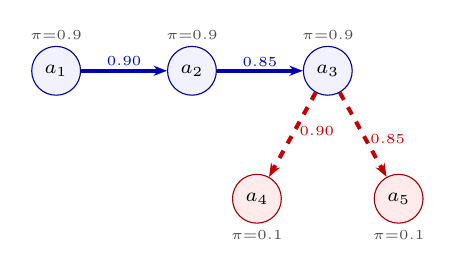
\begin{tikzpicture}[x=15mm, y=13mm]
  % --- the three TRUE claims: a support chain ----------------------------
  \node[atomtrue]  (a1) at (0,0)    {$a_1$};
  \node[atomtrue]  (a2) at (1.15,0) {$a_2$};
  \node[atomtrue]  (a3) at (2.3,0)  {$a_3$};
  % --- the two FALSE claims: attributed and rejected ---------------------
  \node[atomfalse] (a4) at (1.7,-1.25) {$a_4$};
  \node[atomfalse] (a5) at (2.9,-1.25) {$a_5$};

  \node[prlab,above=0.4mm of a1] {$\pi{=}0.9$};
  \node[prlab,above=0.4mm of a2] {$\pi{=}0.9$};
  \node[prlab,above=0.4mm of a3] {$\pi{=}0.9$};
  \node[prlab,below=0.4mm of a4] {$\pi{=}0.1$};
  \node[prlab,below=0.4mm of a5] {$\pi{=}0.1$};

  \draw[ent,relw=0.90] (a1) -- (a2) node[wlab,above]{$0.90$};
  \draw[ent,relw=0.85] (a2) -- (a3) node[wlab,above]{$0.85$};
  % the rejections: a true claim contradicts each false one
  \draw[con,relw=0.90] (a3) -- (a4) node[wlab,right,pos=0.45]{$0.90$};
  \draw[con,relw=0.85] (a3) -- (a5) node[wlab,right,pos=0.55]{$0.85$};
\end{tikzpicture}}
\caption{\textbf{Response A, coherent.} The three true claims form a support chain
  ($a_1\!\to\!a_2\!\to\!a_3$) and each false claim is \emph{attributed and rejected}
  by a \con{} edge from $a_3$. Every claim ends on the correct side of its own prior:
  $\LCS_{\mm}=0.590$, $\LCS_{\cons}=0.963$, $\log Z=-0.95$.}
\label{fig:pair-coherent}
\end{subfigure}
\hfill
\begin{subfigure}[t]{0.49\textwidth}
\centering
\resizebox{\linewidth}{!}{%
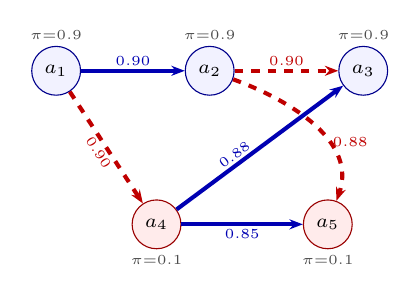
\begin{tikzpicture}[x=15mm, y=13mm]
  \node[atomtrue]  (a1) at (0,0)       {$a_1$};
  \node[atomtrue]  (a2) at (1.3,0)     {$a_2$};
  \node[atomtrue]  (a3) at (2.6,0)     {$a_3$};
  \node[atomfalse] (a4) at (0.85,-1.5) {$a_4$};
  \node[atomfalse] (a5) at (2.3,-1.5)  {$a_5$};

  \node[prlab,above=0.4mm of a1] {$\pi{=}0.9$};
  \node[prlab,above=0.4mm of a2] {$\pi{=}0.9$};
  \node[prlab,above=0.4mm of a3] {$\pi{=}0.9$};
  \node[prlab,below=0.4mm of a4] {$\pi{=}0.1$};
  \node[prlab,below=0.4mm of a5] {$\pi{=}0.1$};

  \draw[ent,relw=0.90] (a1) -- (a2) node[wlab,above]{$0.90$};
  % the response contradicts its own chain ...
  \draw[con,relw=0.90] (a2) -- (a3) node[wlab,above]{$0.90$};
  % ... and leans on a FALSE claim as a load-bearing premise for a TRUE one
  \draw[ent,relw=0.88] (a4) -- (a3) node[wlab,above,sloped,pos=0.38]{$0.88$};
  \draw[con,relw=0.90] (a1) -- (a4) node[wlab,below,sloped]{$0.90$};
  \draw[ent,relw=0.85] (a4) -- (a5) node[wlab,below]{$0.85$};
  \draw[con,relw=0.88] (a2) to[out=-20,in=70] node[wlab,right,pos=0.62]{$0.88$} (a5);
\end{tikzpicture}}
\caption{\textbf{Response B, incoherent.} The same five claims. The response
  contradicts its own chain ($a_2\!\not\to\!a_3$) and makes the false $a_4$ a
  load-bearing premise for the true $a_3$, while $a_1$ and $a_2$ deny $a_4$ and
  $a_5$. The \emph{true} claim $a_3$ is dragged to $0.513$ --- far below its own
  $0.9$ prior: $\LCS_{\mm}=0.494$, $\LCS_{\cons}=0.414$, $\log Z=-3.78$.}
\label{fig:pair-incoherent}
\end{subfigure}
\caption{Relation graphs for the five-claim worked pair (\S\ref{sec-examples}).
  Blue nodes are claims true of the world ($\pi_i=0.9$), red nodes false
  ($\pi_i=0.1$); the \emph{same} five claims appear in both panels. Solid blue:
  \ent{}; dashed red: \con{}. Line width grows with the relation weight $p$.
  The panels differ only in \emph{how the response arranges} the claims, which is
  the whole of what coherence measures --- no per-claim factuality check can
  separate them.}
\label{fig:pair-graphs}
\end{figure}

% The coherence MRF of the five-claim worked pair, drawn as an explicit bipartite
% factor graph: circles are the binary claim variables, squares the factors of
% Eq. eq-joint -- grey unaries phi_i (the priors) and black pairwise psi_r (the
% relations). Styles are in preamble.tex.
\begin{figure}[t]
\centering
\begin{subfigure}[t]{0.49\textwidth}
\centering
\resizebox{\linewidth}{!}{%
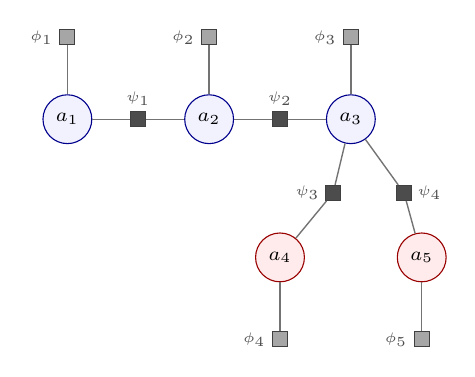
\begin{tikzpicture}[x=15mm, y=13mm]
  \node[atomtrue]  (a1) at (0,0)       {$a_1$};
  \node[atomtrue]  (a2) at (1.2,0)     {$a_2$};
  \node[atomtrue]  (a3) at (2.4,0)     {$a_3$};
  \node[atomfalse] (a4) at (1.8,-1.35) {$a_4$};
  \node[atomfalse] (a5) at (3.0,-1.35) {$a_5$};

  % unary factors phi_i = [1-pi_i, pi_i]
  \node[unary] (p1) at (0,0.8)       {}; \draw[flink] (p1) -- (a1);
  \node[unary] (p2) at (1.2,0.8)     {}; \draw[flink] (p2) -- (a2);
  \node[unary] (p3) at (2.4,0.8)     {}; \draw[flink] (p3) -- (a3);
  \node[unary] (p4) at (1.8,-2.15)   {}; \draw[flink] (p4) -- (a4);
  \node[unary] (p5) at (3.0,-2.15)   {}; \draw[flink] (p5) -- (a5);
  \node[prlab,left=0.4mm of p1] {$\phi_1$};
  \node[prlab,left=0.4mm of p2] {$\phi_2$};
  \node[prlab,left=0.4mm of p3] {$\phi_3$};
  \node[prlab,left=0.4mm of p4] {$\phi_4$};
  \node[prlab,left=0.4mm of p5] {$\phi_5$};

  % pairwise factors psi_r, one per relation
  \node[factor] (f12) at (0.6,0)   {}; \draw[flink] (a1) -- (f12) -- (a2);
  \node[factor] (f23) at (1.8,0)   {}; \draw[flink] (a2) -- (f23) -- (a3);
  \node[factor] (f34) at (2.25,-0.72) {}; \draw[flink] (a3) -- (f34) -- (a4);
  \node[factor] (f35) at (2.85,-0.72) {}; \draw[flink] (a3) -- (f35) -- (a5);
  \node[prlab,above=0.3mm of f12] {$\psi_1$};
  \node[prlab,above=0.3mm of f23] {$\psi_2$};
  \node[prlab,left=0.3mm of f34]  {$\psi_3$};
  \node[prlab,right=0.3mm of f35] {$\psi_4$};
\end{tikzpicture}}
\caption{\textbf{Response A.} Five unaries and four pairwise factors.}
\label{fig:mrf-coherent}
\end{subfigure}
\hfill
\begin{subfigure}[t]{0.49\textwidth}
\centering
\resizebox{\linewidth}{!}{%
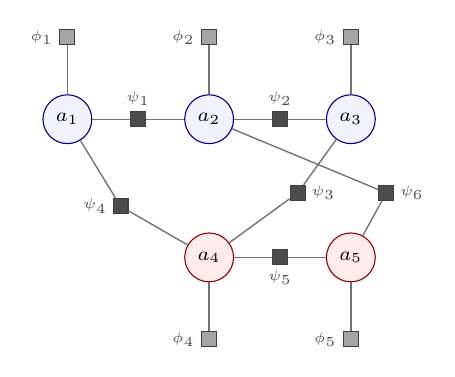
\begin{tikzpicture}[x=15mm, y=13mm]
  \node[atomtrue]  (a1) at (0,0)       {$a_1$};
  \node[atomtrue]  (a2) at (1.2,0)     {$a_2$};
  \node[atomtrue]  (a3) at (2.4,0)     {$a_3$};
  \node[atomfalse] (a4) at (1.2,-1.35) {$a_4$};
  \node[atomfalse] (a5) at (2.4,-1.35) {$a_5$};

  \node[unary] (p1) at (0,0.8)     {}; \draw[flink] (p1) -- (a1);
  \node[unary] (p2) at (1.2,0.8)   {}; \draw[flink] (p2) -- (a2);
  \node[unary] (p3) at (2.4,0.8)   {}; \draw[flink] (p3) -- (a3);
  \node[unary] (p4) at (1.2,-2.15) {}; \draw[flink] (p4) -- (a4);
  \node[unary] (p5) at (2.4,-2.15) {}; \draw[flink] (p5) -- (a5);
  \node[prlab,left=0.4mm of p1] {$\phi_1$};
  \node[prlab,left=0.4mm of p2] {$\phi_2$};
  \node[prlab,left=0.4mm of p3] {$\phi_3$};
  \node[prlab,left=0.4mm of p4] {$\phi_4$};
  \node[prlab,left=0.4mm of p5] {$\phi_5$};

  \node[factor] (f12) at (0.6,0)      {}; \draw[flink] (a1) -- (f12) -- (a2);
  \node[factor] (f23) at (1.8,0)      {}; \draw[flink] (a2) -- (f23) -- (a3);
  \node[factor] (f43) at (1.95,-0.72) {}; \draw[flink] (a4) -- (f43) -- (a3);
  \node[factor] (f14) at (0.45,-0.85) {}; \draw[flink] (a1) -- (f14) -- (a4);
  \node[factor] (f45) at (1.8,-1.35)  {}; \draw[flink] (a4) -- (f45) -- (a5);
  \node[factor] (f25) at (2.7,-0.72)  {}; \draw[flink] (a2) -- (f25) -- (a5);
  \node[prlab,above=0.3mm of f12] {$\psi_1$};
  \node[prlab,above=0.3mm of f23] {$\psi_2$};
  \node[prlab,right=0.3mm of f43] {$\psi_3$};
  \node[prlab,left=0.3mm of f14]  {$\psi_4$};
  \node[prlab,below=0.3mm of f45] {$\psi_5$};
  \node[prlab,right=0.3mm of f25] {$\psi_6$};
\end{tikzpicture}}
\caption{\textbf{Response B.} The same five unaries, but six pairwise factors
  wired so that $\psi_3$ makes a false claim a premise for a true one.}
\label{fig:mrf-incoherent}
\end{subfigure}
\caption{The coherence MRF of Eq.~\ref{eq-joint} for the two responses, as an
  explicit factor graph. Circles are the binary claim variables; grey squares the
  unary factors $\phi_i=[1-\pi_i,\,\pi_i]$ that carry the priors; black squares
  the pairwise factors $\psi_{\tau_r,p_r}$ of Table~\ref{tab:factors}, one per
  mined relation. \textbf{The priors enter only through the $\phi_i$}: the
  claim-level potentials are identical across the two panels, and every difference
  in score comes from the $\psi_r$ --- their number, their endpoints, and their
  couplings.}
\label{fig:pair-mrfs}
\end{figure}


The point of this example is that factuality and coherence are separable, so we hold the first
fixed and vary only the second. Five claims about the Voyager~1 mission are fixed once and for all,
three of them true of the world and two false; stage one is taken as given, contributing the priors
$\pi=0.9$ for each true claim and $\pi=0.1$ for each false one through the composition of \S\ref{sec-twostage}:

\begin{center}\small
\begin{tabularx}{0.93\textwidth}{@{}l l c X@{}}
\toprule
 & & $\pi_i$ & Claim \\
\midrule
$a_1$ & true  & $0.9$ & Voyager~1 crossed the heliopause in August 2012. \\
$a_2$ & true  & $0.9$ & After the crossing, Voyager~1's instruments measured a sharp rise in plasma density. \\
$a_3$ & true  & $0.9$ & Voyager~1 is therefore in interstellar space. \\
$a_4$ & false & $0.1$ & Voyager~1's plasma wave instrument failed permanently before the crossing. \\
$a_5$ & false & $0.1$ & Voyager~1 has left the Solar System entirely. \\
\bottomrule
\end{tabularx}
\end{center}

Two responses then assert \emph{these same five claims} and differ only in how they arrange them.
Because the claim set is identical, every per-claim factuality check returns the same verdict on
both; the relation graphs (Figure~\ref{fig:pair-graphs}) and the MRFs they induce
(Figure~\ref{fig:pair-mrfs}) are what differ. Table~\ref{tab:pair-responses} gives both responses in
full, with the span asserting each claim marked \claimref{i} at its first mention.

\begin{table}[tbp]
\centering\small
\begin{tabularx}{0.96\textwidth}{@{}X@{}}
\toprule
\textbf{Response A} (coherent) --- $\LCS_{\mm}=0.590$, $\LCS_{\cons}=0.963$, $\log Z=-0.95$ \\
\midrule
Voyager~1 crossed the heliopause in August 2012,\,\claimref{1} and in the days that followed its
instruments measured a sharp rise in plasma density\,\claimref{2} --- the signature of the denser
medium beyond, and \emph{the measurement that established the boundary had been passed.}
Voyager~1 is therefore in interstellar space.\,\claimref{3} Two persistent misconceptions are
worth clearing up. The first is that the probe's plasma wave instrument had failed permanently
before the crossing;\,\claimref{4} \emph{it cannot have, since it is precisely that instrument
which returned the density profile the conclusion rests on.} The second is that Voyager~1 has
left the Solar System altogether.\,\claimref{5} \emph{Being in interstellar space is not the same
thing: the Sun's gravitational reach extends through the Oort cloud, far beyond the probe's
present distance.} \\
\addlinespace[4pt]
\midrule
\textbf{Response B} (incoherent) --- $\LCS_{\mm}=0.494$, $\LCS_{\cons}=0.414$, $\log Z=-3.78$ \\
\midrule
Voyager~1 crossed the heliopause in August 2012,\,\claimref{1} and after the crossing its
instruments measured a sharp rise in plasma density.\,\claimref{2}
\emph{That said, the probe cannot really be counted as being in interstellar space.}\,\claimref{3} The plasma wave instrument
had in fact failed permanently before the crossing,\,\claimref{4} \emph{and it is precisely that
failure which tells us the probe reached interstellar space.} The instrument failure also means
Voyager~1 has left the Solar System entirely.\,\claimref{5} \emph{Of course, the August 2012
crossing rules out any such permanent failure, and the density measurement is flatly inconsistent
with the probe having left the Solar System.} \\
\bottomrule
\end{tabularx}
\caption{The two responses in full. They assert the \emph{same} five claims of
  \S\ref{sec-example-pair}; each claim's first mention is marked \claimref{i}. Italicized spans are
  the ones the estimator reads as relations. In A they discharge the two false claims; in B they
  reason \emph{from} them.}
\label{tab:pair-responses}
\end{table}

\begin{table}[tbp]
\centering\footnotesize
\setlength{\tabcolsep}{4pt}
\renewcommand{\arraystretch}{1.2}
\caption{The mined relations of both responses, one row per claim pair. \textsc{s} is the Level-2
  discourse sense, $\tau$ the Level-1 coupling it compiles to (Table~\ref{tab:compile}), $p$ the
  weight. \textsc{e} abbreviates \ent{}, \textsc{c} \con{}. These are exactly the edges of
  Figure~\ref{fig:pair-graphs} and the factors $\psi_r$ of Figure~\ref{fig:pair-mrfs}; a dash means
  the response draws no relation over that pair.}
\label{tab:pair-relations}
\begin{tabularx}{\textwidth}{@{}l@{\hspace{7pt}} ll c c@{\hspace{7pt}} ll c c@{\hspace{6pt}} X@{}}
\toprule
& \multicolumn{4}{c@{\hspace{7pt}}}{\textbf{Response A} (coherent)}
& \multicolumn{4}{c@{\hspace{6pt}}}{\textbf{Response B} (incoherent)} & \\
\cmidrule(r{5pt}){2-5}\cmidrule(r{4pt}){6-9}
Pair & Edge & \textsc{s} & $\tau$ & $p$ & Edge & \textsc{s} & $\tau$ & $p$ & What differs \\
\midrule
$\{a_1,a_2\}$ & $a_1\!\to\!a_2$ & \sense{Cau-Eff} & \textsc{e} & $.90$
              & $a_1\!\to\!a_2$ & \sense{Cau-Eff} & \textsc{e} & $.90$
  & The one relation both agree on. \\
$\{a_2,a_3\}$ & $a_2\!\to\!a_3$ & \sense{Evidence} & \textsc{e} & $.85$
              & $a_2\!\to\!a_3$ & \sense{Contrast} & \textsc{c} & $.90$
  & A supports its conclusion; B denies it. Support becomes conflict. \\
$\{a_3,a_4\}$ & $a_3\!\to\!a_4$ & \sense{Contrast} & \textsc{c} & $.90$
              & $a_4\!\to\!a_3$ & \sense{Evidence} & \textsc{e} & $.88$
  & \textbf{The arrow reverses.} A rejects $a_4$; B makes it a premise. \\
$\{a_3,a_5\}$ & $a_3\!\to\!a_5$ & \sense{Contrast} & \textsc{c} & $.85$
              & \multicolumn{4}{c@{\hspace{6pt}}}{---}
  & A refuses $a_5$; B never draws the distinction. \\
$\{a_4,a_5\}$ & \multicolumn{4}{c@{\hspace{7pt}}}{---}
              & $a_4\!\to\!a_5$ & \sense{Cau-Eff} & \textsc{e} & $.85$
  & B alone chains one falsehood into the other. \\
$\{a_1,a_4\}$ & \multicolumn{4}{c@{\hspace{7pt}}}{---}
              & $a_1\!\to\!a_4$ & \sense{Contrast} & \textsc{c} & $.90$
  & B denies $a_4$, which it had just used as a premise --- this strands $a_3$. \\
$\{a_2,a_5\}$ & \multicolumn{4}{c@{\hspace{7pt}}}{---}
              & $a_2\!\to\!a_5$ & \sense{Contrast} & \textsc{c} & $.88$
  & Likewise for $a_5$: asserted, then denied. \\
\midrule
\textbf{Totals} & \multicolumn{4}{c@{\hspace{7pt}}}{2 \textsc{e}, 2 \textsc{c}}
                & \multicolumn{4}{c@{\hspace{6pt}}}{3 \textsc{e}, 3 \textsc{c}}
  & A's conflicts point \emph{outward}, at the false claims; half of B's point \emph{inward}. \\
\bottomrule
\end{tabularx}
\end{table}

The italicized spans are the ones the estimator reads as relations, and they are the whole
difference between the two. Table~\ref{tab:pair-relations} lays the two relation sets side by side,
one row per claim pair, with each relation's discourse sense and the coupling it compiles to. In A
the false claims are named, attributed, and then refused on a stated ground, which compiles to a
\con{} edge from $a_3$. In B the same falsehoods are named and then \emph{used} --- $a_4$ is offered
as the reason $a_3$ holds --- while the response also denies $a_3$ outright and, in its last
sentence, denies $a_4$ and $a_5$ too. Mentioning a falsehood is not what costs B its score;
asserting it and reasoning from it is. All values below are exact, by $2^5=32$-world enumeration.

\begin{example}[Coherent]
\label{ex-pair-coherent}
Response~A's four relations (Table~\ref{tab:pair-relations}, column~A) are a two-edge support chain
over the true claims and one rejection of each false claim. The model returns $\LCS_{\mm}=0.590$ and
$\LCS_{\cons}=0.963$ with $\log Z=-0.95$. Every claim finishes on the correct side of its own prior:
the true claims sit at $0.939$, $0.989$ and $0.992$ --- each \emph{above} its $0.9$ prior, because
the chain supplies mutual support --- and the false ones at $0.013$ and $0.020$, pushed below $0.1$
by the rejections. Nothing in the response fights anything else, so no claim is penalized.
\end{example}

\begin{example}[Incoherent]
\label{ex-pair-incoherent}
Response~B keeps only $a_1\!\to\!a_2$ and replaces the rest with six relations that pull against each
other (Table~\ref{tab:pair-relations}, column~B): it denies its own conclusion, promotes the false
$a_4$ to a premise for that same conclusion, chains $a_4$ into $a_5$, and then denies both
falsehoods in its closing sentence. Three of its six relations are conflicts, and two of those point
at claims the response itself asserts. The score falls to $\LCS_{\mm}=0.494$ and $\LCS_{\cons}=0.414$, with $\log Z=-3.78$. The diagnostic that
localizes the damage is per-claim: the \emph{true} $a_3$ is dragged to $0.513$, far below its own
$0.9$ prior, because its only support arrives from $a_4$, which the response itself denies --- and a
premise the text refuses cannot transmit support. Three claims finish below their own priors,
against two in Response~A, and $a_3$ is the one that matters: a claim true of the world, demoted to
a coin flip by the argument built around it.
\end{example}

Two things are worth reading off this pair. First, the priors enter \emph{only} through the unary
factors $\phi_i$ of Figure~\ref{fig:pair-mrfs}, which are identical in both panels; the entire
$0.590\to0.494$ drop is produced by the $\psi_r$, so it is attributable to arrangement alone.
Second, a claim being true of the world does not protect it: coherence is a property of the joint
distribution, and $a_3$ is suppressed by \emph{how} it is argued for, not by what it says. This is
the mechanism Remark~\ref{rem-order} anticipates and the ordering pair of
\S\ref{sec-example-order} exhibits at scale.

A caution on readouts. $\LCS_{\lp}$ is $0.194$ for Response~A and $0.267$ for Response~B, which
inverts the order --- correctly, and for a reason Eq.~\ref{eq-logz} makes plain: its references
$\log Z_{\max}$ and $\log Z_{\min}$ are recomputed \emph{per response} ($-0.49$ and $-1.06$ for A,
$-1.65$ and $-4.55$ for B), so it reports how close a response comes to the ceiling of \emph{its
own} edge skeleton, not how the two responses compare. It is a within-response diagnostic. Raw
$\log Z$ is comparable across responses and moves the right way, by $2.83$ nats.

\subsection{A sixteen-claim recall report}
\label{sec-example-aero}

% Relation graphs for the AeroParts running example.
% Edges transcribe AEROPARTS_BASE_5 / its conflict-free subset exactly
% (tests/test_lcs_relation_miner.py:83-119). Line width grows with p.
\begin{figure}[t]
\centering
\begin{subfigure}[t]{0.49\textwidth}
\centering
\resizebox{\linewidth}{!}{%
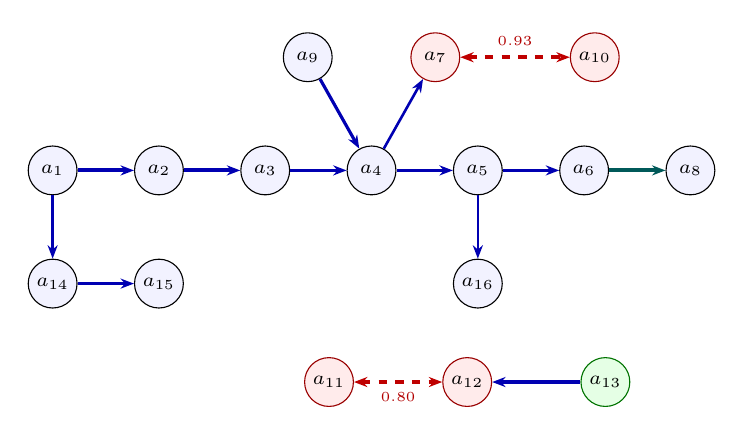
\begin{tikzpicture}[
    >={Stealth[length=1.7mm]},
    atom/.style={circle,draw,fill=blue!5,inner sep=0.5pt,minimum size=6.2mm,font=\scriptsize},
    conf/.style={circle,draw,fill=red!8,draw=red!60!black,inner sep=0.5pt,
                 minimum size=6.2mm,font=\scriptsize},
    hold/.style={circle,draw,fill=green!10,draw=green!45!black,inner sep=0.5pt,
                 minimum size=6.2mm,font=\scriptsize},
    ent/.style={-{Stealth[length=1.7mm]},blue!70!black},
    equ/.style={-{Stealth[length=1.7mm]},teal!70!black},
    xcl/.style={{Stealth[length=1.7mm]}-{Stealth[length=1.7mm]},red!75!black,dashed},
    x=13.5mm, y=12.5mm]

  % ---- the entailment spine, left to right ----
  \node[atom] (a1) at (0,0)   {$a_1$};
  \node[atom] (a2) at (1,0)   {$a_2$};
  \node[atom] (a3) at (2,0)   {$a_3$};
  \node[atom] (a4) at (3,0)   {$a_4$};
  \node[atom] (a5) at (4,0)   {$a_5$};
  \node[atom] (a6) at (5,0)   {$a_6$};
  \node[atom] (a8) at (6,0)   {$a_8$};
  % ---- branches ----
  \node[atom] (a9)  at (2.4,1.15) {$a_9$};
  \node[conf] (a7)  at (3.6,1.15) {$a_7$};
  \node[atom] (a14) at (0,-1.15)  {$a_{14}$};
  \node[atom] (a15) at (1,-1.15)  {$a_{15}$};
  \node[atom] (a16) at (4,-1.15)  {$a_{16}$};
  % ---- the blame sub-argument ----
  \node[conf] (a10) at (5.1,1.15)  {$a_{10}$};
  \node[conf] (a11) at (2.6,-2.15) {$a_{11}$};
  \node[conf] (a12) at (3.9,-2.15) {$a_{12}$};
  \node[hold] (a13) at (5.2,-2.15) {$a_{13}$};

  \draw[ent,line width=1.50pt] (a1) -- (a2);
  \draw[ent,line width=1.42pt] (a2) -- (a3);
  \draw[ent,line width=1.10pt] (a3) -- (a4);
  \draw[ent,line width=1.30pt] (a4) -- (a5);
  \draw[ent,line width=1.22pt] (a5) -- (a6);
  \draw[ent,line width=0.94pt] (a4) -- (a7);
  \draw[ent,line width=1.14pt] (a9) -- (a4);
  \draw[equ,line width=1.46pt] (a6) -- (a8);
  \draw[ent,line width=1.26pt] (a1) -- (a14);
  \draw[ent,line width=1.10pt] (a14) -- (a15);
  \draw[ent,line width=0.86pt] (a5) -- (a16);
  \draw[ent,line width=1.42pt] (a13) -- (a12);

  % ---- the two conflicts: what makes this response incoherent ----
  \draw[xcl,line width=1.58pt] (a7) -- (a10)
        node[midway,above,font=\tiny,red!70!black]{$0.93$};
  \draw[xcl,line width=1.30pt] (a11) -- (a12)
        node[midway,below,font=\tiny,red!70!black]{$0.80$};
\end{tikzpicture}}
\caption{\textbf{Incoherent} (base). Two \coupling{exclusive} conflicts (dashed):
  $a_7\!\leftrightarrow\!a_{10}$ is \emph{unresolved}; $a_{11}\!\leftrightarrow\!a_{12}$
  is a concession the holding $a_{13}$ (green) resolves.
  $\readout{mm}=0.607$, $\log Z=-9.64$.}
\label{fig:aero-incoherent}
\end{subfigure}
\hfill
\begin{subfigure}[t]{0.49\textwidth}
\centering
\resizebox{\linewidth}{!}{%
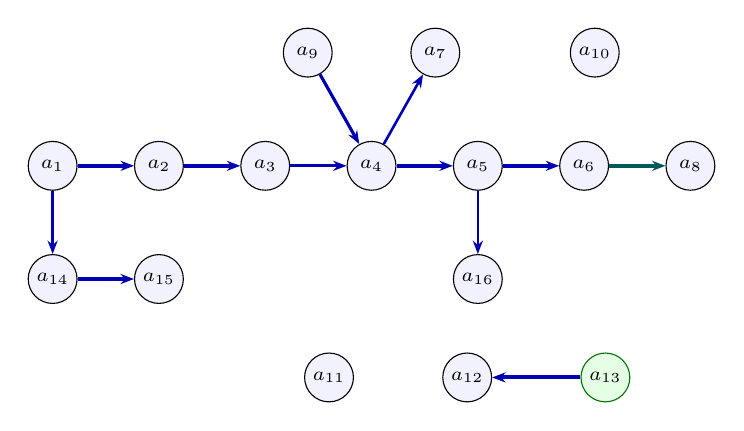
\begin{tikzpicture}[
    >={Stealth[length=1.7mm]},
    atom/.style={circle,draw,fill=blue!5,inner sep=0.5pt,minimum size=6.2mm,font=\scriptsize},
    hold/.style={circle,draw,fill=green!10,draw=green!45!black,inner sep=0.5pt,
                 minimum size=6.2mm,font=\scriptsize},
    ent/.style={-{Stealth[length=1.7mm]},blue!70!black},
    equ/.style={-{Stealth[length=1.7mm]},teal!70!black},
    x=13.5mm, y=12.5mm]

  \node[atom] (a1) at (0,0)   {$a_1$};
  \node[atom] (a2) at (1,0)   {$a_2$};
  \node[atom] (a3) at (2,0)   {$a_3$};
  \node[atom] (a4) at (3,0)   {$a_4$};
  \node[atom] (a5) at (4,0)   {$a_5$};
  \node[atom] (a6) at (5,0)   {$a_6$};
  \node[atom] (a8) at (6,0)   {$a_8$};
  \node[atom] (a9)  at (2.4,1.15) {$a_9$};
  \node[atom] (a7)  at (3.6,1.15) {$a_7$};
  \node[atom] (a14) at (0,-1.15)  {$a_{14}$};
  \node[atom] (a15) at (1,-1.15)  {$a_{15}$};
  \node[atom] (a16) at (4,-1.15)  {$a_{16}$};
  \node[atom] (a10) at (5.1,1.15)  {$a_{10}$};
  \node[atom] (a11) at (2.6,-2.15) {$a_{11}$};
  \node[atom] (a12) at (3.9,-2.15) {$a_{12}$};
  \node[hold] (a13) at (5.2,-2.15) {$a_{13}$};

  \draw[ent,line width=1.50pt] (a1) -- (a2);
  \draw[ent,line width=1.42pt] (a2) -- (a3);
  \draw[ent,line width=1.10pt] (a3) -- (a4);
  \draw[ent,line width=1.30pt] (a4) -- (a5);
  \draw[ent,line width=1.22pt] (a5) -- (a6);
  \draw[ent,line width=0.94pt] (a4) -- (a7);
  \draw[ent,line width=1.14pt] (a9) -- (a4);
  \draw[equ,line width=1.46pt] (a6) -- (a8);
  \draw[ent,line width=1.26pt] (a1) -- (a14);
  \draw[ent,line width=1.10pt] (a14) -- (a15);
  \draw[ent,line width=0.86pt] (a5) -- (a16);
  \draw[ent,line width=1.42pt] (a13) -- (a12);
\end{tikzpicture}}
\caption{\textbf{Coherent}. The identical support structure with both conflict edges
  removed; $a_{10}$ and $a_7$ are no longer suppressed.
  $\readout{mm}=0.620$, $\log Z=-8.25$, $\readout{lp}=1.00$.}
\label{fig:aero-coherent}
\end{subfigure}
\caption{Relation graphs for the AeroParts recall report
  (\S\ref{sec-examples}). Solid blue: \coupling{entailment}; teal:
  \coupling{equivalence}; dashed red, double-headed: \coupling{exclusive}. Line
  width grows with the relation weight $p$. \textbf{The two panels differ only in
  the two conflict edges}, so the $0.607\!\to\!0.620$ lift and the $1.39$ nats of
  recovered mass are attributable to conflict structure alone.}
\label{fig:aero-graphs}
\end{figure}


The second example is a sixteen-claim aviation recall report, which exercises the conflict taxonomy
more fully than the five-claim pair: it carries both an unresolved conflict and a conceded one. Its
relation graph is twelve support edges ---
an entailment spine $a_1\!\to\!a_2\!\to\!\dots\!\to\!a_6$ (shipment certified to spec, installation,
entry into service, in-flight failures, regulatory probe, grounding order), branches to the
pulled-from-service claim, the maintenance-log evidence, the tribunal's damages award and the
regulator's bulletin, and one \eqv{} edge --- plus two conflicts. Every value below is exact, by
$2^{16}$ enumeration, and the graph is reproduced edge-by-edge in Figure~\ref{fig:aero-graphs} with
each edge's weight shown by line thickness.

\begin{example}[Incoherent]
\label{ex-incoherent}
The report asserts both that \emph{no passengers or crew were harmed} and that a wire report
\emph{claimed three passengers died}. These are exhaustive alternatives rather than mere opposition:
they cannot both hold and cannot both fail, so the relation is \exc{} with $p=0.93$ --- and nothing in
the response resolves it. A second tension, between the airline's pilot-error argument and the final
report's metallurgical-defect finding ($p=0.80$), is a \sense{Concession} that the tribunal's holding
does resolve, and Eq.~\ref{eq-concession} discounts it accordingly. The model returns
$\LCS_{\mm}=0.607$ with $\log Z=-9.64$. The diagnostic that localizes the incoherence is per-claim: the
marginal of the claim on the losing side of the \emph{unresolved} conflict is dragged \emph{below its
own prior}, which no aggregate score would reveal. Applying the concession discount alone --- resolving
the second tension while leaving the first --- raises the score to $0.612$, as C2 requires.
\end{example}

\begin{example}[Coherent]
\label{ex-coherent}
Removing the two conflict edges and changing nothing else leaves the identical support structure
(Figure~\ref{fig:aero-coherent}). The score rises to $\LCS_{\mm}=0.620$ with $\log Z=-8.25$ and
$\LCS_{\lp}=1.00$: the response is now as coherent as its own edge skeleton permits, which is what the
ceiling of Eq.~\ref{eq-logz} means. The suppressed claim recovers to its prior.
\end{example}

Because the two panels of Figure~\ref{fig:aero-graphs} differ \emph{only} in the two conflict edges,
the $0.607\to0.620$ lift and the $1.39$ nats of recovered probability mass are attributable to conflict
structure alone --- which is the property the ladder construction of \S\ref{sec-protocol} generalizes
from one pair to a family. The full ladder over this family is monotone throughout:
$0.586 < 0.607 < 0.612 < 0.613 < 0.620$ over the rungs \emph{worse}, \emph{base},
\emph{concession-resolved}, \emph{one-conflict-fixed}, \emph{coherent}.\footnote{Treating both tensions
as plain \con{} rather than \exc{} --- the three-coupling model that omits the exhaustiveness
distinction --- gives $\LCS_{\mm}=0.587$ and $\log Z=-9.75$ for Example~\ref{ex-incoherent}, with
Example~\ref{ex-coherent} unchanged at $0.620$ and $-8.25$. The distinction of \S\ref{sec-levels} is
worth $0.020$ of score here, and the reason it matters more than that figure suggests is
Table~\ref{tab:allcands}: with \exc{} conflicts, readout (b)'s conflict term is pinned at $1.000$ and
the readout fails outright.}

\subsection{A claim-identical ordering pair}
\label{sec-example-order}

This pair makes the order-sensitivity claim concretely. Two summaries of one appellate
judgment are built from an \emph{identical} set of eighteen claims --- the same atom texts, one a
permutation of the other --- differing only in whether self-serving assertions precede or follow the
findings that qualify them. The faithful ordering scores $\LCS_{\mm}=0.95$ and the
self-serving-first ordering $0.90$. No per-claim factuality check can separate them, because every
claim is byte-identical; what differs is which claims the response leaves standing unqualified at the
point where it asserts them.

It is worth being exact about \emph{how} the two scores differ, because Remark~\ref{rem-order} might
seem to forbid it: nothing in Eq.~\ref{eq-joint} references position, so an edit preserving the
relation set cannot move any readout. The pair does not preserve the relation set. Mining is
response-grounded (\S\ref{sec-mining}), so the relations the estimator draws are a function of the
prose, not of the claim list: the faithful summary states each tension beside the truth or holding
that settles it, which the estimator reads as a \sense{Concession} the text resolves and
Eq.~\ref{eq-concession} discounts; the adversarial summary leaves the same claims standing
unqualified until a later holding overrides them, which reads as a live conflict. The claim set is
what factuality sees and it is identical; the relation set is what coherence sees and it is not.


%% ================================================================
\section{\texorpdfstring{$k$}{k}-ary representability}
\label{app-kary}
%% ================================================================

This appendix proves Prop.~\ref{prop-kary} of \S\ref{sec-limitations} and quantifies the gap it
describes.

\begin{proof}[Proof of Prop.~\ref{prop-kary}]
By Eq.~\ref{eq-joint}, $\pr{1,1,1}=Z^{-1}\prod_i\phi_i(1)\prod_{i<j}\psi_{ij}(1,1)$, a product of
non-negative terms, which vanishes only if some term does. If $\phi_i(1)=0$ then $a_i$ is false almost
surely and both pairs containing $i$ have probability zero. If $\psi_{ij}(1,1)=0$ then every world with
$a_i=a_j=1$ carries that factor, so $\pr{a_i{=}1,a_j{=}1}=0$ directly. A ternary factor that vanishes
only at $(1,1,1)$ has neither consequence.
\end{proof}

The gap is quantitative as well as qualitative. With uniform priors, a ternary factor supported off
$(1,1,1)$ gives $\pr{1,1,1}=0$ while leaving each pair jointly true with probability $0.143$; the best
pairwise attempt that drives $\pr{1,1,1}$ below $10^{-4}$ leaves the pairs at $0.028$, and a random
search over $2\times10^{5}$ pairwise parameterizations found nothing better. The pairwise model can only
suppress the bad world by also suppressing the good ones that share a $(1,1)$ cell with it. Every figure
here is exact by $2^3$ enumeration and reproduced by a released script and regression test, so the
proposition is checked and not merely asserted.

On the three-claim arithmetic instance of \S\ref{sec-limitations} --- a league of $356$ teams forming
$32$ conferences of exactly $10$ members --- the readouts report the passage as coherent at
$\LCS_{\mm}=0.68$ and $\LCS_{\lp}=1.00$. Prop.~\ref{prop-kary} says no reweighting of the pairwise
factors could have helped. Of the two milder consequences named in \S\ref{sec-limitations},
transitivity is the more visible: the model will happily hold $a\Rightarrow b$ and $b\Rightarrow c$ at
high weight while leaving $a$ and $c$ unrelated, since it has no rule tying them.


%% ================================================================
\section{Correspondence with Markov logic}
\label{app-mln}
%% ================================================================

The coherence MRF has a natural first-order encoding \citep{mln}, with
$\pr{\mathbf{a}}=\tfrac1Z\exp\bigl(\sum_k w_k n_k(\mathbf{a})\bigr)$ for $n_k(\mathbf{a})$ the number of
true groundings of formula $F_k$. Evidence predicates $\mathit{Entail}(i,j)$,
$\mathit{Contradict}(i,j)$, $\mathit{Equiv}(i,j)$ and $\mathit{Resolves}(h,i,j)$ carry the mined graph;
$\mathit{Holds}(i)$ is the query predicate. Working out the correspondence is instructive in both
directions.

\subsection{The naive encoding is a different model}

The obvious encoding gives each relation one weighted clause, e.g.\
$\mathit{Entail}(i,j)\wedge a_i \Rightarrow a_j$ with $w=\mathrm{logit}(p)$. This is \emph{not}
equivalent to Definition~\ref{def-mrf}. Its induced pairwise factor is $[e^w,e^w,1,e^w]$, which is not
row-stochastic in the sense of Prop.~\ref{prop-rowstoch}: it rewards the vacuous $a_s=0$ rows with
$e^w$ on \emph{both} target states, so a clause is best satisfied by making its antecedent false.
Brute force over the $2^{16}$ worlds of the recall report of \S\ref{sec-example-aero} gives mean
marginal support $0.455$ under
the naive MLN against $0.587$ under the corresponding MRF, with per-claim marginals differing by up to
$0.31$. These are two different models, not two encodings of one.

The failure is sharpest at the mode. The all-false world satisfies every implication vacuously, so under
the naive encoding the most probable configuration of any purely-implicational graph is the one in which
the response asserts nothing --- the maximum-a-posteriori reading of a response is that none of it
holds. This is Prop.~\ref{prop-vacuous} appearing in a second guise, and it is the same lesson: an
encoding that scores rule satisfaction rather than belief can be maximized by having nothing to satisfy.

\subsection{A three-clause expansion is exactly equivalent}

Writing the log-potential in the general pairwise form
$\ln\psi(a_s,a_t)=\alpha+\beta a_s+\gamma a_t+\delta\,a_s a_t$ and matching it against the
with-priors tables of Table~\ref{tab:factors} gives, for $\pi_s$ the source prior and
$\mathrm{L}(x)=\mathrm{logit}(x)$:
\begin{center}\small
\begin{tabular}{@{}lllll@{}}
\toprule
$\tau$ & $\alpha$ (unit) & $\beta$ (source) & $\gamma$ (target) & $\delta$ (conjunction) \\
\midrule
\ent & $\ln(1-\pi_s)$ & $\ln\frac{1-p}{1-\pi_s}$ & $\mathrm{L}(\pi_s)$
     & $+\mathrm{L}(p)-\mathrm{L}(\pi_s)$ \\
\con & $\ln(1-\pi_s)$ & $\ln\frac{p}{1-\pi_s}$   & $\mathrm{L}(\pi_s)$
     & $-\mathrm{L}(p)-\mathrm{L}(\pi_s)$ \\
\eqv & $\ln p$ & $\ln\frac{1-p}{p}$ & $\ln\frac{1-p}{p}$ & $+2\,\mathrm{L}(p)$ \\
\bottomrule
\end{tabular}
\end{center}
At the atom prior $\pi_s=\tfrac12$ the $\mathrm{L}(\pi_s)$ terms vanish and the table reduces to
$\gamma=0$ with $\delta=\pm\mathrm{L}(p)$: there the conjunction weight \emph{is} exactly
$\pm\mathrm{logit}(p)$, the interaction the implication was meant to carry all along, and the unit and
source clauses are the correction that makes each row a conditional. Away from $\tfrac12$ the
$\mathrm{L}(\pi_s)$ terms are load-bearing, which matters for the two-stage composition of
\S\ref{sec-twostage}, whose priors are factuality posteriors rather than uniform. With this expansion
the ground Markov logic network reproduces the MRF exactly: at $\pi_s=\tfrac12$, mean support $0.5866$
and $\log Z=-9.751$ for both, with zero per-claim difference to machine precision; the agreement is
verified against the brute-force oracle at priors on and off $\tfrac12$.

We establish the equivalence for the three original couplings only. \exc{} and \cnc{} are not tabulated
here, so the claim ``the MLN encoding reproduces the MRF'' should be read as scoped to the
three-coupling fragment. That is a real limitation for the recall report of
\S\ref{sec-example-aero}, whose conflicts are \exc{}; the five-claim pair of
\S\ref{sec-example-pair} uses \con{} throughout and so falls inside the tabulated fragment.

\subsection{Which view to keep, and why both}

The reason to prefer the MRF for the measure itself is Remark~\ref{rem-closed}: its pairwise factor
family is closed at three parameters, so the inferential vocabulary cannot quietly grow as senses are
added, and every relation type is guaranteed to be a $2\times2$ potential. The reason to keep the
Markov logic view is that the rules our model cannot express are naturally written there --- a
transitivity rule $\mathit{Entail}(i,j)\wedge\mathit{Entail}(j,k)\Rightarrow\mathit{Entail}(i,k)$, a
concession-cancellation rule $\mathit{Resolves}(h,i,j)\wedge a_h \Rightarrow \neg\mathit{Penalize}(i,j)$
replacing the fixed discount of Eq.~\ref{eq-concession}, and a double-conflict rule --- and their
weights could be \emph{learned} from labelled ladders rather than set by hand. That is the route past
the two limitations \S\ref{sec-limitations} names, and it requires an MLN solver (MC-SAT for marginals,
MaxWalkSAT for the mode) rather than the bucket-elimination stack used here.


%% ================================================================
\section{The reified coherence node, worked}
\label{app-reified}
%% ================================================================

To make Eq.~\ref{eq-reified} concrete, take the three-claim subnet consisting of the unresolved
casualty conflict of Example~\ref{ex-incoherent} together with one entailment feeding it: claims
$a_7,a_{10}$ joined by a conflict at $p=0.93$, and $a_4\to a_7$ an entailment at $p=0.65$, all priors
$\tfrac12$, with $\rho=\tfrac12$. Writing out the eight-cell vote factor for each relation from
Eq.~\ref{eq-reified} and enumerating the $2^4$ worlds of $(a_4,a_7,a_{10},R)$ gives
$\pr{R{=}1}=0.453$: below its prior, because both relations have violating worlds that carry
appreciable mass, and the conflict's violating world $(1,1)$ carries the most.

Two properties of the construction are worth noting. The $R=0$ branch is flat, so $R=0$ asserts nothing
and the node cannot be driven up merely by adding relations that happen to be satisfied. And the factor
is a \emph{noisy} AND rather than a hard one: a relation with $p_r<1$ leaves some mass on its violating
worlds even when $R=1$, so a single strongly-violated relation reduces $\pr{R{=}1}$ without pinning it
to zero. The reason we do not adopt the readout despite this reasonable behaviour is
Table~\ref{tab:allcands}: it dips at the concession variant for the reason of
Prop.~\ref{prop-quirk}, and it requires the free parameter $\rho$, violating R4.


%% ================================================================
\section{The estimation prompts, verbatim}
\label{app-prompts}
%% ================================================================

The four prompts below are reproduced exactly as they are issued, extracted programmatically from the
released source so that this appendix cannot drift from the code. Placeholders in double braces are
substituted at call time; \verb|{{sense_menu}}| is substituted at build time from one of the two menus
in \S\ref{app-menus}.

\subsection{Prompt A, first generation --- discourse sense and coupling}
\label{app-prompt-a1}
$6{,}148$ characters. Placeholders: \verb|{{sense_menu}}|, \verb|{{response}}|, \verb|{{atom_a}}|,
\verb|{{atom_b}}|.
\promptfile{prompts/PROMPT_A_V1.txt}

\subsection{Prompt A, second generation --- rebalanced for precision}
\label{app-prompt-a2}
$6{,}361$ characters. Same placeholders. The five changes relative to the first generation, and their
motivation, are given in \S\ref{sec-mining}: few-shot balance from $3{:}1$ related to $2{:}3$; negative
exemplars showing silence rather than explicit disavowal; a verifiable evidence span; the
discriminating question asked first; and \coupling{none} given first position and equal prose.
Transitivity is named as a non-relation.
\promptfile{prompts/PROMPT_A_V2.txt}

\subsection{Prompt B, default --- surrogate-token conditional strength}
\label{app-prompt-b1}
$2{,}182$ characters. Placeholders: \verb|{{response}}|, \verb|{{atom_a}}|, \verb|{{atom_b}}|,
\verb|{{coupling}}| (twice). This is the one prompt that does not end in a newline: it terminates with
\verb|Answer: | including the trailing space, so that the model's next token is the surrogate whose
logprobs are read. Reproducing it without that trailing space changes the tokenization of the answer
position and therefore the estimate.
\promptfile{prompts/PROMPT_B_SURROGATE.txt}

\subsection{Prompt B, baseline --- verbalized conditional strength}
\label{app-prompt-b2}
$2{,}112$ characters. Retained only for the comparison reported in \S\ref{sec-experiments}; verbalized
confidence is weakly calibrated \citep{xiong}.
\promptfile{prompts/PROMPT_B_VERBALIZED.txt}

\subsection{The two sense menus}
\label{app-menus}
The full menu offers all twelve senses of Table~\ref{tab:compile} plus \coupling{none}:
\promptfile{prompts/SENSE_MENU_FULL.txt}
The restricted menu offers only the senses the evaluation corpus labels, which is the admissibility
filter of \S\ref{sec-mining} applied at elicitation time rather than after it:
\promptfile{prompts/SENSE_MENU_GOLD9.txt}
Note that the restricted menu omits \sense{Succession} as well as \sense{Condition} and
\sense{Instantiation}, leaving nine relation-bearing senses. \sense{Succession} is dropped because it is
the mirror of \sense{Precedence} and both compile to \coupling{none}, so offering both invites an
arbitrary choice on a relation that produces no factor either way. The second-generation Prompt A's body
is written against this restricted menu; when it is run with the full menu, three senses are offered
with no gloss and no coupling mapping in the prompt body, and we report which menu each source used.


%% ================================================================
\section{Serialization and the variable-ordering trap}
\label{app-uai}
%% ================================================================

One implementation detail is worth recording because it is silent when wrong. Networks are serialized in
UAI format, whose variables are identified by integer index; the index order is the sort order of
$(\text{cardinality},\text{name})$, and with uniformly binary claim variables that reduces to
\emph{lexicographic order by name}. So $a_{10}$ sorts before $a_2$. Inference returns marginals by
index, and mapping them back by any other convention --- source order, numeric order --- silently
permutes marginals across claims. The score is unchanged, since Eq.~\ref{eq-mm} is a mean, but every
per-claim diagnostic is then attributed to the wrong claim, and the ``claim dragged below its prior''
readout points at an innocent claim. The auxiliary variables of \S\ref{sec-consistency} are named with a
prefix that sorts after all claim names for the same reason, so that adding them cannot shift the claim
indices.


\end{document}
